%! Author = Marjan
%! Date = 02/02/2025
% Preamble
\documentclass[a4paper, 11pt]{book}

% Packages
\usepackage{amsmath}    % For math symbols and equations
\usepackage{graphicx}   % For including graphics
\usepackage{geometry}   % For adjusting page layout
\usepackage{fancyhdr}   % For custom headers/footers
\usepackage{hyperref}   % For hyperlinks
\usepackage{listings}   % For code listing
\usepackage{lipsum}     % For placeholder text (to test layout)
\usepackage{helvet}
\usepackage{arydshln}
\usepackage{wasysym}
\usepackage{amstex}
\usepackage{tikz} % Helvetica as a sans-serif font alternative
\renewcommand{\rmdefault}{phv} % Set the default font family to Helvetica

% Set page margins (A4 paper)
\geometry{top=1in, bottom=1in, left=1in, right=1in}

% Set up the header
\pagestyle{fancy}
\fancyhf{}
\fancyhead[L]{System Design Notes}
\fancyhead[C]{Your Name}
\fancyhead[R]{\thepage}

% Document
\begin{document}

% Title Page
    \begin{titlepage}
        \centering
        \vspace*{2in}
        \Huge \textbf{System Design Notes}
        \vfill
        \Large Your Name
        \vfill
        \Large Date: \today
    \end{titlepage}

    \newpage

    \tableofcontents
    \newpage

    \chapter{Microservices Managing the Data integrity}
Using messaging there is potential loss of the message if the MQ or the messaging broker is unavailable.
The write side, writes the data to its database but is unable to put the message on the queue.
Now the read side will never receive the message.

As a result the data across the two database instances is now in an inconsistent state.
This kind of data loss may be prevented by using a reliable messaging pattern.
In this pattern, the message is guaranteed to be delivered.
The idea is that when the right side encounters a failure on the message sent, it continues to retry until it is successful in sending the message.

These retries may cause a delay in getting to a consistent state of data across the databases instances, but the data will eventually be consistent across the database instances.

Another scenario that my lead to inconsistent state.
In this scenario the right side sends duplicate messages and the read side processes the same message, more than once and that may lead to inconsistent state.

\section{Designing for failure}
The concept of design for failure suggests that you should always anticipate that there will be failure.
As a designer of the software, you should identify the failure points in your architecture.

Consider where are the failure points?
Database may go down or even the network may not be available to a microservice inorder to connect with the message bus etc.
Even if the network is available, the external service may not be available.
So the suggestion is that once you have identified the failure points in your architecture, proactively address the failure poitns.

Note:
The best way to find out all the failure points in an architecture are to assume that there will be failures in all interfaces and components.
Database may go down.
Run out of resources, command object may not be able to push a message to the MQ due to the failure of the MQ server.
May be failures on the read side.

As a designer, once you have identified the failure points you need to think about the impact of those failure points.

Example solutions:
Write to the database and publish a message to the MQ in a single unit of work or transaction.
Two phase commit is a mechanism that can be used for carrying out the write and publish in a single unit of work or transaction.
Popular for the last three decades.
In two phase commit a distributed algorithm is used for coordinating all processes involved in the distributed transaction.
It is also referred to as the extended architecture or just ECS for short.

In the two phase commit, there is a transaction manager that coordinates the transaction across all the involved resources.

The challenge with two phase commit is that it is quite complex to implement.
A bigger issue is that a lot of distributed technologies do not support it.

Due to these challenges the two phase commit is not very popular with the designers of distributed systems.


An alternative would be to break the database writes and publish steps into two steps and use local database transactions.
In this course it is called the "reliable messaging pattern".
In this pattern, the right side writes the domain objet data and the event data in the database tables with a local transaction.
Then the evens are replayed against querying system in a separate step.

Key points.
You must identify failure points in your architecture and you must proactively address those failure points.
This is the concept of designing for failure.

Two phase commit can be used for executing distributed transaction across multiple resources.
Keeping in mind there are multiple challenges in using two phase commit for preventing the loss of messages or events.

You may use reliable messaging patterns.

%%TODO -- Address --- CQRS - Write side failures
%%TODO -- Address --- CQRS - Read side failures
%%TODO -- Handling duplicate messages

    \chapter{Introduction}


    \section{Goals of this document}
    The goal of this document is to collate information that I think is useful in the area of software architecture.


    \section{OSI Model}
    Very useful when operating on different levels of abstraction in a system

    \paragraph{Level 1} - Physical

    \paragraph{Level 2} - Data link

    \paragraph{Level 3} - Network

    \paragraph{Level 4} - Transport

    \paragraph{Level 5} - Session

    \paragraph{Level 6} - Presentation

    \paragraph{Level 7} - Application


    \section{C4 Model}
    Very useful for handling different levels of abstraction

    \paragraph{Motivations: Why should I care}
    Drivers - Performance, Scalability, Fault Tolerance.
    How to measure.....latency, throughput, cost
    Consider SLA,SLO and SLI.
    Easier to code more complex stuff......


    \chapter{Gathering requirements}
    Asking is a user is not practice.
    A better and more methodical way of gethering requires ments of the desired system is through use cases and user flows.
    A use cases are a particular scenario/ situation in whcih the system is used to achieve a userss goal.
    A user flow is a more detailed step by step graphical representation of a use case.


    \section{Gathering functional requriements}
    In a formal way.
    First we need to identify all the actors or users in out system otherwise relevant usecases may not be caught.
    Second step is to describe all the possible use cases or scenarios in which an actor can use our system.
    Finally, the third step is to take each use case and expand it through a flow of events or interactions between the actor and the system.
    In each interaction we capture the action and take a note of the data that flows with it to and from the system.

    Multiple ways to represent this, one way is a sequence diagram which is a part of UML. Standard for viaualising system design.

    \section{Non functional requirements}
    These requirements have an effect on the software architecture.

    \section{Why redesign}
    System is functionally correct but speed, scalability, maintenance or security is too hard for reasons like number of users or data volume.
    System is functionally the same after redesign.
    Right architecture from the start is important
    Quality measures are used to measure how well the system performs and correlate with the architecture.
    Quality attributes have to be measurable and testable and this must be consistent.

    Something to note is that no single architecture can provide all the quality attributes. Certain attributes contradict each other.
    Some combinations are hard/ impossible to achieve.
    Tradeoffs are needed.

    Third important consideration of the system is feasibility of the quality attributes.
    Architect needs to ensure that the system is deliverable and what the client is asking for.
    Client could actually ask for something that is not technical or not technically possible.
    I.e expensive or not feasible.
    An example could be unrealistic latency expectations.
    Before approving a requirement, consulting with a domain expert to ensure that the requirement can actually be delivered.

%    Three important quality attributes when desigining a system
    \begin{itemize}
        \item Testability and measurablility
        \item Make tradeoffs between quality attributes over others
        \item Feasibility of quality attributes
    \end{itemize}

    \section{System constraints}
    Once functional requirements are defined, system function is known there are usually multiple ways to achieve the desired system
    Quality attributes will lead to tradeoffs and this is normal.
    System constraints are referred to as pillars of an architecture.
    System constraints provide a starting point since they are usually non-negotiable and the rest of the system has to be designed around it.

    Three types

    \begin{itemize}
        \item Technical - Being locked to hardware, cloud vendors etc, must be on prem, etc.
        \item Legal - Geography, different rules in different countries where the system resides.
        \item Business - Limited budget, strict deadlines.
    \end{itemize}

    Once constraints are identified consider non-negotiable constrains and self-imposed constraints that can be removed.
    Once a set of constraints have been agreed it is hard to move away from them.
    If further in the project timeline it is found that some of those constraints were not really constraints, then the architecture will not make sense in the future.
    Another consideration is that when certain constraints are accepted, enough space needs to be left in the architecture to move away from those constraints in the future.
    Need to avoid tight coupling with certain components or constraints to allow for change otherwise whole system could be rearchitected.

    \section{Gathering System Requirements}

    \paragraph{Requirements} - Description of what we needs to be built.
    Very different when approached from a system level.
    Higher scope allows for freedom of tools and also requires a higher level of abstraction.
    Requirements are often not from an engineer or even someone technical.
    Requirements are only part of the solution.
    Client only knows the problem they need solved.
    Clarifying questions are required.

    \paragraph{Importance} - Simply build something and then fix it, wrong requirements etc, easy to fix?
    Large scale systems (i.e at this level) are big projects that cannot be changed easily.
    Many engineers involved and many hours.
    Hardware and Software costs.
    Contracts and financial obligations.
    Reputation and brand

    \section{Type of Requirements AKA Architectural Drivers}

    \paragraph{}
    Features of the System - Functional Requirements - Describe the system behaviour i.e what the system must do - Tied to the object of the system
    This doesn't determine the architecture

    \paragraph{}
    Quality Attributes - Non-functional requirements
    System properties - Scalability, Availability, Reliability, Security, Performance etc
    This does dictate the architecture

    \paragraph{}
    System Constraints - Limitations and boundaries
    Examples - Time Constraints and Deadlines, Financial Constraints, Staffing Constraints


    \chapter{Quality attributes in large scale systems}


    \section{Performance}
    Some performance metrics
    Response time - Time between client sending a request and receive a response
    Two parts, the processing time with code and databases applying business logic.
    And the waiting time.
    The duration of time that the request or response inacitvely spends in the system.
    This time is usually spend in transit in the physical network or in software queues waiting to be handled or reach its destination.
    Waiting time is also known as latency.

    Response time can also be called end to end latency and is an importnat metric.

    Another important metric is throughput, which is the amount of data a system can process in a given interval of time.
    The more per unit of time the higher the throughput.

    \subsection{Measuring}
    Consider the end to end response time.
    Consider the distribution of response times and set a measure around it.
    Use a histogram, chart etc, statistics etc.
    Especially consider tail latency, the responses that take the most time in comparison to the rest of the values.
    This tail latency needs to be as short as possible.
    Another consideration is the performance degradation point and how fast or steep the degradation is.
    This is the point in the performance graph where the performance is starting to get significantly worse as the load increases.
    Usually this means a resource is fully utilised, could be hardware resource etc or a software queue.


    \section{Scalability}
    Load and traffic patterns never stay the same.
    Seasonal, time etc.
    Scalability is a measure of a systems ability to handle a growing amount of work in an easy and cost effective way by adding resources to the system
    Optimistic scenario is linear scalability but in practice this is hard to acheieve.
    Three ways to scale
    \begin{itemize}
        \item Horizontal scaling - Add more units of the resources that we have like multiple computers.
        Spread the load.
        No limit to scala.
        Can easily add and remove systems as required.
        Provides fault tolerance and high availability straight away.
        Not every application can support this and will require code changes.
        Changes will usually be once.
        Groups of instances require more coordination and is complex.
        \item Vertical Scaling - add more CPU, higher bandwidth etc.
        Upgrade a computer.
        No code changes required.
        This has a limit and can easily reached on a global / internet system.
        Easy to do with a cloud provider.
        This can centralise the system and fail to provide fault tolerance and availability.
        \item Organisational scaling - Add more engineers.
        Before a certain point, the more engineers, the more work gets done, the more productivity is increased.
        Eventually we get less when we add too many.
        Meetings become more frequent and crowded.
        Code and merge conflicts.
        Code base will grow too large, harder for new engineers to learn the code base.
        Testing becomes hard and slow since there is no isolation, a minor change can break everything.
        Releases become risky since they include many changes.
        This impacts team scalability and engineering velocity.
    \end{itemize}
    One solution is to separate code into separate services which their own code base and tech stack, release schedule etc.

    These scalability solutions are orthogonal to each other.


    \section{Availability}
    Bad availability - Business loses money, bad things happen on important systems.
    Availability is either the fraction of time the probability that our service is operationally functional and accessible to the user.
    That time that out system is operationally functional and accessible to the user is often referred to as the uptime of the system.
    The time-out system is unavailable is referred to as downtime.
    Availability is measured as a percentage representing the ration between the uptime and the ensure time out system is running.
    This is the total sum of uptime and downtime of the system.
    Availability is measured in percentages.
    Other metrics are Mtbf and Mttr.

    Mtbf - the mean time between failures, represents the average time out system is operational.
    This is useful when dealing with multiple pieces of hardware. Most stuff is on the cloud and this avialable upfront.

    mTOR - mean time for recovery - the average time it takes to detect and recover from a failure, which is the average down time of our system.
    Until failure is recovered from the system is essentially non-operational.

    Availability of a system is the mtbf divided by the sum of mtbf and mttr.
    Use formula to estimate availability.
%    Add equation
    Note: If we minimise the average time to detect and recover from a failure theoretically all the wy to 0 we can essentially achieve 100\%
    availability regardless of the average time between failures.
    This is not practical but detectability and fast recovery has a positive impact on availability.


    \section{Fault tolerance and high availabilty}
    Three categories of failures.
    Human error, software errors like garbage collections and hardware failures.

    Best way to achieve high availability in our system is through fault tolerance.
    This enables the system to remain operational and available to the users despite failures within one or multiple components.
    When failure happen fault tolerance will allow the system to continue operating at the same level of performance or reduced performance.
    But it will prevent the system from being entirely unavailable.

    Fault tolerance revolves around three major tactics.
    Failure prevention, failure detection and isolation and recovery.

    First thing to stop a system going down is to eliminate any single point of failure in our system.
    Best way to do this is through replication and redundancy.
    Replicas, spatial redundancy and time redundancy.

    Two strategies for redundancy and replication.

    \paragraph{}
    Active-active architecture - Requestions fo to all the replicas, replacement is available immediately.
    This allows for horizontal scalability but also coordination between all the replicas since they are taking requests.
    Not easy to keep in sync and has additional overhead.

    \paragraph{}
    Active-passive - one primary instance, passive instances take periodic snapshots.
    Lose ability to scale out system, all the requests go to one machine.
    Implementation is a lot easier, one instance is the most up to date, the rest or followers.

    Second tactic for fault tolerance - failure isolation and detection
    To achieve this we need a monitoring service to monitor the health of our instances via health check messages.
    Alternatively can listen to periodic messags called heartbeats, that should come periodically from healthy instances.

    In either strategy if monitoring service does not hear from the for a predefined duration of time, it can assume that the server is no longer avaiable.
    Can lead to false positives.
    Doesn't need to be perfect, as long as there are not false negatives.
    False negatives mean that the monitoring service failed since it didn't detect it.

    Monitoring service can be more complex
    Can monitor for certain conditions, can collect data like number of exceptions, latency etc.

    \subsection{Failure recovery}
    Third tactic for fault tolerance.
    If we can detect and recover from each failure faster than the user can notice then our system will have high availability.
    Once we detect the and isolate the faulty instance or server serveral actions can be taken.
    Stop sending any traffic or workload to that host.
    Attempt to restart it with the assumption that the problem will be fixed after a restart.
    Perform a rollback.
    i.e go to a previous version that was stable and correct. Useful for deploying updates.


    \section{SLA. SLO, SLI}
    Aggregates of quality attributes: SLA, SLOs and SLIs.

    \subsection{SLA}
    An agreement between the service provider and clients/users with regards to quality attributes like availabilty, performance and data durabilty and the time it takes to respond to failures.
    Includes penalties if those agreements are breached.

    Example penalties include: Refunds and service credits.

    Usually exists for external paying users but sometimes for free users.
    Occasionally for internal users but the penalties are minor if they exists.
    Free services don't usually publish SLAs.

    If other users rely on the service then it is important that they know the SLAs.
    Example users have their own SLAs

    \subsection{SLO}
    Service level objective - Individual goals that we set for the system.
    Each SLO represents a target value/ range of values that the service needs to meet.
    Quality attributes will make their way into the SLOs. Availability, end to end latency etc.

    SLOs are within a SLA.

    \subsection{SLI}
    Service level indicator - A quantitative measure of a SLO using a monitoring system. Logs could be used to calculate this.
    Once calculated this can be compared to the SL Objectives.

    \subsection{}
    SLA are usually created by business and legal teams.
    SLOs are defined by the architects and software engineers as well as the indicators.

    \paragraph{Considerations}
    Think about the metrics the user cares about.
    Don't measure everything.
    Define service level objectives around those metrics.
    From the SLO we can consider SL indicators to track the SLOs.

    Another consideration is the les SLOs the better.
    Too many SLOs make it hard for prioritisation.
    With a few SLOs its easier to focus software architecture around goals.

    Another - set realistic goals and allow room for error.
    Save costs and deal with unexpected issues.
    Commit to less than what can be provided.
    Important for external SLAs especially to avoid penalties.
    Internally these goals can be more aggressive.

    Another consideration, create a recovery plan when SLIs are indicating that SLOs are not being met.
    I.e - decide what to do if they system is down for long periods of time, performance degradation or bugs.
    This plan could include automatic alerts, automatic fail-overs, rollbacks, restarts, etc.
    and handbooks for certain situations.
    This avoids having to improvise in an emergency.


    \section{Performance testing}
    Placeholder for stuff to do with performance testing.....


    \chapter{API Design}


    \section{Motivations} - After gathering requirements, the system can be thought of as a black box whose behaviour has a well-designed interface.
    An interface is a contract between the engineers who implement the system and the client applications which uses the system.
    Such an interface is a called an API since it is going to be called by other applications remotely through a network.
    Not to be confused with a programming library.
    Applications calling the Api could be front-end clients like mobiles and web browsers or they can be other backend systems including those from other companies.
    After internal design each component will be called by other applications within our system.

    \subsection{Categories of APIs}

    There are generally three categories of APIs

    \begin{itemize}
        \item Public APIs
        \item Private or Internal APIs
        \item Partner APIs
    \end{itemize}

    \subsection{Public APIs}
    Exposed to the general public and any developer can use them and call them from their application.
    Good general practice for public APIs is requiring the users to register before being allowed to send requests and use the system.
    Allows for better control over who is using the system and how they are using it.
    This in turn provides better security.
    Can black list users who abuse the system.

    \subsection{Private APIs}
    Only exposed internally within the company.
    Allow other teams or part of our organisation to take advantage of our system and provide value without exposing the system directly outside the organisation.

    \subsection{Partner APIs}
    Similar to public APIs but are only exposed to companies and users with a business relationship.
    This can be in the form of buying a product or subscribing to a service.

    \subsection{Benefits of APIs}
    The benefits of APIs is that a client can enhance their business by using the system without knowing anything about the internal design or implementation.
    Once an API is defined and exposed clients don't have to wait until the systems implementation has been finished.
    Clients can start making immediate progress towards their integration goals.
    Once exposed, it is easier to design and architect the internal structure or our system because the API effectively defines the endpoints/the different routes in the system the users can use.

    \subsection{Desigining an API well}
    Encapsulate the internal design and implementation and abstract it away from the users/developers that want to use the system.
    Otherwise, it defeats the point of the API (I.e abstraction).
    An API needs to be completely decoupled from internal design and implementation inorder to allow for design to change in the future; without breaking contract with the client.
    The API needs to be easy to use and easy to understand, and impossible/hard to misuse on purpose.

    \subsubsection{How to achieve this}
    This can be achieved by having only one way to get certain data or perform a task rather than having many alternatives.
    Having descriptive names for actions and resources, exposing only the information that the users need and no more than that.
    Keep things consistent across our API will make using it a lot easier.
    Another good practice is keeping operations idempotent as where possible.
    I.e an operation that doesn't have any additional effect on the result, if it is performed more than once.
    Idempotency is preferred since the API is going to be used over the network (i.e the network can be unreliable).
    Messages can be lost or a critical component inside our system may go down and the message may or may not have been received.
    The client or user will have no idea but can resend the request with no change of effect.
    I.e same request will not be processed twice (i.e double transaction etc).

    \subsubsection{Good Practice: Pagination}
    Used when dealing with a large payload or dataset forming part of the reqeust.
    Without it most clients will not be able to handle such a large payload or dataset and this would result in a poor user experience.
    Pagination allows for the client to request only a small segment of the response by specifying the maximum size of each response from our system
    and an offset within the overall dataset.
    To receive the next segment increase the offset.

    \subsubsection{Good Practice: Asynchronous APIs}
    Another good practice for operations that take a long time to complete are asynchronous APIs.
    The Client application receives a response immediately without having to wait for the final result.
    The response usually includes some kind of identifier that allows the client application to track the progress
    and status of an operation and eventually receive the final result.

    \subsubsection{Very Important Practice: Explicit Versioning}
    Explicitly versioning an API so that the client knows which API version they are currently using.
    The motivation behind versioning APIs is to allow for non-backward compatible changes, thus allowing for two versions of "the same" API\@.
    Meanwhile we can deprecate the old once gradually with good communication to the clients who are still using it.


    \section{API Best Practices}
    APIs can be defined in any way but some best practices have emerged.

    \subsection{Remote Procedure Calls - RPC}
    Ability to call a client application to execute a sub routine on a remote server.
    Difference is that it looks like a remote method is being called in terms of the code the developer needs to write.
    This feature is called local transparency.
    Remote or local looks the same.
    Some RPC frameworks allow for multiple programming languages so applications written in different languages can communicate.

    \subsubsection{RPC: How it works}
    API as well as the data types that are used in the API methods are developed using a special interface description language.
    This is framework / implementation specific.
    Effectively a schema or the communication between a remote client and a server in the system.
    After this definition using the specialised language, a code generation tool or special compiler can be used to generate two separate implementations of the API tool.
    This tool is framework specific.
    One implementation is for the client, another is for the server.
    Server side is called the server stub.
    Client side is called client stub.
    Stubs take care of all the implementation details of the remote procedure invocation.
    All custom object types that we declare using the interface description language are compiled into classes or structs depending on the language.
    Auto generate objects are referred to as Data Transfer Objects or DTOs.

    Now at run time, whenever the client application calls that particular RPC method with some parameters the client stub takes care of coding the data.
    This is called serialization or marshalling.
    After serialisation, the connection to the remote server is initialised and the data is send over to the stub.

    On the other end the stub is listening to the clients application messages and when the message is received it
    unmarshalled/serialised and then the real implementation of the method is invoked on the server application.

    Once the server is finished, the result is passed back through via marshalling and unmarshalling, to the client stub.
    The client application receives the unmarshalled response as a return value.
    This will look like it was a local method call.

    Well established pattern.
    Frameworks, implementation details and performance are the only real changes.
    API developers need to pick the right framework, define the API as well as the relevant types using a RPC framework.
    The description then needs to be published.

    The client and server in the system are decoupled.

    When the system has been designed and implemented a stub can be generated for new clients.
    New clients just need to generate their client stub to use the server method based on the published API definition.

    Using RPC, client and server is not restricted to programming language.

    \subsection{RPC: Pros}
    CConvenient - generate stubs which look just like local methods on objects.
    Communication details, and data passing details are abstracted away from the developers.
    Any failures result in just exception or error depending on the programming language just like normal methods.

    \subsection{RPC: Cons}
    RPC methods are less reliable and are slower.
    This can lead to performance issues.
    Client will not know how long Procedure calls will take.

    \subsection{Considerations}
    API design will need to consider this.
    A solution is to use asynchronous versions for slow methods which is a best practice.
    Another consideration is idempotency in the case that a message is lost or slow.

    This is generally used when backend systems are communicated to one another but frontend systems can be considered.
    RPC is a good style when providing an API to a different company vs an end user or a webpage.
    Good for different internal components within a large scale system.

    The RPC API style is also a good way to abstract away the network communication and focus on the actions the client wants to perform on the server.

    This would be a bad fit if we want to use browser cookies or headers.
    There are other styles for this.
    RPC revolved more around actions rather than data and resources (Think CRUD applications).

    \begin{itemize}
        \item gRPC
        \item Apache Thrift
        \item Java Remote Method Invocation (RMI)
    \end{itemize}


    \section{Representational State Transfer - REST}
    Set of architectural constraints and best practice for web APIs. It is just a style allowing / making it easier to achieve / improve quality attributes.
    A RESTful API meets a certain traits.
    More resource orientated.
    Encapsulates the different entities in a system and allows for the manipulation of those resources through only a small number of methods.
    In a REST api, a client requests a named resource and the server responds with the current state of that resource.
    Usually done using HTTP. The resource can be implemented in a completely different way, only a representation of the resource is sent.
    Resource is just an abstraction.
    Interface is more dynamic, actions are not statically defined like in RPC.
    This is through a concept called HATEOAS - hypermedia as the engine of the application state.
    This is achieved by accompanying a state representation reasoner to the client with hyper media links.
    The client can follow these links and progress its internal state.

    \subsection{Achieving quality attributes}
    Important requirement of a system that provides RESTful API is that the server is stateless and does not maintain any session information about the client.
    Each message should be served by the server in isolation without any information about previous requests.
    This allows for high availability and scalability.
    If there is no session information high groups of servers can be used and the load can be spread. Client will no notice.
    Cacheability - Important requirement.
    This means the server either implicitly or explicitly defines each response as cacheable or non-cacheable.
    Allows the client to eliminate the potential round trip to the server and back if they response is cached somewhere closer to the client.
    This will also reduce system load.

    \subsection{Resources in RESTful APIs}
    Each resource is named and addressed using a URI.
    Resources are organised in a hierarchy where each resource is either a simple resource or a collection resource.
    The hierarchy is represented using forward slashes.
    A simple resource has a state and optionally can contain sub resources.
    A collection resource is a special resource that contains a list of resources of the same type.

    \subsubsection{Naming resources - best practices}
    Use nouns only.
    Provides distinction between actions and the resources the actions will be taken on.
    Make a distinction between collection resources, and simple resources using plural and singular.
    Use clear and meaningful names.
    This will make the API easier to use for developers, and avoid mistakes and incorrect usages.
    Final practice.
    Use Unique, URL friendly names for resource identifiers for usage via the web.

    \subsection{Methods and operations}
    REST API limits the number of methods we can perform on each resource to a few predefined options.
    Creating, Updating, Deleting and getting the current state.
    When the resource is a collection resource, getting its state usually means getting a list of its sub-resources.

    Since REST APIs are commonly implemented using HTTP the operations are mapped to HTTP methods as follows.

    \begin{itemize}
        \item POST - Create an existing resource.
        \item PUT - Update an existing resource.
        \item DELETE - Delete an existing resource.
        \item GET - Get the state of an existing resource.
    \end{itemize}

    Additional can be defined but the situation is uncommon.

    \subsection{HTTP Semantics}
    Guarantees from HTTP semantics.
    GET is considered safe i.e it will not change the state of the resource.
    GET, PUT, DELETE are idempotent.
    i.e same result if you apply those operations multiple times.
    GETs are considered cacheable by default while responses to POST requests can be made cacheable by setting the appropriate HTTP headers sent as part of the response to the client.
    This feature allows us to conform to the cachabilty requirements of a REST API.
    When the client needs to send additional information to the system via a POST or PUT command JSON can be used.
    XML is also usable.

    \subsection{Step to creating a RESTful API}
    \begin{itemize}
        \item - Identify entities in a system to serve as resources
        \item - Mapping the entities to URIs and organising the hierarchy of resources based on their relationships
        \item - Choose a representation for each resource. Can use JSON for this and include links for HATEOS
        \item - Final step - assign HTTP methods to actions.
    \end{itemize}


    \section{REST API Design in Depth}
    %TODO combine notes

    \subsection{Setting the stage}
    Apps has bad reviews and is dying as there are no active users.
    Management has become concerned.
    This decline has occurred because competition has better technologies that make their offering more attracted to consumers.
    Competitors are also stealing partners with affiliation deals.
    Management has now realised that they must invest in digital technologies or continue to lose market share.
    API is core to this businesses survival strategy.
    Over time the company will gain popularity and system will expand.

    \subsection{Evolution of RESTful Services}
    API - user interface to data and systems that is conusmed by applications rather than himans.
    A well define contract between provider and consumer
    \textit{Contract = Structure of Request and Response XML}

    \subsubsection{JSON vs XML}
    XML is heavy in terms of network traffic
    Parsing of XML is CPU is Memory intensive
    Slow performance of XMl on browser front end is not desired
    Mobile devices batter performance reduced due to XML
    Standards \& versions of standards caused confusion and complexity

    XML-RPC and SOAP are API standards that use XML
    With the rise of mobile and single page apps REST/JSON have gained popularity
    APIs are leveraged across many industries

    \subsubsection{REST}
    Architectural style and Set of Principles not Technology specific or standard specific

    Resources are objects, things and entities
    Resources have representational state managed in backend
    REST is NOT a standard but an architectural style
    REST may use the HTTP application protocol

    \subsection{REST API Architectural Constraints}
    Six constraints for a API to be RESTful
    \begin{itemize}
        \item 1) Client - Server
        \item 2) Uniform Interface
        \item 3) Statelessness
        \item 4) Caching
        \item 5) Layered System
        \item 6) Code on demand (Optional)
    \end{itemize}

    \subsubsection{How to know if an architecture is RESTful?}
    Richardson Maturity model
    \begin{itemize}
        \item Level 0: The Swamp of POX
        \item Level 1: Resources
        \item Level 2: HTTP Verbs
        \item Level 3: Hypermedia Controls
    \end{itemize}

    \subsubsection{REST Architectural Constraints - 1 - Uniform Interface}
    Client and Server share a common technical interface
    Definition of an interface
    \begin{itemize}
        \item Contract for communication between client-server
        \item Contract has NO business context
        \item Contract defined using HTTP methods and media types
    \end{itemize}
    Uniform Interface De-Couples the architecture; components can evolve independently

    There are four guiding principles
    - 1) Identity of the resource (URI / URL)
    - 2) Representation of the resource
    - 3) Self descriptive messages - metadata
    - 4) Hypermedia

    \subsubsection{Client Server - 2}
    Client and server do not reside in the same process
    - RPC over HTTP
    - Server Decoupled from CLIENT

    \subsubsection{Statelessness - 3}
    Each client request is independent
    Server receives all info it needs in the request

    \subsubsection{Caching - 4}
    Statelessness - Negative impact on performance
    Chattieness
    Higher data traffic (impact's scalability

    Caching - Performance
    - Scalabitlity
    - Reduce Chattiness

    Caching counter-balances some of the negative impacts of Statelessness

    \subsubsection{Layered System - 5}
    - Client - Server architecture consist of multiple layers
    --- No one layer can see past the next
    --- Layers may be added, removed or modified based on needs

    \subsubsection{Code on demand (Optional)}
    Server can extend client's functionality by sending the code

    \subsection{Designing REST API}
    Design your API with the needs of the App Developers in mind
    Use nouns to identify resources, use of plural is suggested
    Actions
    --- API Operation $ \neq $ CRUD

    OK to use action as part of resource hierachy or create an action with subquery

    1) Create, a simple base URL; subdomain; separate domain
    2) Resources names should be nouns; Use of plurals is fine
    3) Actions can be verbs, may be standalone
    4) URI Pattern for associations; avoid nesting over three levels >_>

    \subsubsection{CRUD operations}
    POST - Creates a resource,
    201 is a success, may return a link (id) to new resource in Location header
    - May return the new object

    Failure - 4xx Bad Request ---- 400 missing field etc
    5xx Issue in processing - e.g 503 database unreachable

    GET - reads/ retrieves a resource collection or specific resource
    200 - Send back the response in reqeusted format
    Failure - 4xx Bad Request - e.g 404 Resource no found
    5xx - Issue in processing - e.g 500 Internal Server Error

    PUT/PATCH Request Handling - Updating a resource
    - PUT - Updates all attributes of existing resource - effectively replace. Can also CREATE if client provide ID (not suggested)
    - PATCH - Modifies parts of an existing resource

    Success - 200 - Resource in body of response - OPTIONAL
    204 - No Content
    201 - Created - No need to send the Link - OPTIONAL

    Failure - 4xx Bad Request - e.g 404 Resource Not Found
    5xx - 503 Database unreachable

    DELETE - Deleting a resource
    Success 200 - May return deleted resource in the response body
    204 - No returned content = 204
    Failure - 4xx Bad Request - 404 Resource Not Found
    5xx Issue in processing - 503 database unreachable

    Rougly speaking restrict the number of HTTP codes to a maximum of 8
    ---> 200/400/500 \textbf{MUST} be used

    \subsubsection{An alternative approache}
    Always send back HTTP Status = 200 OK
    --- Place details in the payload

    \subsubsection{API Changes}
    Non - Breaking
    - Adding a new operation or resource
    - Adding optinal parameters or properties

    Breaking
    - Change the HTTP verb or methods
    - Delete an operation

    \paragraph{Handling Change}
    - Avoid Changes : Is the change really adding value?
    \begin{itemize}
        \item Eliminate or miniises impact on app developers
        \item Provider planning opportunity to the app developers
        \item Support backward compatibility (if possible)
        \item Provide support to app developers with the changes
        \item Minimise the change frequency e.g (once per 6 months)
    \end{itemize}
    \textbf{Version your API right from day 1}

    \subsubsection{Version information}
    %TODO add code listings
    HTTP Header
    Query Paramenter
    URL

    \subsubsection{Multiple Version Support Key points}
    \begin{itemize}
        \item Support at least 1 previous version for a period of time ---- 3 months/ a year etc
        \item Mark the previous version as deprecated. \textit{New app developers can only access the latest version}
        \item Publish a roll out plan in advance
        \item Manage the changlog that clearly shows the reason for the new version
    \end{itemize}

    \subsubsection{Design Decisions}
    \begin{itemize}
        \item Which component should control the caching
        \item What to cache?
        \item Who can cache?
        \item For how long is the cached data valid?
    \end{itemize}

    \paragraph{Why cache?}
    Benefits - Enhances performance, Leads to higher scalabilty

    Data to cache depends on - Speed of change, Time Sensitivity, Security

    Design decisions - Who can cache?, for how long?

    \subsubsection{HTTP Cache control}
    Responses
    WHo can cache the response?
    FOr how long?
    Under what conditions?

    Request
    - Override the caching behaviour
    - Protect sensitive data from caching

    \paragraph{Practices}
    Take advantage of caching especially for high volume APIs
    Consider no-store and private for sensitive data
    Provide the validation tag (ETAG) especially for large responses
    Carefully decide on the optimal max-age

    \subsubsection{Partial Response}
    Better performance and optimised resource usage - CPU, memory, bandwidth
    API Consumer controls the granularity
    Common API version for all consumers
    ---- E.g. to support multiple devices, use cases - form factors

    \subsubsection{Pagination}
    Cursor - "Control strucutre that enables traversal of records"
    Cursor based pagination considered most efficient

    Offset-based pagination - Commonly used approach %TODO add example /thing?offset=6&limit=5

    HTTP Link Header - Use of a Link header a.k.a web linking

    \paragraph{practices}
    - Consider pagination for avoiding large data sets
    ---- Decide on the default page size may be different for API(s)
    - Support for multiple pagination for different resources

    \subsection{REST API Error Handling Patterns}

    \subsection{REST API Handling Change - Versioning Patterns}

    \subsection{REST API Cache Control Patterns}

    \subsection{REST API Response Data Handling Patterns}

    \subsection{REST API Security}

    Basic authentication ---- not a good idea with HTTP (sending encoded credentials over the network in Authorisation header in HTTP reqeust). Better to use with TLS/ HTTPS

    \subsection{REST API Specifications using Swagger 2.0 / OAI}

    \subsubsection{COntract creation approach}
    Contract Last - API developer -> code and then specs
    Contract First - API Developer -> Specs and then code

    \textbf{Adopt the Contract First approach for REST API design and development}

    Swagger is a standard to describe RESTful API
    Why?
    Developer documentation
    Automated Proxy Creation, Server code generation
    Client code generation
    Service Virtualisation (Mocking)

    Defacto standard supported by multiple vendors

    - Multiple path definitions
    - Each path can have multiple operations

    Can be edited with any YAML tool

    \subsection{API Management}

    API Management Scope
    Lifecylcle - Productivity
    Secuirty
    Traffic - Analytics
    Productise - Monetizatoin


    Lifecycle
    - Establish processes, practices and roles
    - Setup App developer communication
    - Publish roadmap in advance
    - Leverage and create tools

    \subsubsection{Productivity}
    App Developer
    - API Documentatoin
    - Self serve provisioning
    - Support

    API Developer
    - Development guidenlines
    - Frameworks
    - Best practices

    \subsubsection{API Security}
    Leverage API management platforms for security
    Authentication and Authorisatoin - OAuth Server, Key/Secret Management
    Funtional Attacks - Protection from known and future threats

    \subsubsection{API Secuity practices}
    Educate the API developers
    Provide development guidelines on security
    Stay up to date on security threats
    Have a well defined security policy
    Develop a contingency plan
    Work with the other stakeholders to infrastructure

    \subsubsection{API Traffic Management}
    - Response time consistency
    - Service Level Agreement
    - Protecting the backend

    \paragraph{Traffic management}
    Quota - Defines the maximum number of calls per unit time
    Rate Limiting - Lists number of concurrent connections to API
    Spike Arrest - Prevents calls beyond high water mark from reaching the backend %TODO see graph

    \paragraph{Analytics}
    Performance
    - Response Time
    - Throughput
    - Peaks/Valleys

    Errors
    - API Errors
    - Backend errors

    SLA
    - Calls / time
    - Response

    Usage?
    %TODO go through this in a bit more depth

    Transactions
    - Specific to the implmenetaion
    - Logic built into the proxy

    \subsubsection{API Management: Product and Monetise}
    API = Product
    Business base ---- New revenue, brand awareness, partnership
    Research - Consumer, need and wants, why use the API
    Create - Delivery/planning and pilot
    Marketing - Events, Promote
    Launch Post Launch - Launch/ Support

    \textbf{You need to tread an API like a product}

    \subsubsection{Monetization}
    %TODO add a diagram describing

    \paragraph{Techniolgy considerations}
    Tiered prdocut definitions
    Usage metering/ subscription management
    REporting / partner management


    \section{GraphQL}

    
\section{GraphQL}

Dedicate this part to graphQL


    \chapter{Large Scale Systems Architectural Building Blocks}


    \section{DNS, Load Balancing, GSLB}
    Basic role, balance the traffic load amongst a group of servers in a system.
    Helps with achieve horizontal and high scalability of a system when running an application on multiple computers.
    Without a load balancer the client application will need to know the addresses of the computers hosting the application.
    This tightly couples the client application to out system's internal implementation and this makes changes hard.
    Load balancers provide an abstraction as well as avoid overloading a single server with traffic.
    This abstraction makes the application look like a single server.

    \subsection{Quality attributes from a load balancer}
    Load balancers provide
    High scalability -> horizontal scaling is easy
    Even easier in the cloud.

    Provides high availability.
    Load balancers can be configured to stop sending traffic to servers which are not healthy.

    Performance - load balancers add a little bit of latency and increase the response time but is worth the tradeoff for increased performance in terms of throughput.
    The load balancer can cater for as many backend servers as desired with some reasonable limitations.
    Throughput is much large than what would be possible with a single server.

    Load balancers helps us achieve maintainability, since we can add, remove, upgrade servers in rotation without disrupting the client/ user.
    This would be done on a subset of the servers leaving another subset running.

    \subsection{Types of load balancers}
    DNS - internet infrastructure that maps human readable URLs to IP addresses that can be used by network routers to route to individual computers on the web.
    A single DNS record doesn't have to be mapped to a single IP address.
    They can be configured to return a list of IPs corresponding to different servers.
    The list returned may be in a random order.
    When receiving a list most client applications just pick the first one in the list.
    Technically this can be seen as load balancing
    Cheap and super simple but DNS doesn't know the health of servers.
    Requests may go to a down server and the DNS does't know.
    List of IP addresses changes only so often and si based on the time to live that was configured for that particular record.
    Additionally this list of addresses that a particular domain is mapped to, can be cached in different locations such as the clients computer.
    That makes the time between a server going down and the point that the requests are no longer sent to that server even longer.

    Another drawback of the DNS load balancing strategy is that the round robin method doesn't consider the hardware resources of different servers.
    Some servers may have more powerful hardware than others, nor can it detect that one server is overloaded than others.
    Another drawback.
    The appliicatoins gets the IP address of all the servers, exposing implementation details whichi make the system less secure.
    Nothing stop a malicious client application from sending requests to a single IP address in order to overload \textbf{it}

    \subsection{Addressing these drawbacks}
    Two options.
    Hardware load balancers and software load balancers.
    All communication between the client and servers are done via both these types of load balancers.
    Individual servers, and IP addresses are hidden behind the load balancer and not exposed to the users making the system more secure.

    These load balancers can perform health checks on the servers and can detect if one has became unresponsive.

    BOth can balance load more intelligently across servers taking into account the different hardware application instances are running on.

    They can be used to balance requests from users, but they can also be used inside the system to create an abstraction layer between services.

    Superior to DNS in terms of load balancing but they are usually colocated with the group of servers they balancer the load on.
    If a load balancer is too far away from the actual servers, we are adding a lot of extra latency since all communication both to and from the application has to go through the load balancer.

    When running a system in multiple geographical locations having a load balancer between them will sacrifice the performance for at least one of these locations.

    These load balancers do not support the DNS resolution, so a DNS solution will also be required.

    \subsection{Global Server Load Balancer - GSLB}
    A hybrid between a DNS service and the hardware or software load balancer.
    Typically can provide a DNS service.
    In addition it can make more intelligent routing decisions.
    On on hand, the GSLB can figure out the users location based on the origin IP inside the incoming request.
    a GSLB service has similar monitoring capabilities to typical software or hardware load balancer.
    It knows the location and the state of each server we register with out GSLB.

    In a typical large-scale system deployment, those servers are load balancers located in different data centres in different geographical locations.
    GSLB may just return the locations of the nearest load balancer.
    The user will use that IP address from that point on to communicate with the system in that data centre through a collocated hardware or software loadbalancer.

    \subsubsection{Extra notes}
    They can be configured to route traffic on a multiple strategies.
    Not just geogrpahic location.
    Since they know the health of different data centres, they can route traffic based on current traffic or load on each data centre.
    Or based on estimated response time, or bandwidth between the user and that particular data centre.

    This can allow for the best performance possible for each use regardless of their geographical location.

    They are also important in disaster recovery situations.
    If there is an issue in one data center users can be routed to another.
    This provides high availability.

    To prevent a load balancer from being a single point of failure, we can register all the addresses with the GSLB DNS service or any other DNS service.
    This allows clients to get a list of all the load balancers and either pick one or send their request randomly.

    \subsection{Load Balancing Solutions}
    \begin{itemize}
        \item - HAProxy
        \item - NGINX
        \item - AWS - Application (Layer 7), Network (Layer 4), Gateway Load Balancer, Classic Load balancer (Layer 7 and 4)
        \item - GCP %TODO add later
        \item - Azure %TODO add later
    \end{itemize}

    \subsection{GSLB Solutions}
    \begin{itemize}
        \item - Amazon Route 53
        \item - AWS Global Accelerator
        \item - GCP stuff
        \item - Azure stuff
    \end{itemize}


    \section{Message Brokers}
    A building block for asynchronous architectures.

    \subsection{Drawbacks of synchronous communitcation}
    Both applications that establish communication have to be healthy and have to remain healthy while the transaction is completed.
    Easy when the messages are short.
    Becomes more complex with larger messages.
    There is no leeway in the system to absorb spike in traffic or load.
    Horizontal scaling is not an option since a transaction/ processing may take a long time on the system.
    The solution to this is to use a message broker.

    \subsection{What is a message broker}
    A queue data structure to store messages between senders and receivers.
    Used internally in a system, not to be exposed/interacted with by a user/client.
    Can provide additional functionality in addition to storing a buffering messages.
    Can perform message routing, transformation validation and even load balancing.
    Unlike load balancers, message queues decouple senders from receivers by providing their own communication protocols and APIs.
    They are a fundamental building block in any kind of asynchronous software architecture.

    When we have two services communicating with each other via message broker, the sender doesn't have to wait for confirmation from the reciever after it sends the message.
    The receiver doesn't even have to be available to receive the message when the message is sent.
    Very useful in breaking a service into multiple services.
    Another important benefit that message services provide is buffering of messages to absorb traffic spikes.

    Many message brokers additionally off the published subscribe pattern, where multiple services can publish messages to a particular channel and multiple services can subscribe to that channel and get notrified when a new event is published.
    This makes it very easy to add services that bring in additional functionality, with out modifying the system.

    \subsection{Quality attributes from adding a message queue}
    Adds fault tolerance, since it allows different services to communicate with one another while some may be unavailable temporarily.
    Message brokers prevent messages from being lost, a characteristic of a fault tolerant system.
    This in turn helps provide higher availability for our users.
    Since a message broker can queue up messages when there is a traffic spike, it allows our system to scala to high traffic withouth modifying the system.

    \paragraph{Drawbacks}
    Performance - Introduces latency through the indirect communication between services.
    Not much of an issue in most systems.

    \subsection{Message broker solutions}
    \begin{itemize}
        \item Kafka
        \item RabitMQ
        \item AWS SQS
        \item GCP
        \item Azure %TODO add more info...?
    \end{itemize}


    \section{API Gateway}
    The problem being solved.....split the monolith in separate services....now there is a lot of service duplication and performance overhead.
    Each separate service needs to implement its own security, authorisation, authentication etc....
    To solve this decouple the client application from the internal organisation of the system and simplify out external API.
    This can be done via another abstraction called the API Gateway.
    An API Gateway is an API management service that sits between the client and the collection of backend services.
    API Gateway follows a software architectural pattern called API composition.

    In this pattern, we compose all all the different APIs of our services that we want to expose externally into a single API.
    This single API can be called by applications, by sending requests to one service.
    This vs sending multiple requests to different services to achieve a task.

    Provides an abstraction between the client and the rest of our system.

    \subsection{Pros}
    Allows for internal changes easily for API consumers.
    Can consolidate security issues into one place.....the API gateway.
    Bad requests get stopped at the gateway.
    Can allow a user to perform different operations depending on his permissions and role.
    Can implement rate limiting at the API Gateway to stop DDOS

    Can also improve performance of the system by saving a lot of overhead.
    Only have to do certain actions once.
    Can stop the user from making multiple requests to different places.
    This is request routing.
    With an API gateway the client makes a single request and all the backend services will have their responses aggreagatesd into a single response.

    Another performance gain is from caching certain responses for particular requests.
    Avoid making request to the backend systems.

    Another gain is monitoring and alerting is easier.
    By adding monitoring logic into the API gateway real time information can be gained on the traffic and load of they system..
    Can create alerts based on traffic variations.
    Improves observability and availability.

    Also allows for protocol translation from one place.
    Send JSON but work with RPC internally etc.
    Could communicate with legacy services the support older protocols.
    Some systems maybe reluctant to change this.
    Instead different API formats can be catered for at the API Gateway.
    I.e read some external format and translate it for the internal system.

    \subsection{Best practices and anti patterns}
    Do not include business logic here.
    Main purpose is API composition and routing of requests to different services.
    Those services are the services that make the business decisions and perform the actual tasks.
    If you add business logic to it that service will end up doing all the work.
    I.e a single service.
    In turn this will become an unmanageable amount of code.
    One of the problems we want to solve by splitting a service into multiple services.

    Next consideration, is that since all traffic goes through it, the API gateway may become a single point of failure.
    This can be solved by adding multiple instances of the API gateway service and placing them behind a load balancer.
    This solves scalability, availability and performance aspect.

    Another thing to consider is deployment.
    A bad release/ bug can crash the APi gateway service and the entire system can become unavailable to clients.
    Human error needs to avoided and deployments require thought.

    Additional latency is added as well since there is another service that request must go through before performing business actions.
    Avoiding the API gateways is an anti-pattern that should be avoided even though it may optimise the request processing.

    \subsection{API Gateway Solutions}
    \begin{itemize}
        \item Netflix Zuul (Open Source)
        \item Amazon API gateway
        \item GCP - Apigee , Google Cloud plateform API Gateway
        \item Azure
    \end{itemize}


    \section{Cloud Delivery Network Solutions and cloud}
    Can be considered to be more of a service.
    The problem being solved.
    Even with GSLB there still latency between the end user and the locations of the hosting server.
    Each request has to go through multiple hops over the network between different routers etc adding even more latency.
    Users will abandon a website if it takes to long to load. (Think 3 seconds plus)
    Can improve system performance etc but its content that needs to be closer to the users rather than business logic.

    \subsection{What it is}
    A globally distributed network of servers located in strategic places with the main purpose of speeding up the delivery of content to the end users.
    Solves bad user experience.
    CDNs cache website content on their servers.
    Referred to as edge servers.
    They are physically close to the user and more strategically located in terms of network infrastructure.
    Allos for the transfer of content much quicker to the user and improve the perceived system performance.
    Can be used to deliver webpage contents and assets including video streams.
    Both live and on demand.
    Very widely used.

    Results in faster page loads, improves system security and helps protect against DDOS since malicious requests won't go to our system.
    They will be distributed amongst a large number of servers hosted by the CDN provider.

    In addition to physical closeness, they can also be hardware optimised. I.e better hardrives, CPU etc.
    Can also reduce bandwidth by compressing content delivered over a network.
    Examples, GZIP and JavaScript minification.

    \subsection{Strategies when integrating with CDNs}
    Pull strategy - tell CDN provider which content we want on our website to be cached and how often this cache needs to be invalidated.
    This can be configured in the time to live property on each asset or type of asset.
    In this model first time a user requests a certain asset the CDN will have to populate its cache by sending a reqeust to a server in our system.
    Once that asset is cached on the CDN, subsequent reqeust by users will be served by the edge servers directly.
    This saves the network latency associated with the communication with out servers.
    When requesting an asset that has already expired, CDN will check for a new version.
    If it has not changed the CDN will refresh the expiry time for that asset and serve it back to the user.
    Otherwise, if a new version is available the CDN will receive the new version instead of the old one to the user.

    Push strategy - Manually or automatically upload or publish the content that we want deliver through a CDN.
    WHen the content changes, we are responsible for republishing the new versions to the edge servers.
    Some CDN providers support this model directly, other enable the strategy by setting a very long TTL for our assets so the cache never expires.
    When we want to publish a new version, we simply purge the content from the cache which forces the CDN to fetch that content from the servers whenever a user reqeusts that content.

    \subsection{Choosing the right strategy}

    \subsubsection{Advantages of pull model}
    Lower maintenance on our part.
    Once configured which assets need to cached by the CDN and how often they need to expire nothing needs to be done to keep them up to date.
    Everything at that point will be taken care of by the CDN provider.

    \paragraph{Drawbacks}
    FFirst time there will be a longer latency as the CDN cache is populated from the server.
    If the time to live is the same for all assets there may be frequent traffic spikes when those assets expire at the same time.
    This would result in a large number of requests from the CDN to refresh its cache at one time.

    \paragraph{}
    Add to the availability of the system but the servers still need to maintain availability otherwise the CDN won't be able to pull the latest version of assets.

    \subsubsection{The push strategy}
    Good if the content doesn't change to frequently.
    Push to the CDN and then traffic will go the CDN servers.
    Will reduce traffic to out system and reduces the burden on out system to maintain high availability.
    Even if they system goes down, users can still get data from the CDN and won't be affected by our systems internal issues at all.
    If content does change frequently then we have to publish new versions to the CDN otherwise users will get stale and out of data content.


    \chapter{Data storage at Scale}
    Motivations: Choosing the right databases amongst many options.


    \section{Relational Databases and ACID Transactions}

    \subsection{Relational Databases}
    Data is stored in tables.
    Each row in a table corresponds to a single record and all the records are related to each other through predefined columns they all have.
    Each column in a table has a name, a type and optionally a set of constraints .... NULL etc.
    The relationship between all records inside a table is what gives this type of database the name relational database.
    Structure of each table is decided ahead of time and is referred to as the schema of the table.
    We know what each record in the schema must have because because it is predefined.
    We can use a very robust language to query the data (analyse and update) in the table.
    This is SQL.
    Different implementation add their own features to this language.
    Oracle etc....
    Majority of operations are the same across all relational databases.
    Proven way of storing structured data.
    Avoids data duplication when memory is usage has to be considered (large scale)
    Use joins to combine information from multiple tables without duplication.

    \subsection{Advantages}
    Carryout complex and flexible queries using SQL. Use for analysis
    Save memory because multiple tables can be joined ..... save costs.
    Easy to reason about, very natural for humans.
    No sophisticated knowledge requried.
    Most importantly, provides ACID transactions.

    \begin{itemize}
        \item Atomicity
        \item Consistency
        \item Isolation
        \item Durability
    \end{itemize}

    In the context of transactions the sequence of operations should look like a single operation externally.
    Relational databases guarantee atomicity of transactions.
    Atomicity - transactions appear once or not at all.
    Consistency - guarantees that transaction that has been committed will be seen by all future queries and transactions.
    Also guarantees that data constraints that are set for the data, are met.
    Isolations - relates to concurrency, if two transactions are taking place the second transaction will not see an intermediate state. They are separate.
    Durability - once a transaction is complete its final state will persist.

    \subsection{Disadvantages}
    Rigid structure enforced by database schema enforced by the schemeas
    Schemas has to be designed ahead of time before the table can be used.
    Future changes to the schemas can lead to down time.
    Changes ideally should be avoided and not done at all.
    Through planing is required for this.
    Harder and more costly to scale because of their complexity.
    Providing SQL and ACID transactions is not straight forward and thus relational databases are harder to maintain.
    Due to ACID guarantees, reads are slower to perform compare to other types of databases.

    Different implementations have different performance optimisations and guarantees.

    Generally, relational databases are slower than non relational ones.

    When choosing one consider pros/cons and the use case.
    I.e is the data related, are read important.


    \section{Non-Relational Databases}
    NoSQL databases generally allow for the logical grouping or records without them having to conform to some kind of schema.
    Can easily add some kind of attributes to the different records without redesign or effecting other records.
    \textit{Most} languages do not have tables as a structure....external libraries required.
    NoSQL more typical computer science data structure (arrays, trees etc).
    This eliminates the need for object relational mappings/ ORM (Hibernate) to translate business logic for storage in a database.....

    Relational Databases are designed for efficient storage (low memory availability/ expensive memory).
    NoSQL databases are typically optimised towards faster queries.
    Different types of non-relational databases are optimised for different types of queries based on the use case.

    \paragraph{}
    Issues with flexible schemas
    Loss of ability to easily analyse those records since each record can have different structure and data.
    Joining becomes very hard, these operations are often not supported by NoSQL databases or are hard.
    Each NoSQL database supports a different set of operations and different set of datastructures.
    ACID transactions guarantees are rarely supported by non-relational databases (see exceptions).

    \paragraph{}
    Three types of NoSQL databases.
    Categories are somewhat blurry.

    First type is simple key, value store.
    We have a key that uniquely identifies a record and value that represents the data.
    The value can be anything, primitive or a binary blob.
    Can be though of as a large scale hash table/dictionary with few constraints on the type of value that can be held for each key.
    Good for caching pages or for quick fetching and ....easy.... querying.

    Second type - A document store.
    Collections are stored as documents. Documents have a bit more structure.
    Each document can be thought of as an object with different attributes.
    Those attributes can be different types.
    Similar to classes and fields.
    Documents are easily mapped to objects inside a programming language. Think JSON, YAML, XML

    Third Type - A graph database, an extension of a document store but with additional capabilities to traverse, link aand analyse records more efficiently.
    These types of databases are particularly optimised for navigating and analysing relationships between records in a database.

    \paragraph{Use Cases}
    Fraud detection.
    Recommendation engines.

    \subsection{When should they be used}
    Look at use case and analyse what is required from the database and what can be compromised.
    Non relation databases are better when it comes to query speed.
    Good for caching.
    Can store common query results that correspond to user views/pages.
    In memory key/value stores are optimised for this.
    Real time big data is a good use case, since relational databases are too slow and not scalable enough.
    Another use case \ldots data is not structured and different records can contain different attributes.

    Key-Value stores
    \begin{itemize}
        \item Redis
        \item Aerospike
        \item Amazon DynamoDB
    \end{itemize}
    Document Stores
    \begin{itemize}
        \item Cassandra
        \item MongoDB
    \end{itemize}
    Graph Databases
    \begin{itemize}
        \item Amazon Neptune
        \item NEO4j
    \end{itemize}


    \section{Techniques to improve performance, availability and scalbilty of databases}
    Three techniques to improve the scalability, performance and availability of a databse.

    \subsubsection{}
    Technique one - Indexing - Speeds up retrieval operations and locate the results in a sublinear time.
    Without indexing those operations could require a full table scan, which is bad for large tables.
    Example operations
    Sorting, search.
    If performed often can lead to a bottleneck

    An index is helper that we create from particular column or group of columns.
    When the index is created from a single column, the index table contains a mapping from the column value to the record that contains the value.
    Once that index table is created, we can put that table inside a data structure (good strucutres - B-Trees(or any self balancing tree), or a Hashmap).
    This will keep the values sorted and thus makes searching more efficient (think big O complexity).
    Searching is log n.
    Sorting is n log n.

    Composite indexes can be created.

    %TODO add reminder on normal form........for relational databases

    Optimising for one operation can lead to a tradeoff elsewhere.
    Indexing increases memory, decreases the speed of writes but the increases the speed of reads.
    Writing records become slower because each time a write/ new record is performed the index table must also be updated.
    Indexing is also used in non-relational databases to speed up queries.

    \subsubsection{}
    Database replication - single database, single point of failure.
    Solution, replicate data and run multiple instances of the database on different computers.
    This increases fault tolerance, availability.
    One replica goes down another can take its place and business is not effected.
    Queries can continue going to available replicas while the faulty replica is fixed.

    Get better performance and better throughput.
    Better throughput by distributing our queries across multiple computers/ replicas.

    \paragraph{Tradeoffs}
    Introduces higher complexity especially with regards to write, update and delete operations.
    (Non idempotent???)
    Making sure concurrent modifications to the same records don't conflict with each and providing predictable guarantees in terms of consistency and correctness is not a trivial task.
    Distributed databases are very hard to design, configure and manage....especially at scale.
    Requires knowledge of distributed systems....

    Database replication is widely supported by most modern databases
    Non-relation databases support replication (high availability, large scale) out of the box as they were designed with that in mind.

    Support for replication with relational databases varies amongst different implementations.

    \subsubsection{Database partioning}
    Also known as sharding.
    Split data amongst different database instances for better performance.
    Each instance will run on a different computer typically.
    More computers, more data.
    Queries which use different partitions can be done in paralell.
    We get both better performance and better availability.
    Sharing effectively turns the database into a distributed database.
    Add complexity and overhead since routing is required for the right shard/partition as well as making sure one shard does not become too large.

    Database sharding is a common feature in most non-relational databases.
    Since by design they they decouple different records from each other.
    Storing records on different computers is a lot more natural and easier to implement.

    For relational databases, it depends on the implementation.
    Relation database queries usually involve more than one record/ are more common.
    Splitting these across multiple machines is more challenging to implement in a performant way while supporting thigns like ACID transactions or table joins.
    When choosing a relational database for high volume of data use case check for partitioning support.
    Partitioning can also be used to split infrastrcture like compute instances and redirect traffic to different machines.
    Can also do this based on mobile/browser etc running the same application.

    This routing allows for understanding which users are affected during an outage.

    \paragraph{Note}
    These three techniques are orthogonal to each other. Often used together in real user use cases.


    \section{Brewers CAP Theorem}
    %TODO find a good diagram for this

    ----- In the presence of a network partition, a distributed database cannot guarantee both consistency and availability.

    The scenario of database instances not being able to communicate with one another.
    When an isolated server cannot communicate with its replicas it can either return an error or produce inconsistent data.

    Note: No network partition then no tradeoff and both consistency and availablitily can be offered.

    \begin{itemize}
        \item Consistency - Every read request received the most recent write or an error regardless of which instance is serving when considering a network partition.
        \item Availability - Every request receives a non error response without the guarantee that it contains the most recent write.
        Occasionally different clients may get a different version of a record, some may be stale but all requests return a successful value.
        \item Partition tolerance - means that the system continues to operate despite an arbitrary number of messages being delayed or lost by they network.
    \end{itemize}


    The theorem basically states one of these must be dropped when we are working with a database that may have to deal with a database partition.
    Could have a single database to guarantee consistence and availability....ie no network involved with the database....but this would not scale.
    When architecting for partition tolerance we either have to drop availability or consistency.
    Depends on the use case.

    The choice is not so distinct, more of a spectrum.
    More availability less consistency, less consistency more avialabiltiy. Depends on the tolerance requirements of the application.

    Important to get these tradeoffs in the architectural design phase, when we formalise non-functional requirements.


    \section{Scalable unstructured data storage}
%TODO where does pine cone and vector data bases fit in...........
    Unstructured data, data that doesn't follow a model or schema. Non relational data still has keys and values and structure.
    Consider binary files.
    Databases may allow for storage but they are not optimised for it.
    Limit on the object size with DBs otherwise we would encounter scalability and performance problems.
    Use cases
    - Disaster recovery
    - Archiving
    - Web hosting media like videos etc
    - Collecting data points for machine learning purposes

    Huge datasets, storage solution needs to be scalable.
    Each object can also be big.

    First solution - Distributed file system - network of storge devices
    We can get different replication consistency, and auto healing guarantees based on the file system.
    Main feature is that files are stored in a tree like structure.
    Benefit of storing unstructured data like this is that special APIs are not needed.
    Can easily modify these files.
    Performance intensive operations such as big data analysis or transformations operations on data are very fast if we do it on a distributed file system.
    ----Very useful for machine learning projects.

    Limitations of Distributed file systems
    - limited in the number of files we can create which is scalabilty issue with relatively small files like images.
    - easy access to those files via web api is hard, Additional abstractions would be required.


    Another solution - use an object store
    - A scalable storage solution designed for unstructured data at an internet scale.
    - Can scale linearly like a distributed file system by adding more storage devices.
    - Unlike a distributed file system we have virtually no limititation on the number of binary objects we casn store in it
    - High sizes on the size of a single object....can be terrabytes.
    - Good for archiving and backups
    - Features of typical object stores can include HTTP rest API that makes them effective for storing multi media content - images etc that can be linked to a webpage
    - Object versioning is another feature, on a file system we would need to use an external versioning system.

    Differences between object store and a distributed file system.
    - No directory hierarchy
    - Flat structure called buckets
    - main abstraction is an object
    - Typically key value pairs. value being the content. Additional key value pairs exist for meta data like file type and size.
    - Objects can include an access control list who can access who has read/write permissions.
    -

    Commonly provided by cloud providers.
    Typicall broken into classes with each class prvoding different prices and SLA guarantess.
    Top tier is usually availability of a high percentage, offers lowest latency and highest throughput
    Top tier is best for data that will be frequently accessed lke content videos, images etc.
    Middle tiers have lower guarantees for viability and are cheaper.
    - These options have limited performance and sometimes have limits frequency of usage as well.
    - Good for data backups, i.e data not needed often
    Lowest tier is good for longer term archiving.
    Usually cheap and used for specific use cases.

    \subsection{Cloud vs OpenSource vs third party managed}
    Cloud may not be an option for budget, legal or performance constraints.
    There are options for on premise storage devices.
    Some follow the same APIs as some cloud vendors, so they can easily be used in hybrid cloud environments (cloud + private data centre).
    Can use the same object ID to store data in both locations.

    Just like distributed file systems, object stores use data replication although this is abstracted away.
    Ensure physical storage loss will not result in loss of actual data.

    \paragraph{Object store downsides}
    Data is immutable, no edits can only be replaced with a newer version.
    Performance implications --- storing large documents that require ammends would not be feasble
    Needs a special API or a rest API unlike a distributed file system.

    Distributed systems are the preferred storage solution over object stores for high throughput solutions.

    \subsection{Scalable Unstructured Data Storage Solutions}
    Cloud based
    \begin{itemize}%TODO look into differences
        \item Amazon S3
        \item GCP
        \item Azure
        \item Alibaba
    \end{itemize}

    Open source and third party
    \begin{itemize}
        \item OpenIO - software defined
        \item MinIO - S3 and native to kubernetes
        \item Ceph - \textbf{Open-source} reliable and scalable.
    \end{itemize}


    \chapter{High-Level System Design}

    \paragraph{Software Architecture Patterns} - General repeatable solutions to commonly occurring system design problems.
    Versus design patterns which are just about organising code within a single application.
    Software architectural patterns are blueprints for solutions that involve multiple software components.
    The purpose is to avoid repeating mistakes and anti patterns for large scale systems.

    \paragraph{Business incentives for this approach} - One - Save time and resources for devs and the organisation
    when building a solution on a similar scale.
    Use already tested development practices rather than reinvent the wheel,
    something completely new can potentially take up a lot of resources.

    \paragraph
    Two - Using an existing architecture avoids the \textit{big ball of mud}.
    The lack of structure on the system.
    In this scenario every service talks to every other service, services are tightly coupled, information is global or duplicated
    and there is no clear scope or responsibility for any of the components.

    \paragraph
    This situation can happen due to rapid growth of the company or a lack of architecture in general.

    \paragraph
    In this situation a system can be hard to develop, maintain and scale which in turn can lead to the failure of business objectives.

    \paragraph
    Third motivation - Other developers and architects can continue working on the system and can easily carry on and stick to the same architecture.
    Everyone will know the pattern that is being followed and understand what should and should not be done when adding to the system.

    \paragraph
    These are just guidelines.
    Architecture is best defined per use case / unique situation.
    As systems evolve certain patterns that were appropriate to the system in the past may not make sense anymore.
    This is normal.
    At this point some restructuring would need to be done and a migration to a different architecture pattern should be considered.

    \paragraph
    Motivations for patterns - many companies have already been through these migrations before so best practices can be adopted to make those migrations quickly and safely.

    \subsection{N/Multi-Tier Architecture}

    \paragraph{Intro}
    Organise the system into multiple physical and logical tiers.
    Logical separation limits the scope of responsibility.
    Physical tier allows each tier to be deployed, upgraded, scaled separately by different teams.

    \paragraph{}
    Note: Multi-tier and Multilayer are two different concepts.
    Multi layered architecture usually refers to the internal sepration inside a single application into multiple logical layers or modules.
    Even if the application is logically seprated into multiple layers at runtime it will run as a single unit and will be considered a single tier.

    Multi-tier architecture - applications on each tier run physically run on different infrastructure.

    \paragraph{}
    Benefits of logical and physical separation-Allows us to develop update and scale each tier independently.
    Restrictions in this architectural pattern.

    \paragraph{}
    First restriction is that each pair of applications that belong to adjacent tiers communicate with each other using the Client-server model.
    REST etc.
    Second restriction - discourages communication that skips through tiers.
    This keeps the tiers loosely coupled with each other allowing for easy changes between tiers withouth effecting the entire system.

    \paragraph{Three tier - Common variation}
    \hrule
    Top level contains UI aka presentation tier.
    Display information and take user input through a GUI\@.
    No business logic normally, this tier usually runs in the client browser.
    I.e. JavaScript etc.
    The code here should be assumed to be visible and accessible to the user.
    Bad place for business logic doing so is considered an anti-pattern.
    \hrule
    Application Tier / Business Tier/ Logic Tier.
    Provides the logic gathered from functional requirements.
    Responsible for processing the presentation tier and applying the relevant business logic to it.
    \hrule
    Data tier, this tier is responsible for storage and persistence of user and business-specific data.
    Tier may include files on a local file system or a database.

    \paragraph{Why so popular?}
    Fits a large number of use cases.
    A lot of web based services fit this model, shops, news sites etc etc.
    Very easy to scale horizontally to take large traffic volumes and handle more data.

    \paragraph{How does it scale}
    The presentation tier runs on a users device so it scales by itself....get a better phone / computer etc.
    \hrule
    Application Tier - if it is kept stateless, application instances can be kept behind a load balancer and run as many instances as we need.
    \hrule
    Database / Persistence tier - can be easily scaled if a well established distributed data base is used. DB scala - replication, partioning, sharding etc.

    \hrule
    This architectural pattern is very easy to maintain and develop because all the logic is concentrated in one place; the application tier.
    Most backend development should happen in the application tier.

    No need to worry about integration of different code bases, services or projects.

    \paragraph{Weaknesses of this pattern}

    Major drawback, the monolithic structure of the logic tier.
    Business logic should not be placed in the presentation or data tier.
    Issue is all the business logic is concentrated in a single user code base that runs as a single runtime unit.
    The implications of this, each instance of the application becomes too CPU intensive and will consume too much memory.
    This makes the application too slow and less responsive.
    This can especially be a problem with memory managed/ GC language like Java and C\# (maybe add go to this list)
    As a result applications can have longer and more frequent garbage collections.
    This can lead to requiring an upgrade of the computer the application is running on.
    Vertical scaling is both expensive and limited.

    \paragraph{}
    The second impact of the monolithic application tier is low development velocity.
    More complex code base makes it harder to develop maintian and reason about the code.
    Hiring more developers to solve this problem will not solve the problem/ add value.
    Why?
    Because more concurrent developers will simply cause more merge conflicts and higher overhead.

    \paragraph{}
    Mitigation: Could split the code into modules based on logic.
    The modules will be somewhat tightly coupled since we can release new versions of those modules only when the applications has been upgraded.
    I.e the organisational scalability of the Three-tier architecture is limited.
    Best when the code base is relatively small and not that complicated and will be maintained by a small team of developers.

    \paragraph{Examples}
    Early startups, well established companies that fit the criteria above.

    \paragraph{Variations of the Multi-Tier Architecture}
    One Tier
    Two tier - Business logic and presentation tier is combined.
    Think mobile or desktop application.
    Data tier handles persistence.

    \hrule
    More complexity - four tier.
    Between the presentation tier and the business logic tier.
    Between this tier functionality that does not belong in either can be seprated.
    Could introduce API Gateway tier that handles security,caching, data formats etc when communicating between different systems.

    \hrule
    More than four tiers is rare since they do not usually provide more value and simply adds more performance overhead.
    The source of this overhead comes from not being able to bypass tiers so as to avoid tight coupling.
    Every request would have to pass through multiple services which can increase response time/latency.
    Rarely a request would have to do so much travelling.

    \subsection{Microservices}

    \paragraph{Motivations}
    The size and complexity of the code base has grown, troubleshooting and adding new features.
    building, testing and even loading code into the IDE is now cumbersome.
    Organizationally, we now have problems.
    More developers leads to more merge conflicts, longer, larger and less productive meetings.
    At this point microservices should be considered.

    \paragraph{Microservices}
    Organises business logic as collection of loosely coupled and independently deployed services.
    Each service is owned by a small team and has a narrow scope of responsibility.

    \paragraph{Advantages}
    Codebases are now \textit{smaller} .
    Development is a lot easier and faster along with deployment and testing.
    Simply because there are fewer things.
    Code is easier to reason about and features can be added faster.
    New developers can become productive faster.
    Regarding performance and scalability, each microservice becomes less CPU intensive and takes less memory and can now run much more smoothly on commodity hardware (cloud).
    Can scala horizontally by adding more instances of low-end computers.
    Organizationally, the advantages are each service can be independently developed, maintained and deployed by a separate small team.
    This can lead to high throughput from the organisation as a whole.
    Each team can be autonomous with regard to tech stack, release schedule or process they want to follow.
    Better security in the form of fault isolation, i.e if one service starts crashing its easier to isolate and solve.

    \paragraph{Note} - Organisations can move to this architecture too quickly, without considering two factors.
    First - theoretically can achieve all those benefits from migrating to microservices, but they don't just happen and this can easily end up as a big ball of mud
    Second - microservices come with a fair amount of overhead and challenges.

    \paragraph{Pre microservices}
    To achieve full organisational decoupling so that each team can operate independently, services need to be logically seprated in way that every changed in the system can happen only in one service.
    This is to avoid involving multiple teams.
    If a change requires multiple teams then not much is gained from this migration.

    \paragraph{Microservices best practices}
    Single responsibility principle - each microservice needs to be responsible for one business cpabilyt domain resource or action.
    Monolithic API gateway can be decomposed into multiple microservices, making them more lightweight and specialised.
    Second practice is to make sure there is no coupling between different services, and this can be achieved by having a differnt database for each service.
    Note: If two services share a database then every single schema or document structure change will result in complext coordination between teams.
    If each service has its own DB then it just becomes an implementation detail that can be easily updated or replaced completly without implacting the rest of the system.

    \paragraph{Splitting the data}
    When splitting a monolithic database the data has to be split in a way that each microservice can be completely independent and fully capable of doing its work while minimising the need to call other services.
    Data duplication is expected and is normal in this scenario.
    Duplication is a tradeoff here and an overhead of using this architecture.

    Following best practices will help achieve a positive outcome when moving to microservices.

    \paragraph{Practical note}
    Microservices brings in additional complexity and overhead.
    This only brings business value when the system reaches a certain size and the organisation is of a certain scale.
    Start with a monolith approach first.
    When that is no longer working for the use case, then move to micro services.

    \paragraph{Conclusion}

    The benefits of microservices architecture.
    Higher organisational and operation scalability, better performance, faster development, better security.
    Best practices are required to realise these advantages and are only really applicable to systems and organisations of a certain size.

    \subsection{Event-Driven Architecture}

    \subsubsection{Motivation}
    If microservice A want to communicate with Microservice B, then not only does it require awareness of service B, it also needs to know how to call what API microservice B provides and how to call it at run time.
    Also, microservice A has to call microservice B synchronously and wait for its response (No always async etc????).
    Microservice A has a dependency on microservice B\@.

    \paragraph
    In an event driven architecture, instead of direct messages that issue commands or request that ask for data, we have only events.
    An event is an immutable statement of a fact or a change.
    In an Event-Driven architecture we have three components.
    Sending side - We have event emitters, which are also referred to as producers.
    Receiving side - We have event consumers
    And inbetween we have the event channel (a message broker), Kafka?

    \paragraph{Advantages}
    When we use the Event-Driven Architecture style with microservices we can get a lot of benefits.
    Now the dependency between Microservice A and B is removed.
    Microservice A doesn't need to know anything about the existence of microservice B
    And once microservice A produces the event, it doesn't need to wait for any response from any consumer.
    Because services don't need to know about each other's existence or API and all the messages are exchanged completely asynchronously, we can decouple microservices more effectively.
    This results in higher scalability.
    More services or integrations can be added to to the system without making any changes.
    Horizontal and organisational scalability is achieved via EDA.
    This architecture also allows us to analyse streams of data, detect patterns and act up on them in real time.

    \paragraph{Further advantages}
    When all events that occur in a system are stored in a message broker, in addition to data analysis an very powerful architecture pattern can be implemented.
    This is called event sourcing.
    By using event sourcing events can be replayed to identify the current state of a system rather than saving the state in a database.
    Because events are immutable we're never modifying them.
    We simply append new events to the log as they come.
    Using event sourcing we can store events for as long as we want.
    Querying can be made faster by adding snapshot events.

    \paragraph{CQRS}
    Another architectural pattern that can be implemented as a result of EDA
    Command query responsibility segregation.
    This solves two problems.

    First problem is optimizing a database that has a high read and update operations.
    In this scenario concurrent operations to the same record or tables contend with each other making the system slow.
    Additionally, if we use a distributed database, generally we can optimize it for one type of operation at the expense of teh other.
    (Cap theorem?)
    Ad-hoc solution - We can optimize one operation at the expense of the other when an application is read/write heavy.
    However, when the both operations are equally important we have a problem.
    CQRS architectural pattern allows us to separate Update and Read operations into separate databases, sitting behind separate services.
    In this case service A would take all the update operations and perform them in their own database, where it optimally stores the data for such updates.
    Additionally, every time an update operation is performed if publishes an event into a message broker.
    Meanwhile, service B will subscribe to those update events and applies those changes in its own read optimised database and now all read operations will go to service B.
    Both update and read operations can go to separate services without any contention/interference.

    Further, the data can be optimized for each type of operation.

    The second problem that CQRS helps solve is joining multiple tables that are located in separate databases that belong to two different microservices.
    Prior to monoliths all data was in one table.
    If that was a relational database all the records could be joined and then analysed.
    Post microservices, this is not the case assuming that best practice has been followed.
    Joins are harder now.
    Requests need to be sent to each service separately which is slower.
    This data needs to be combined programmatically because now we potentially have different types of databases.
    Some of these databases may not even be relational.

    CQRS solves this problem.
    Every time there is a change of data in a services database, those services would publish those changes as an event to which other services subscribe to.
    The other service will store what is called a materialized view of the joined read-to-query data from both service A and service B in its own read-only database.
    Whenever we need to get a join view we can just send a request to the joining service rather than send a request to two services.

    \paragraph{summary of EDA}
    When combined with microservices this allows for decoupling of services potentially allowing for horizontal and organization scalability.
    Event driven architecture allows us to analyse and respond to large streams of data in real time.

    \paragraph{Pattern within EDA}
    Event sourcing - allows for the auditing and storage of the current state of a business entity by only appending events and replaying them when needed.
    CQRS - Allows for database optimisation for both updates and reads by splitting the operations into separate services.
    This allows for the efficient joining of data from separate services.

    \paragraph{Note} EDA and Microservices aren't a requirement for each other but they are commonly used together to achieve greater decoupling.
    Issues to address with Microservices, organisational scaling and technical problems relating to scaling.
    Refactoring is harder and application becomes less stable, small issues can jeopardise the whole system.
    Solution, organise business logic as loosely coupled deployable independently deployable services.
    Each service is owned by a small team and has narrow scope of responsibility.
    Now we have organisational scalability, building is faster, less burden on the developer, each binary is smaller in size.
    Testing and reasoning is easier, onboarding is faster and this development velocity is faster.
    Hardware demands are easier since commodity hardware can now be used due to less CPU and memory usage.
    Flexible tool choice for development teams.
    Refactoring is easier.
    Higher system stability, the damage caused by a bug etc is much smaller since each service is deployed separately.

    \paragraph{Barriers to implementing microservices}
    Method calls have now become network calls between different computers bringing in latency issues.
    In distributed systems each component is unreliable.
    Although testing is faster no guarantee all the services will work when deployed together.
    This can lead to complicated integration tests than can impact productivity.
    Would be hard to understand which team owns the integration tests.
    Fixing bugs and troubleshooting performance is much harder in microservices
    Incorrect scope identification for a service can also cause additional organizational overhead.
    Could lead to duplicated effort.

    \chapter{Microservices in depth}
    \section{Introduction}
    \subsection{Motivations}
    In this style a system is organised as a collection of independent services.
    Each has a narrow scope or responsibility and is fully owned by a team of developers.
    Very popular with big, successful companies.
    When done correctly, this architecture allows organisations to build highly scalable systems that reach billions of users while keeping their operational costs low, staying efficient and inovative.

    Note this has to be done under, the right conditions with a company that is ready for the change otherwise we introduce a large amount of overhead with no benefits.

    Related but not a pre-requisite is Event Driven Architecture.
    - This combined with microservices is a very powerful design pattern.

    Problem --- Scaling a three tier architecture / Monolith
    -- Typically has presentation tier, business logic tier and a data tier.
    -- Still useful, easy to implement and use with a small team of developers. Two Pizza rule %..........
    -- This is good enough for some companies.

    However as a company becomes more successful and the development team continues growing larger problems start appearing.
    - First issue is low organisational scalability. Too many engineers on the same code base leads to merge conflicts, toe stepping and other dramas.
    ---- Even a small feature can become slower and harder to deal with.
    ---- Results in more planning and meetings and coordination.
    ---- More people we have in those meetings the longer and less productive they become...............
    ---- Number of engineers is not the only issue, as we add more feature to the application, our code base becomes larger and more complex.
    ---- This makes it harder to reason about, takes longer to load in an IDE, slow to build and test........and riskier to deploy.
    ---- As a result, our release schedule becomes less frequent, which makes things even worse/
    ------ Every new release contains even more features, increasing the chances of bugs and outages.
    ---- Finally, onboarding new developers now takes more time as it is much harder for them to get familliar with the large code base.
    ---- Also with every additional engineer in a team we start seeing diminishing returns until we hit a point where adding more people actually reduces everyone's productivity.
    ---- Besides low organisational scalability, a large monolithic application can also have technical problems make the system less scalable.
    ---- Each application instance which contains our entire business logic, requires a lot of CPU and memory.
    ------> Instead of using cheap commodity hardware, we need to run each instance on a more high end and expensive computers.
    ------> We are also constrained by technology choices that may have been made many years ago and we can't take advantage of newer technologies.
    ------> Refactoring our code base, from one library to another can be a huge effort, let alone considering a new programing language or a framework.
    ------> Another problem is that our application becomes less stable
    ------> Even a small memory leak, performance issue or a bug can affect out entire system and may require us to perform a rollback
    ---- Logically separating the monolithic applicatoin into layers, modules, or even libraries can help only so much.
    ------- At the end of the day those modules are still tightly copuled together.
    ------- We're still constrained to using the same technologies and programming languages and the application still needs to be deployed as a single run time unit.

    --------Comment - Problem has been stated / staged

    \subsection{Microservice Architecture - Benfits and Challenges}
    With this architecture we gain a much higher organisational scalabilty since each service contains only a subset of the overall functionality, each service's code base is much smaller.
    --- Allows each developer to load their code up in their IDE much fasteeerrrrrrrr
    --- Building each microservice also becomes much quicker because the size of each binary is greatly reduced.
    --- Testing and reasoning about each service in isolation becomes much easier becaise there is much less logic to understand run and test.
    --- This simplicity of the code in each microservice also speeds up the onboarding process of a new team, so a company can grow quickly and stay more efficient.
    --- All this increases the development velocity of each team, which mean we can deliver more features and gain an advantage over our competitors
    --- On system scalability, we also get a lot of benefits in the monolithic application
    ---- Each instance had to run the entire code base which required very powerful and expensive hardware to run each instance.
    ---- When we break our code base into microservices each service is much smaller, so each instance of a microservice consumers less memory and CPU
    ----- As a result, it can run on cheap and widely available commodity hardware,
    ----- Each team can also make the best judgement on what technologies would benefit their service and they can also respond to technology changes much faster by refactoring their already small code base.
    -------- Could even rewrite the code base if necessary.
    ----- Finally we get much higher stability for the entire system since each microservice is deployed as a separate runtime unit.
    ----- The blast radius of a bug, memory leak or performance issue is much smaller.
    ---- In most cases a bug in one microservice will impact only that microservice or just the ones that depend on it on some level.
    ------ The rest of the system can continue operating on it just fine.

    Essentially, microservices break the scalability barrier that we will hit with a monolithic architecture.
    --- Monolith is good to get started......for continued growth microservice are a good option.

    \subsubsection{Challenges}
    - Now method calls that used to have predictable behaviours, success rates and latency became network calls between two different applications that may be running on different computers.
    ---- Those network requests are traversing an unreliable network where packets can be lost or delayed, causing unpredictable latency or even errors.
    -- Beside the network itself, the nature of distributed system is that each component is inherently unreliable

    For instance, a reqeust from one service instance can hit a process that either crashed because of a software or hardware failure or is being restart as a part of routing maintenence from a testing perspective.
    We also now have testing challenges.
    Testing each microservice in isolation has became easier, faster.
    There is no guarantee that they will work when they have all been put together as a whole.
    When we make a change in one service, we have far less confidence that once the new version of our service is deployed in production, it won't break another service.
    This situation may lead to the creation of very complex and slow integration tests that can slow our productivity.
    Given that each service may belong to a different team, it's very hard to decide who owns those integration tests to begin with.

    Finally, with microservices, its much harder to troubleshoot performance issues and bugs............

    May also experience challenges in organisational scalability.
    One of the biggest questions is how to set the scope of responsibility between microservices.
    If we set the boundaries incorrectly, we may actually have more organisational overhead than benefits.
    -- Examples
    ---- If every change in a system requires careful coordination between different teams then we are not better off that what we were in a monolithic architecture
    ---- Similarly if every team uses a different tech stack.
    ---- Tools and practices we may have a lot of duplicated efforts and confusion when looking at code from other teams.

    Without careful consideration we can end up with more challenges that what we would get with a monolith.
    -- This is some times referred to as a distributed monolith or a big ball of mud

    \subsubsection{Use other companies experiences}
    Many companies share findings from actually implementing microservices. Mistakes and successes.
    Following industry proven principles the benefits of microservices can outweigh the organisational complexity and overhead.

    \subsubsection{Summary}
    Benefits of microservices architecture
    - Higher organisational scalability due to the smaller code base of each microservice
    - Allows for high system scalability, which allows for the use of the best technology for each microservice and to run it on cheaper hardware.

    Challenges
    - Additional complexities and overhead
    - Unpredictability of running a distributed system with unreliable components on an unreliable network.
    - The risk of decreased organisational scalability if we do not set appropriate boundaries between microservices and their teams.


    \section{Migration to microservices architecture}

    \subsection{Microservice Boundaries - Core Principles}
    The sceanario - A sucessful e-commerce company with a monolith.
    - Just breaking fown a large codde base into an abritary set of microservices and hading each off to a separate team will not necesarily benefit the client
    - Typical three tier
    -- Web application takes web requests form users running our front end code in their web browser and mobile apps -- Presentaion tier
    -- in the data tier we have an internal database storign all of the transactions, prodiucts, reviews and inventory information
    -- Also have an external payment service that belongs to a third party which handles the billiing

    Monlith was good at the start but now the code base is large and complex.
    Applicaton binary size is too big and the application requries very expensive hardware and the development team is passed the two pizza rule.
    -- Lots of inefficientcies

    Could split this into microservices but unsure on how to do the splitting.

    One approach could be to follow the internal logic layers that already exist in the application code base.
    - Can take the front layer of our code base that handles user requests, security and permission, validation and also services the HTML JavaScript and CSS to the web browser and split that into its own service.
    --- This service can be maintained by a separate team, and is physically deployed as a separate runtime unit
    - Could similliary take all the business functionality that handles checkouts, discounts seasonal sales and micrservices and do the same
    -- Could do the same with the data tier and run that as a separate service as well
    Intuitively seems like a good idea.
    - Take advantage of the already existing separation within out application so very little refactoringh is requries
    This doesn't work very well in practice and doesn't provide much benefit
    The reason for that is now every new features we develop within the application wil likely require an API change, a business change and a data change.
    - This now means that every microservice in out system will be involved in every feature requireing careful planning and release coordingation between the different \textbf{teams}
    - So we will not gain any benegit to organisational scalabitliy using this approach.

    Breaking the monolithic applicatoin into more tiers will not work.

    \subsubsection{First principle}
    Each microservice needs to be cohesive.
    Cohesion mean that elements that are tightly related to each other and change together should stay together
    If all the logic that changes together stays within the boundaries of the same micrservice, each team can truly operate independently.

    \subsubsection{Another approach}
    Another migration approach based on technology boundaries.
    Good performance improvements due to more specialised use of different programming languages, tech stacks etc.
    Problem now is that Support engineers, product managers etc don't know which subteam needs to get tasks.
    Respobsilbitliies are not clear.
    The terminolgy of each API is not very clear because we are mixing differnt contexts such as users, products, bank accopunts and so on all in the same API
    The last microservice, which still has the most busienss logic has too much responsibitily and is still too big.
    -- It has the potential to be another monolithic application.

    \subsubsection{Second Princple}
    The single responisbiilty principle.
    Every microservice should do one thing and do it exceptionally welll.
    If each microservice follows this principle there is no ambiguity about where a new piece of fuinctioanmmlity need to go and which team needs to own it.
    It also helps create a very clear an easy to follow API for each micrservice because all the terminology entities or identifiers are bound to a particular context.

    ---> This can potentially lead to interdependencies between services when executing a task.

    \subsubsection{Third Priciple}
    Microservices should be loosely coupled.
    Loosely copuled microservice have very little to no interdpendencies.
    This means that each microservice can performa its functionality with minimal communicatoin with other micrservices.
    --- Microservice size is generally unimportant

    As long as microservices are cohesive, follow the single responsibitly principle and are loosely coupled with each other, the size doesn't matter.
    Naturally some services will be bigger and some will be smaller.

    \paragraph{Important Note}
    Those three principles are important prequisites for a successful microservices architecture.
    If they are not followed then we will encounter issues sooner or later.

    \subsubsection{Summary}
    Important principles
    Each microservice needs to be cohesive, which means all the elements that change together stay together within the boundaries of one microservice
    Each microservice should follow the single responsibility principle
    Each microservice should be loosely coupled from all other microservices to minimise runtime communicatoion.

    Also microservices don't have to be small....depends on the functionality.

    \subsection{Decomposition of a Monolithic Application To microservces}
    Three methods

    First method to decompose a system into microservices is by business capabilities.
    In this method we observe and analyse out system from a purely business perspective, a business capability is any copre capability that provides value to the business or its customers.
    This can include things like revienue, marketing, customer experience and so on.
    Once we identify those business capabilities, we can dedicate a separate microservice and a team to fully own it.
    -- There are ways to identify those business capabitieis.
    -- One way is to run a thought experiement where you descrube the system to a non technical person and try to explain what the system does and what value each capbilties provides.
%   TODO EXAMPLE? Online Store

    How do we know that those services follow three core principles?
    - just by looking at the names of the services, we can see if this design fallows the single responsibitliy principle
    and that's by design beacuse each services is responsible for an entire business capabitliyu.
    - Can also easily check if each service is cohesive by consiering the changes that need to happen to our system.
    - Can also verify that those services are not too independent and are loosely coupled by reviewing a few user journeys or use cases.

    Decomposing a monolithic application into microservices.
    This technique is called the compisiton by domain or sub domain.
    Unlike the previous that looks at the sytem from the busines side.
    This way we take the developers point of view of the system.
    In other words the criteria for setting the boundaries of sub domains is based on the engineers understanding of the system, which is generally more intuitive.
    IN this method we decompse the system into small sub domains where each sub domain is, defined as a sphere of knowledge, influence or activity.

    Those subdomains can be of three types
    - A domain that represents a core business capbiltiy
    - A domain which is upporting a business capability
    - A generic subdomain.

    - A core business capability is a key differentiator of our business from any other competitor in the field.
    Its a capability that cannot be bought off the shelf or outsourced
    Its where the best effort and investment is placed.
    Without it out business doesn't provide any value.

    - A supporting sub domain is still integral to our operation of our business and support the delivery of our core domains.
    But it is not something that differentiates us from out competitors.

    - A generic sub domain is a capability that is not specific to any business.
    Many other companies use it and in many cases we could get that component of the shelf.

    This categorsiation of sub domains helps us prioritise the investment into each sub domain.
    Can also help us figure out where we want to allocate our top and most experienced engineers and where we can save time or costs and get off the shelf existing solutions.

    Once we identify those sub domains we, have a few options.
    We can dedicate a separate microservice to each sub domain or ifg we set that certain sub domains are too tightly coupled with on another ot arn't cohesive enouugh, we can group several sub domains into one microservice.

    NOTE: These two ways are not the only way to set boundaries of micrserivces.
    Another method includes the compsition by action on or entities.

    However setting the boundaries by business capbilities or sub domains is the two of the most popular ways to do so.

    Comparison of the two most popular methods.
    - Generally speaking the first technique of decomposing by business capability usually produces more cohesive and loosely coupled service than the composition by the sub domain.
    - ON the other hand the microservices architecture we get from decomposing by business capability is usually more coarse grained, which mean larger microservices.
    When we decompose by subdomain we tend to get more fine grained microservices architecture which means smaller microservices.
    - The achitecture we get from the decomposition by business capabilities is usually more stable
    ---- And thats because the core business is ***usually*** (pahahahhahahaha) much more stable than engineering and technology.

    On the flip side, the composing business capabilities requires much better understanding of the business.
    This means that this process will produce a less intuitive design for engineers that the composition by subdomain

    \subsubsection{Final Notes}
    Note: There is no one right way to set the boundaries of the microservices. What works now may not work in the future.
    So the architecture keeps evolving as new features come in and new business capabilities are added.
    There is also no perfect decomposition to microservices and some friction or coupling is inevitable.
    The goal of setting the boundaries correctly is to minimise this friction and no completly eliminate it.

    These techniques are not *bullet proof*. They are just guidelines/tools that helps arrive at a good architecture.
    --- It is not a substitute for good engineering judgment and intuition

    To summaries
    Two popular ways to decompose a monolithic application into microservices
    - The first is by business capabilities
    - The second is by sub domains
    ---- In the second type there are three types of subdomains
    ------ Core subdomains supporting
    ------ Supporting sub domains
    ------ Generic subdomains

    Using either of those techniques helped us set the boundaries for microserviecs.

    These will not lead to a flawless migration to microservices, some engineering judgment will be needed for the final design.

    \subsection{Migration to microservces - steps tips and patterns}
    Common approach is big bang approach.
    In this approach the team maps out the desired boundaries for the future microservices architecture.
    Then try and get management on board to stop any development of new features and focus on the migration.
    In theory a good idea if the entire team fully focuses on the migration and doesn't get distracted by adding new features. They should be able to finish much faster.
    That is in theory.
    ----> This approach is actually the worst in terms of productivity and impact on the business.
    ----> Why?
    First of all having too many developers working on the same project, which in this case is the refactoring of the monolith into microservices is a bad idea.
    Note: We mainly want to migration to microserivces because out team already has productivity and communication issues, which is what we call organisational scalability.
    --> Having too many cooks in the kitchen will create alot of friction.....
    --> The second reason is estimating the effort for such big project is very hard.
    ---> Just like in the case of many big and ambnigious projects, we often encoutner technical problems we didn't forsee
    ---> If management was promised a project would be done in four months and its not finished five months later the amangement will start getting nervous.
    ----> This puts the entire process in danger of abandonment
    --> To minimise additional time loss, finally sopping any development of new feature for many months, can be detrimiental to the business.
    --> Product managers may get bored and have no way to get promoted, which in turn may cause them to leave the company.
    --> Salespeople have nothing to sell or pitch to clients and users who don't care about the internal architecture may start thinking that out business is in trouble or our company is unwilling to improve their experience.

    The better approach is incremental and continuous.
    In this approach, we identify the components within our code base that can benegit the most from migrating to seprate microservices.
    - The best candidates for the migration ranked by the benefit we get from migrating them are the following areas with the most development and frequent changes.
    ---- Components that have high scalability requirements that cannot be met as long as they are part of the big monlithic application
    ---- Lastly, the components with very little technical debt and good logical separation that fits the scope of a microservice.
    ---- We prefer to migrate code with the most development because migrating code that noboody touches doesn't really provide that much value because it isn't the source of any problem.
    ---- ON the other hand, the logic that is constantly evlovling is the biggest source of merge conflicts.
    ------> It is also the biggest contributor to releases of our entire monolithic application.
    ------> So if we separate it into a micrservice, those changes will not require us to redploy a new version of out code that didn't change.
    ------> Separating those parts of the code into a separate microservice wil help us disentable its business logic from the rest of the application, making it much easier to reason about and less likely to introduce a bug.
    -----> once we migrate that part of the code into a microservice, we identify the next candidate and we keep going continiuous until we reach a point where the opriginal monlith is gone.
    -----> OR whats left in the monolith never changes, so there is no point in touching it further.

    This incremental approach has several important benefits.
    First, we don't have to set hard deadlinnes to complete the migration, even if it take a year or longer to reach the final point.
    - We are constaintly making visibnle and measureable progress
    - Our business is also no disripted and even if the migration of one part of our code exceeds the estimates, it will be in the order of days ro weeks and not months or years.

    How to prepare for a migration
    - After identifying the componenet or the components we want to migrate, *******WE MUST ENSURE WE HAVE GOOD TEST COVERAGE****************.
    ----> ***This step is critical because with good code coverage we have the confidence that we did not break any functionality during our refactroign.
    ----> Otherwise the entire migration may get delayed if things start breaking.
    ----> Once we have good test coverage, its important to define a clear well thought out API for the compnoent we plan to migrate and in the last step we also want to isolate the component by removeing any interdependenceies to the rest of the application.

    How to perform the actual migration
    ---> Use the Strangler Fig pattern
    ---> The strangler fig pattern introduced by Martin Fowler.... is inspired by a plant that starts as a small vine growing on top and alongside an existing old tree.
    ----> And then over time, it spreads and grows, comletely consuming the odl tree, taking its place.
    ----> The idea behind this pattern is first to introduce the proxy in front of the monolithic legacy application that simply allows reqeusts to pass through.
    ----> The proxy is commonly called the Strangler facade and is typically implemented using an *API gateway*

    API Gateway reminder: An off the shelf open source or cloud based component that routes reqeusts based on the API they are intended for.
    --> Once the newly created microservices has been thoroughly tested and deployed we divert the traffic for that API from the monolithic application andd send it to the newly created microservice isntead.
    --> This change ahppens completly transparently to the suers and minimises the risk of issues during the migration.
    --> After monitoring the performance and the functionality of the new microservice for some time, we can remove the old component with the same functionality inside the monlithic application.
    --> Then we repeat the same steaps with new microservice until we're either left with an empty old application
    -----> or with a legacy applicatoin to support old clients.

    \subsubsection{Conclusion}
    Final tip for a smooth bug free migration whe nmigrating an old monolithic application to a new and modern microservice architecture.
    ----> Standard dev------ probably would like to try new languages and technolgoies immiediately
    However the best approach while migrating to a new architectrue, it to keep the code and the tech stack unchanged as much as possible.
    The reason for that is that every additional change we make is a potential source for a bug and the migration itself is already complext and risky enough.
    --- We *do not* want to add even more risk factors to the process.

    Once the migration is complete and the new microservice is running and stable, we can easily start refactoring it to use newer technologies if necessary.

    \subsubsection{Summary}
    How to identify the components that can be the best candidates for migration
    --- Those candidates included areas that changed the most frequently, require the higher scalability or have the least amount of technical debt.

    Preparing and executing the migration,
    which involved adding test coverage,
    defining the API,
    isolating the components from the rest of the application and finally using the strangler fig pattern to chip out the different parts of
    the monolith and migrate them into separately deployed microservices and managed microservices.


    \section{Principles and Best Practices}

    \subsection{Databases in microservice architecture}
    Principle - database per microservice.
    -- Otherwise tight coupling between services can occur
    In this principle, each microservice team fully owns it data and does not expose it directly to any other service, ---even at the cost of additional latency.
    Whenever a given service requires data from another service, the reqeust has to go through the target service API.
    Additionally each service needs to abstract the actual database technology or strcuture at the API level.
    This way the team owning that micrservice decides to change the database, technology or scheme, that change will be completely transparaent to the consumers of that API
    Additionally if the changes also require some changes in its API, ew can always offer two versionsxs of the API for few weeks or even months.
    This allows other teams enough time to make their chagnes and update to the new API withouth the need for any coordination.

    \subsubsection{Downsides}
    Added latency. Sengin a network request to another service, parsing the reqeust, querying the database, sending it back and parsing it back defintely adds a performance overhead compared to a simple query agains the database directly.
    - When this performance overhead becomes and issue it is okay to cahce or even store some of the data that belong to another microservice in the datrabase that belongs to the microservice that needs that data.
    - However it is important to ensure that the source of truth remains in only once microservice, if we do cache or store data that belongs to a different microservice, we lose strict consistency and have to settle for eventual consistency.
    ---- And thats because th edata we store locally may be stale until we get the new data from the source of truth.
    ---- The next downside is the loss of the abiltiy to join data from mlutiple tables when all the data was repsented as tables within the same database.
    ---- We could easily perform the join operations based on a common key or column
    ---- When we splut that data across different databases, some which may not even be relationawl databases
    ------ No longer can we perform those join operations
    The only way to achieve the same functionality would be to pull data from two different databases, then transform the data so both objects are represented in the saem format and the perform that join programmatically.
    - The next downside is the loss of transaction guarantees.
    - Going back to single database, we could midufy rows in mlutiple tables as part of a single transaction and guarantee that the change to all those tables would be atomic.
    - Performing a distrbuted transactoin across multiple services is very hard
    ----> Even though it is theoretically possble in practice it is almost never used.

    \subsection{Summary}
    Motivations for a single database per microservice
    - Sharing databases causes tight coupling beetween services, code bases and teams causing a lot of coordination overhead.
    This overhead is elminated when each micrservice owns its own data and exposes it only through an abstraction API

    Challenges and drawbascks
    - Wors performance i.e latency
    - More complex join operations and the loss of transaction guarantees

    \subsection{The DRY principle in micrservices and shared libraries}
    The DRY principle doesn't always hold true in microservices, particulary in regards to shared libraries.

    Why are shared libraries a problem in microservices.
    First problem is tight coupling.
    When multiple microservices depend on the same libary, those changes need to communicated to other teams that own those microservices.
    Those teams will have to make the appropriate chances in their codebase so they can continue using that library.
    - Even if they API doesn't change, the microservices will still need to be built, retested and redeployed with every change in the shared library.
    Additionally a bug or a vulnerability in that shared library can potentially impact all the service that use it, which defeats the puporse of isioplating those microservcies as separate runtime units in the first \textbf{place}

    Another issue when using a shared library is commonly reffered to as dependency hell.
    Depending on the programming languag or the runtime we may not be able to depend on two different versions of the same libary.
    - Aiddtionally if we can we are breaking the DRY principle.
    ----> Since our microservice, now has to load two version of the same libarry where most of the code is identical.

    Another downside is that it also increases the size of our binary and the time to biuld and test it.

    \subsection{Alternatives}
    First scenario is when business logic is shared across mlutiple microservices.
    This situation may indicate that we incorrectly set the boundaries between those two microservices.
    ** A core principle of microservices is the single responsiblity principle.
    - If we followed the decompisiton by businsess capability or subdomain, it would be unlikely that we would end up in this situation.
    If we don we may want to consider re-evaluating those boudaries.
    - One option would be to adjust the boundaries of those two microservices, so only one of them onctains that business logic and the other doesn't.

    Another option is that business logic is cimplex enough is that we can separate it into its own microservice.
    Another situation is when we need to share common data mondels from communication between two microservices.
    ----> In this situation having shared libaries is actually a good practice.
    ----> The reason for that is when it comes to communication between two microservices, we actually want the two teams and codebases to be codepenednet.
    ----> If tehy APi or data model of once microservice changes to the point that they connot communicate, we actually do want to break the tests as soon as possible.
    ----> Otherwise if we don't share but duplicate that code, the tests each may pass successfully and no detect the change in the other microservice.
    ----> So those two services may not be able to comunicate at runtime and we'll only find out about it only in prodcution
    ----> Another approach to this problem is using code generation tools based on data modesl or \textbf{schemeas}
    -------> In this case, we have a shared scheme represnting the common data model between the two microservices.
    -------> Depending on the type of the API language or technolgy we can use the appropriate tool to generate the correpsonding data models and boilerplate code for the communication between the microservices.
    -------> So long as the code is generated based on a shared interface definition and that generation is perforamed as part of the build and test process, its a very common and safe approach when it comes to other code, such as itility methods that frequently change.
    -------> Its better to duplicate it accros different microservices instead of trying to reuse it in a share libary.
    -------> This way, each microservice can have it own more specific implementation of that logic opimised for its own use casse.
    -------> also makes it easier to migration the entire code base of a microservice to another programming language if we want to.

    If we absolutley don't want to duplicate a particular piece of code, there are two options.
    ----USe a sidecar pattern
    -----> this pattern, we package and deploy the shared functionality as a separate process
    ------> Instead of running it as a separate service, we run this process on the same hosts as the microservice instances.
    ------> This way we can shre the same functionality acorss mlutople instance of the same microservice and across mulutple instances of different microservices.
    T he microservice instance can communicate with its co-located sidecar process using standard,well known network protocols.
    Since the sidecar process and the microservice process are running on the same host, the performance overhead of this communication is relatively smaller that if we ran processing on different hosts.
    -- On the other hand this overhead is still higher than if we ran that lofica as a shared library inside the microservice process.

    So as the second option, in the rare cases when we have very generic ans table code that rarely changes, such as loggin, retryuing and pattern matching its okay to use shared libariies as long as they don't lead to dependency hell.
    These libraries should be as self-contained and independent of on another as much as possible, but this should be a last resort.

    NOTE: Inside the code base of each indicitual micorserivce we should still follow the DRY principle as usual.
    So code duplication within a microservice is unacceptable and we should always extract common logic into a single method class or modules.

    \subsubsection{Data duplication}
    Duplicate microservice data can seem like a waste of space but sometimes it is necesssary to improve performance, if wee don't want to pay the pricue of sneding a request to another service for data, then we can store a cache of that data inside of our microservices.
    In microservice architecture, this approach is acceptable as long as two things are considered.
    - The first is only on eof the microsericvs need to be clear owner and source of truygh for that data.
    - That means that only one microservice can get, write, update or delete operations to that data and the other microsercvice containing a copy of that data get only read operations.
    - The second thing to undersatnd, when we duplicate microservice sdata across microservices we can only guarantee *eventual* consistency.
    **** THis is very important for situations where strict consistency is important, data duplicate shoudl be avoided.

    \subsubsection{Summary}
    DRY doesn't always apply to microservices
    Share libraries can lead to tight coupling i.e share rebuilding, retesting and redeploying in unison as wwll as dependency hell.
    Alternatives to share libraries, separating complex business logic into a new microservice using the side care pattern, cod egeneration and duplicating code accorss microservices.
    Duplicating data and code accorss microservices can be inevitable, and acceptable for performance reasons, but it should be noted that data consistency will be impacted.
    ---> Also each microservice needs to remain clear for the ownder for each piece of data.

    \subsection{structured autonomy for development teams}
    The myth. Each team has full autonomy in choosing their tehcnoilgy stack, tools, databases, APIs and fraemworks.
    ---> Major pitfall
    First reasons is the upfront cost of infrastructure
    Consider after a monoltih to microservices migration each team has to pay that cost again and duplicate that saem effort for their code base and ecosystem.
    To make things worse mainting all the infrastrcuture is an ongoing effort.

    So if we have a dedicated DevOps, QA, etc those engineers will have to migration all the infrastrcutre of hundreds of microservceis where each on is entietly different.
    Those teams will quickly get overwhelmed and have to hire more people to keep up with the jungle of technoglogies.
    Besides setup and maintanece cost there is also a cost associated with learning and becoming prodcutive using all those tools.
    Any new developer at a given team needs to read through the documentatoin, leadn and memeorise all their best practices and get used to followign them in their daily work.
    --> What if they need to work on another teams code base to make a small change, see how they setup a particular integration tests or what their configuration looks like.
    --> It would be a huge learnig curve and would not scala in a large organisation.
    --> There is also the pobrlme of non uniforma APIs
    In the end all these microservices need to come together as wonce system and coimmunicate with each other to accomplish a common goal in an easy and performance way.
    Code what woudl happen if every team that owns a microservice could deffine their own API in their own style, following thei own best practices.
    ---> Fronteend engineer would need to learn the API of each team and integrate with it. Call different enfpoints with different styles, naming convenntations etc. Leads to huge hard to maintian mess.
    Basically, this free reign will make engineer have to read a bunch of documentation to ensure that their work adheres to best practices.

    -> By allowing each team full autonomy we are acutally makign things a lot worse and introducing a lost of overhead.
    Should really aim for structured autonomy
    Each team is autonomous byt only within certain boundaries which can be grouped into three tiers.

    Tier one - most restruivture and describres areas that should not be under each teams jusrisdiction.
    Instead those areas should uniform aacross the entier company.
    That includes infrastructre monitoign and alerting, as well as continuous integration and continuous deliver technologies and scripts.
    This way we can invest a lot of effort into adopting or building this infrastcture from scrasch.
    That effort is going to be ammortized acrosss the entire organsiation making this investment cost effective.

    Another reas that should be uniform across the company is guidelines and best practrices for defining public and internal APIs
    This should be obvisou because external cliesnts don't care that they're sengin requests that end up in different microservices inside our system and also interanlly.
    It makes integration and communication between different microservcies belonging to different teams very easy.

    The final area that should be standard and unifgorma acorss all the micrtoservices is ecurity and data compliance processes.
    If one microservice becomes hacked then the entire system becaomes vulnerable. If one of out microservices viaolates some local privacy or data retention policiy our entire organisation will be held accountable.
    ----> Nobody will care that it was the fault of a single small microservice.

    The second tier allows some freedom, but within some boundareis.
    This includes choosing a programming language and database technolgoies.
    Each runtime and data storeage solution is optimal for a different use case.
    However the set of approved programming languages and database technologies should be restctied.
    This is to prvent a complete jungle of technolgies which can happen if every team *can choose the latest and most fashionable programming langiage for their microservice* hahahahhaa
    It also take a lot of time for each company to develop expertise in mananging configuring and running each type of runtime and database in prodcution.

    Most big companies use no more thatn a hadnful of programming langauges across hundreds of microservices.

    The last tier give each team complete autonomy.
    This includes, the release process, schedul and frequecy.
    This way each team can work entirely independently from other teams and release new feature based on their workload priorites and requirements and develop their own custom scruipt and tools specifically for their need to make thei local development and testing more efficient.

    Also each team should fully own its own documentation and onboarding process for new developers.
    Its imnportant to callout that those are genealr guidelines and best practices and the actual bouundaries of those three tiers differ slightly in different companies.

    One factor is ths size and influence of DevOps or SRE teams.
    Typically companies with more dominant DevOps or SRE teams lean more towards common standards, which make thei life managing the system easier.
    Anotehr factor is the sneiority od developerd hired in the company.
    Generally, the more senior developers are the more freedom they prefer in setting up or building their own infrastcuture.

    Another factor is the companies culture.
    ---- Some compnies stick to one langauge, perk of this is they can hire deveopers once and move them between different teams with very little overhead.

    \subsection{micro frontends architecture pattern}
    The monolithic frontend. One team maintains a single frontend while the backend uses microservics. A single team is currently looking after the frontend.
    This can create a dependency on the frontend team when just one of the microservices wants to make a change cauusing the frontend team to become a bottleneck in the organsiation.
    The frontend team can also endup developing expertise that belongs to other teams.
    This leads to tight coupling to the back end team and the alreaddy constrained front end team.

    The monolitic front end code base has anothe rproblem.
    As a buinsess grows so does the front end.
    So the single code base becaomes very large and hard to maintain and reasons about.
    It also takes longer to test.
    IF we want to release a new UI feastuere the entier front end needs to be rebuilt, retested and redployed.
    These are similar problems to a monolithci backend but now in the frontend.

    To solve this problmem we can use the pattern. Micro-Frontends.

    in this pattern we split the monolithic web applicaiton into mlutople front end modules an libarres that act as an indepenedent single page applications.
    The splitting can be done by business capabitliy or domain, just like in the back end.
    In most cases each page in the web applicaion becomes a micro-frontend, by we can also have serveral micro-frontends visible on the saem page.
    Each Microfrontend is completly decoupled from the other micro-ffrontends and should know how to mount and unmount itself from the DOM in the browser.
    Each Microfrontend can also be loading in the browser as a standalone web application for testing purposes.

    More importantly it is owned by a separate team with full stack capbiltiies and the domaain knowledge to develpo and maintain this Microfrontend.
    All those micro frontends are then assembled together at run time by a container web application.
    When the user loads our site on their browser, the role of the continer appliicati is to render common elements like page headers and footers and take care of common functionlity such as authentication and shared libaries and teall each micro-frontend when a where they need to be redered on the page.

    NOTE: Microfrontend is an architectural pattern not a web fraemwork or library. Many frameworks support it but it is not requried.
    NOTE: Shared web components vs micro frontends
    A microfrontend is basically a single page application with very limited vusines functionality,
    Differnt microfrontends may reuse common UI elements but the two concepts are unrelated.

    \subsubsection{Benefits}
    Replace the big comlex monolith with a few small, more manageble code basses. Each for a different Micro-frotnend.
    Now each team fully owns its domain and technical stack end to end.
    Each micro front end is much easier and faster to test in isolation since its scope is a lot smaller
    Each microfrontend has its own CI pipeline an deployment process and each team can release new features on its own schedule.

    \subsubsection{Best practices}
    Frist - Ensure that hte CMirofrontends are loaded atr runtime and are not express as compile or bulid time dependencies of the container application
    Otherwis all we did is just separate the code base logically, but at run time we would still have a monolithic frontend requireing complete redeployment for every new features.
    Next best practice is to make sure that Microfrontds don't share state and the browser sharing state would be the equivalent of different microservcies shareing a data base which is generally a bad approach.

    If different microservices need to communicate with each other they can do it using on e of the following ways. Using cusotm ervents, passing callbacks or using the browsers address bar.

    \subsection{Summary}

    \subsection{API management for micrservices architectureó}
    Problems we are trying to solve.

    We have dozens of APIs enpoints exposed by different microservice that are hard coded across many frontenssd and client SDKs
    This tightly couples the client side code to the internal implementatoin of our system.
    Another problem is that different microservices may expiose their API to different customers.

    While internally we may do our best to follow specific guidelines, it is not always possiible to do this with external APIs
    For instance, in the saem service we may have to expose one type of API for a partner company that only supports some old API techniolgy but then we have to expose the saem API functionality to two other comapnies that support newer but different API technicalogies.
    Aditionally we may have different versions of the same PAI for different tieers fo clients with different apabilities based on their subsciprtions level.

    This Junlgle of APIs can becaome hard to manage and reason about.
    Another problem is controling and monitorign how each client or device interacts with out system.
    Finally a lot of boiler plate code such as authorisation, rate limiting etc has to be implmeneted in each microservice.

    This can lead to a lot of effort, duplication and wastes a lot of time for each team that could instead focus on somethign else.

    So to decouple out client side from the internal architecture and make API management easier we can use the API gateway pattern.

    The API gateway pattern is particulalry useful for microservices archtiecture and is ued by many companies.
    This pattern places a component called API gatewasy at the entry to our sytem and is repnobsble for all the API management.

    In the simplest schenario, the API gateway simply routes request for given API endpoint to the relevant microservice that handles it.
    In a lot of cases it can do more than just routing reqeusts.
    Can also performan translation between data formats when that reciever and sender microservices can suppoort.
    This can make the API definition and ma agement much easier and cleaner for each microservice because they don't have to care about the different clients an their specific limitations.
    They can all follow one standard and utilise the same infrastructrue in addition to routing the reqeust to the corresponding microservice.
    The API gateway can also perform traffic management and throtling.
    **Can also delegate auithorisation and TLS termination to the API gateway.
    So microservice don't have to worry about it and can focus on buysines logic implmentation.
    Also since all the traffic from our front ends is going through the API gateway, we can easily monitor it.
    --> This enable use to detect issues in particular APis or analyse the behaviour of our clients and partner companies.

    Finally, certain implementations of an API gate wway can even allow fainining out a given request to multople services and aggregating the result before sending it back to the client.
    This is a critical feature for multiple reasons.
    First reason is that it even further decouples the clients from out internal implementations.
    Example, internally we can refactor those service sby either combining serveral microservice into one or splitting an existing microservice into multiple microservices.
    And all of those implementation details will remain completly transparent to the suer.

    This feature is also *******very important********* for mobile devices and IOT since each network reqeust of their end directly affects their battery life.

    \subsubsection{Load Balancer vs API Gateway in microservices}
    Both reoute incoming network reqeusts from a client to a single destination.
    Similarties end \textbf{there}

    Main difference is the purpose.
    The role of a load balancer to balancer traffic on a group of servers.
    Those servers usually run identical copies of the same application in the contexct of microservices.
    We typically have a load balancer in front of each microservcie where each microservice is deploiyed as a group of identical instances.

    ON the other hand, the pupose of the API gateway is to be out systems public facing interface.
    Its role is to route reqeusts, not to servers, but to services based on different cretiteia.

    Besindes the difference in their piurpose there is also a difference in their funtionality.

    The load balancer aims to be as simple as possible to to reduce the performance overhead.
    It also usually performs health checks on its backend servers to ensure it doesn't route reqeusts to unresponsive servers.
    Also offerd different load balancing algorithms for different workloóads.

    On the other hand, the API gateway is expected to provide many other features such as throttling, monitoring, API versioning and management protocol and data fromal translation and so one.
    Since those components have different purposes, they're usually used together in micorservices architecture.

    \subsubsection{Managing APIs in Microservices}
    Using the API gateway service at the entry point to ours sytem allows for the routing of reqeusts to different microservices.
    Additionally, it provides us with many features like throttoling clients that send us to many reqeusts, handling authrosiation and TLS termination protocol and data translation monitoring in aditional to other.
    Not the same thing as a load balancer incase I forget or (----------------).....they server different purposes.


    \section{Event driven architecture}
    %TODO consider skipping or going through for thoroughness

    \subsection{Introduction to Event-Driven Architecture}

    \subsection{Use Cases an Apttern of Event-Driven architecture}

    \subsection{Message delivery semantics In event driven architectureó}


    \section{Event driven microservices}
    %TODO consider skipping or going through for thoroughness

    \subsection{Saga Pattern}

    \subsection{CQRS Pattern}

    \subsection{Event sourcing pattern}


    \section{Testing Microservices and Event-Driven Architecture}

    \paragraph{Motivation} Before deploying a system we to production we need to gain confidence through automated tests.

    \subsection{Monoliths}
    TODO get testing pyramid picture
    Three categories - Unit, Integration and End to End tests

    UNit tests - cheapest to maintain, they are small, easy to write and fast to execute because they are so cheap.
    Include a high number of them.
    Located at the bottom of the pyramid.
    Provide the least confidence about the overall system since they only test each unit in isolation.
    Once we run the application we have no idea if those units will work together or not

    Integration tests
    Those tests verify that different units and systems we integrate with such as database or message broker actually work together.
    Those tests are bigger and slower so we should have fewer of the than unit tests.
    After running them we have more confidence in our tests

    End to end tests-- at the top
    These tests run the entire system including UI and database and verify they work as expected
    From an end user perspective each such test should represent a particular user journey or business requirement and ensure it matches the specification for the application
    Heaviest and most expensive tests to run.
    Minimise the amount of these tests.
    These tests provide the highest confidence that our system will work as intended in production

    \subsection{Translating testing pyramid into microservices}
    Each team should follow the same steps as the monolith, i.e pyramid for each microservice
    Then we treat each microservice as a small unit that is part of the larger system and put it in a larger testing pyramid
    So just like in case of unit tests testing each microservice in isolation is essential but not enough to increase the confidence that all the microservice will work together
    Need another layer of integration tests.
    Those integration tests verify that every pair of microservices can talk to each other using the agreed API while mocking the rest of our system. Hmmmmmmm.
    To complete this pyramid we need to add system level end to end tests at the very top
    Those tests in theory should run all out microservices, databases, message brokers and frontends in a test environment.
    This should verify that all components work together as expected.

    \subsection{Challenges}
    First challenge - end to end tests are hard to setup and maintain despite providing the most confidence
    It unclear what team should own this environment and when one of the microservice teams breaks their build the entire test pipeline will be broken.
    This can result in teams being blocked and unable to make any releases to production.
    Alternatively, developers may just start ignoring end to end tests lol and release their microservices anyway which makes tests a liability with no benefit.
    Very costly to run what is essentially a duplicate environment of the production environment even if the scale is smaller.
    - In practice some companies spend disproportionately too much effort building and maintaining those few tests while other companies decide to take the risk and simply don't bother investing in those tests at all.
    The second challenge of hte new pyramid is that even running integration tests can be quite difficult and creates a point of tight coupling between teams.
    --- When the that owns MMicroservice A that consumes the API of microservice B wants to run integration tests it needs to build, configure and run both microservice while Team A knows how to build and run their own microservice.
    -- It may be unclear to them how to setup microservice B, its even more difficult if microservice has many dependencies like a database or another service that needs to runnd or mocked.
    -- The team that owns Microservice B has a problem, this microservice may have multiple microserivces that consume its API.
    ---- To ensure that the changes that make in their API did not break all those API consumers they need to build, configure and run all those consumers to execute those tests.
    ---- This can easily get out of hand and slow down the development of our entire organisation.

    Third challenge is when using event driven architecture to decouple microservices.
    - in this case we have a microservice that produces events to a message broker and it actually doesnt always know which microservice consume those events.
    - This kind of decoupling is one of the benefits we want from event driven architecture
    - However now we can't really run any integration tests with those microservices
    - Also have the same problem when we are a team that owns a microservice, that consumes events from other microservices.
    --- Here again we, need to run those microservices and a message broker just to test that our microservice is able to consume those events and that the events did not change without out knowledge.

    \subsection{Contract Tests and Production Testing}
    Many companies invest disproportionally high efforts into end to end tests or abandon them altogether.
    Other challenges between the integration of microservices, which included their complexity and tight coupling between teams.

    \subsubsection{Testing challenges solutions}
    Integration tests
    - To deal with the complexity of integration tests is to use light weight mocking.
    - Mock the API layer of the microservice dependencies which we wish to integrate with and send it back a hard coded response if it receives the expected request.
    - Similarly other microservices can run mock consumers rather than running real microservices.
    -- They can write tests that make those mock consumers, send us requests and test that out microservice returns the expected service.
    -- The strategy reduces the coupling between the different team because if one team breaks their build the other team can continue running its tests.
    --- It also reduces the overhead of running real instances of the other microservices.
    ---> This strategy on its own has one major issue
    ----- The issue is that the contract between an API consumer and the API provider can get out of sync without those teams every detecting \textbf{it}
    -------> example - the API provider team may change its API update, its mock consumer and its tests and all their tests will pass successfully
    -------> But the communication about those changes may be lost or misunderstood by microservice A which consumes that API
    ---------> But the communication about those changes may be lost or misunderstood by microservice A which consumes that API. So that they either make incorrect changes and their tests will also pass.
    ----------> Once in production those microservices won't be able to communicate with each other and cause an outage.
    -----------> Motivates the existence of ---contract tests---
    -----------> Contract tests work by using a dedicated tool to keep the mock API provider and the mock API consumer in sync through a shared contract
    -----------> When the API consumer team runs their tests, they are run against their mock API provider is recoreded along with the expected response into a contract file
    -----------> This contract file is the shared with the team that owns Microservice B, which provides that API using this contract
    -----------> The team that owns Microservice B replays all those recorded requests to the real microservice B and verifies that the responses it gets are the same as recorded in the contract
    -----------> And if microservice B has many consumers, it will take all their recorded contracts, create those mock consumers and run each one against their actual APi implementation
    End Goal of this ----- each team can run its own integration tests without dealing with the complexities of building, configuring and running other microservices.
    ---- the contract test tools guarantee that each team tests against the most up to date and correct contract shared between those microservices
    ----> Can also extend the idea of contract tests to integration tests between microservices. ****Insert concrete example****
    ----> Contract tests can simplify running integration tests for microservices that communicate synchronously and asynchronously but still give us high confidence that when we deploy those microservieces to prodoction, they can comunicate with each other as we can expect.

    \subsection{End to end tests}
    Contract tests can be a substitute for integration tests, they are not a substitute for ene to end tests
    -- If setting up end to end tests is is not feasible the alternative is testing in production
    -- One way is using a gradual release using blue green deployment in combination with canary testing
    --- A blue green deployment is a safe way to release a new microservice version to production using two identical production using two identical production using two identical production environments withouth any downtime durign release.
    -- Blue environment is a set of servers or containers that run out old version, and the green environment is a set of servers or containers that run the new version we want to release
    -- Once we deploy the new version to the green environment, no real user traffic is going to it.
    -- This is an opportunity to increase our confidence by running automated and even manual tests against those servers without impacting real users.
    -- After we run those tests we can shift a portion of the production traffic to the green environment and monitor the new version for performance and functional issues.
    ------> This process is called canary testing
    ------> If we detect an issue, we immediately direct the traffic back from the green environment to the blue environment with minimal impact on users
    ------> On the other hand, if no issues are detected we direct all the production traffic from the blue environment to the green environment and gradually decommission the blue environment since it's no longer needed/

    \subsection{Summary}

    These alternatives should be used only if they are setting up ****real**** microservices in development stage for testing purposes is too complex or expensive.


    \section{Observability in Microservices Architecture}

    \subsection{What is observabiilty}

    \paragraph{Three pillars}
%
%    \begin{itemize}
%        \item Distributed Logging
%        \item Metrics
%        \item Distributed Tracing
%    \end{itemize}


    Monitoring is the process of collecting and analysing and displaying a predefined set of metrics and by attaching those metrics to alerts.
    Via alerts we can find out if something has gone wrong.
    Monitoring tools and dashboards will only tell us when stuff goes wrong but they will not tell us what the problem is.

    Observability allows for active debugging and searching for patterns, follow inputs and outputs, and get insights into the behaviour of our system.
    This allows us to follow the flow of individual transactions or events across the entire system.
    Can discover performance bottlenecks and find the source of the problem.

    Monitoring is important for any system.
    Observability is primarily critical for microservices architecture.
    Monoliths are easy to debug since it is effectively one application.
    Worst case scenario.
    Can ssh into a monolith and inspect its logs and get an idea of what part of the code is causing the performance issues or is throwing the exception.

    On the other hand, in microservices architecture, a single user request may involve several microservices and databases.
    These can communicate through a message broker like kafka.
    If an issue happens at some point in the transaction, it can be difficult to find out which service is happened in.
    Its is further challenging as all those computers run as a group of instances on different computers thus making it harder.
    Many issues occur at the boundaries of microservices rather than in the microservice code itself.
    Being able to trace the path of requests through a set of microservices is very important.

    Typically, having just one type of ``single'' is no sufficient to debug microservices or and EDA system.

    \subsection{Signals}
    When referring to signals three types of signal are referred to.
    Know as the three pillars of observability.
    One of those pillars are distributed logging metrics, distributed tracing logs and append only files that record individual events happening within an application process.
    Those events are accompanied by metadata such as the timestamp of the event, the reqeust that triggered it and the method class or application where the event happened and so on.

    Metrics are regularly sampled data points represented as numeric values such as counters, distributions or gauges.

    \subsubsection{Metric examples}
    Examples include counters of the number of requests per minute, errors per hour, distributions of latencies or gauges that represent the current CPU or memory usage.

    \subsubsection{Tracing}
    Traces represent the path a given request takes throughout several microservices and the time each microservice takes to process the request.
    Traces may include additional information such as response headers, response codes and so on.

    When receive an alert about an issue or manually detected issue using dashboards we can further debug the issue using a combination of those signals.
    Can trace individual requests, isolate the issue to a particular microservice or API and even down to an individual method even line of code that causes the bug of performance bottleneck.

    Using those signals, we can also get enough insight into how to solve that issue.
    Typical solutions can include a rollback, hotfix or changes to the infrastructure.
    Infrastructure changes can include things like adding more service instances, diverting, traffic to other regions, data centres....etc.

    \subsection{Distributed Logging}

    Logging is a basic way to provide insights into the current state of an application.
    Each log line can represent an applications even like receiving a new request or an action like performing a database query or starting a complex processing operation.
    It's also a way to record exceptions and errors in a method accompanied by the set of parameters that led to that issue.
    This information is useful to debug and fix the issue and fix bugs.

    Should be noted that in a microservices architecture we can have thousands of instances of different microservices producing millions of lines per day.
    Consider the practicality.

    A solution to this collection of large and very useful data is to collect them into a centralised and highly scalable logging system.
    The system needs to parse and index those logs so they can be easily searched by patterns of text and grouped and filtered by attributes like host, microservice, time period or region to make searching easy.

    Good practice to follow a predefined structure or schema and the same terminology across different events within a microservice and across separate microservices.

    Log lines should be easily readable by humans, but also easily readable by machines so they can be efficiently,parsed, grouped and analysed.

    Can be extremely important when we're faced with a time sensitive issue affecting users and we need to find a root cause solution quickly.

    Log structures include log FMT (key value pairs), Json and XML.

    Next best practice is to assign a log level or severity to each log line, depending on the framework or system we use.

    Typical log levels are trace, debug, infor, warn, error and fatal.
    Adds info that logs can be sliced on in order to reduce noise and alert fatigue.
    This is useful for the on call engineer.
    Can use automated tools to search and group events on those levels of severity.
    Those tools can alert us or create a ticket automatically for someone to work on.

    Events that indicate potential problems such as high processing time of outgoing or receiving requests containing unexpected values must be logged at the warn level

    This way we can filter on the log level and potentially prevent future issues by addressing those events.

    A developer can look at all log events at a fine level to see details on the debug and trace levels.

    \paragraph{Next best practice}
    The next best practice is to use a unique correlation ID for every user request or transaction and adding this ID for each corresponding to an event or step and processing that request and transaction.
    Since each microservice instance is likely processing multiple user requests concurrently.
    This helps search and filter only the events related to teh request in question.
    Can also help us to see the sequence of events for a given request across multiple microservices.

    \paragraph{Next best practice}
    Provide as much contextual information to each log line as possible
    - Want to include the parameters that led to this error.
    - If we have a database query that took a very long time to complete, logging the exact query and the content etc can help fix/mititgate.

    Common data we want to include in every log line is
    - Name of the service
    - Th emitted log event
    - The host name where that happened
    - the userID or some other identifier that can add more context to who initiated the operation and of course the timestamp that that event happened

    Two considerations in mind
    - First we should only log information that is critical for debugging because on a large scala system storage and processing can be very expesnive
    - Second we should never log sensitive or personally identifiable information such as usernames, passwords, security numbers, emails, credit card numbers and so on.
    - These details are sometimes helpful but can cause a huge legal risk for the company in the event of a security breach
    - Add extra complexity in relation to security and data retention, compliance and generally is unethical
    --- Idea of a random engineer with access to personal information is not a good one

    \subsection{Metrics}
    A measurable or accountable signals of software that helps us monitor performance of a system and detect anomalies when they occur.
    Usually come in numerical values so we can easily quantify them and set alerts based on their direct or derived values because they are just numbers.

    Out of the three pillars of observability they are best collected, visualised and organised into dashboards.

    These production dashboards are a critical tool for us when a production issue needs our attention instead of having to search and read though hundreds of log lines, we can look at two.

    Questions to ask ask as a team about microservices.
    - Should ask what should we measure
    - What should we collect
    - what should we monitor
    - as well as why we can't collect all of them

    Somthing to consider is that the number of signals we can collect is pretty large on the resource levle.
    We can measure many things but they are not helpful in certain situations.
    Additionally we can instrument our application and measure anything starting from the number of requests we recieve per minute to the number of time a critical piece of logic is being executed.
    However collecting anything and everything that can be measured is a big anti pattern.

    Storing so many signals from each server can be expensive.
    Talking about a large scale system with 10s of 100s of microservices.
    Even if cost is not an issue the next problem is information overload.
    -- Consider on call engineer hahahhaahaha
    -- What metrics should this person look at, so many metrics they won't fit on the screen
    --- Makes it hard to find the anomalies
    --- even if do notice the anomalies it is hard to know which metric is the symptom and which is the cause
    --- Instead be smart about metrics.
    --- Can leverage decades of experience from companies which have already been doing distributed systems and focus on the five most types of signals which will give us the most infromation and the least amount of noise.

    \paragraph{Five types of signals that will give us the most knowledge}
    The first is Google Searches for Gold and Signals, which focuses on user facing metrics
    The second is the use method (Brandon Gregg) which focuses more on system resources.
    By combining these categories of singlals we have five categoies of signals whicih are
    - Traffic errors
    - Latency
    - Saturation
    - Utilization

    Traffic is the amount of demand being placed on our system per unit of time.
    Number of HTTP request per second or minute that recevies Http traffic.
    We can also measure the number of queries or transactions per second or per minute on the database or message broker.
    Can measure the number of events it receives adn the number of events it delivers to consumers.
    --- In some cases a single request to a microservice results in many out going requests and incoming reqeusts separately.
    --- That's because open connections to other services consume system resources and can directly impact the microservice performance.

    Next category of metrics is errors.
    - When we measure errors, we are interested in the error rate and the type of errors we are getting if possible.
    - A good signal to setup an alert for because the error rate goes up.
    At this point users have already been impacted.
    - In the case of an increase in the number of exceptions in out application, we may not be able to show the error type as a number value, so we defer this information to logging.
    -- However if we start receiving a HTTP response status code that is different from 200 from a service we depend on, we can use that as a metric which will be very helpfulin troubleshooting production issues.
    -- Also latency sensitive system swe can count successful responses as errors if they exceed so latency threshold that we set ahead of time for an even driven microservice
    -- Can also measure the rate of events that it fails to process and the reason for the failure, if its possible to classify in a message broker, we can measure error singals like the number of events it failed to deliver to customer.

    On the database side, we can measure the number of aborted transactions, disk failures and so on.

    Next type of signal is latency
    -- The time it takes for a service to process a request.
    -- Seems straight forward but there are a few thing to consider to measure it correctly.
    -- The first important consideration is to not just look at the average latency, but always consider the full latency distribution....especially tail latency.
    ---- This could help identify performance bottlenecks
    -- Another consideration is the separation the latency of successful operations from the failed operations.
    -- If we mix failed and successful operations we may get the wrong data or a misleading average

    Next type is saturation
    - Measures how overloaded a full service or a given resource is.
    - Important for a service that has a queue, whether its an external queue like a message broker, an microservice internal queue or CPU
    --- Too many things in a queue means the system cannot keep up with the demand at present - this would indicate a scalability issue in the respective area.... CPU, message broker,database etc
    --- If work in a microservice keeps growing it could mean that part of our microservice is too slow and this instance may crash too soon with an out-of-memory exception.
    --- Finally having visibility into saturation can also explain why out users have long latency or requests from other services that are timing out.

    Final signal is utilisation
    -- how busy a resource is over a period of time
    -- Typically applies to resources with limited capacity like CPU, memory, disk space and so on.
    -- Its important to point out that in most cases we will see performance degradation before 100\% resource utilisation
    ---- Important to set critical alerts before we reach that critical level
    ------- CPU getting close to over utilisation, we need to scale out and add more service instances other wise we may get higher latency issues etc
    ---- Similarly if we see out database is getting close to running out of storage, we need to add more database instances to keep up with the growing amounts of data
    We want to measure utilisation with high granularity, not just an average over minutes otherwise we will miss the short periods of utilisation that may be attributed to performance bottlenecks or other ineffciencies in out processing

    These arent the only five signals that should be collected
    --- Consider business use case/scenario
    --- Additional can be collected for observability depending on logic and the specifics of out microservice

    Those five types of signals are the most common that apply to any system and give us the most value by tracking them.

    \subsection{Distributed Tracing}
    Distributed tracing is a method of tracking requests as they flow through the entire systems.
    Starts at the clients device all the through the backend services and databases.
    As the request is being traced we collect critical performance information about the time each part of the system is processing it
    Allows engineers to visualise the entire flow and understand all the components involved in processing the reqeust and the time it took for each component to do its work.
    Extremely valuable for troubleshooting bugs or errors tha lead to wrong behaviour or performance bottlenecks.
    Usually distributed tracing is not enough to tell is what is happening exactly but it is enough to narrow down out search to a particular component or a communication problem between two componenets.
    After we know where the problem is happening we can use other observability pillars (logs, and metrics) to debug further.

    \paragraph{How distributed tracing works}
    When the initial reqeust is being made we generate a unique trace ID and place it into an object called a trace context
    This trace context object contains key data about the entire trace as the request flow through the services.
    That context is propagated through Http headers or message headers inside events.
    Just passing the tracing context from service to service is not enough for the application instances to collect the tracing data.
    Need to instrument them using a tracing instrumentation library or SDK

    Tracing libraries come in different languages so even in a polyglot system we can get a complete trace.

    Now as soon as the service instance receives the trace context, it collects the necessary data and propagates the context for the next service

    At the eng od the transaction, each service instance that was involved has its own measurements and data which can later aggregated by the trace ID to visualise all parts of the transaction and how long each part of the transaction took.

    Trace is broken into logical units of work which are called spans.
    Trace spans can be coarse grained like the processing of a request by a service or a query by a database

    They can be manually created by the developers using the instrumentation library.
    So different units of work within a service can be visualized and measured separately.

    This way if one logical part seems slower than usual we can investigate it as a potential performance bottleneck.

    If an expected span is missing we may have a bug we need to debug further to increase the granularity even futher.
    Can connect related pieces of work together by organising spans in a hierarchy with a parent child relationship.

    \paragraph{Distributed tracing data collection}
    General approach.
    Once the trace data is collected inside each service instance, it is pulled by an agent which runs as a separate process on the same host with each service instance.
    Those agents then send the tracing data to a central queue or topic in a message broker.
    The all the tracing data that comes from many services is analysed, aggregated and stored in a databse by a big data processor.
    Later a developer can query and visualise this data using a tracing UI in the browser.

    \paragraph{Challenges}
    Need to manually introduce code to collect the data for these systems.
    Usually requires dependency on a certain library and to learn how to use it correctly.
    If this is not done properly out spans may be too broad, lacking granularity or important data.
    Can go as for making the traces useless.

    The second challenge is cost
    - Need to run an agent on each microservice host which consumes its own CPU and memory
    - Then the collected data must be sent over the network which requires additional bandwidth
    - The we need to run a big data pipeline with it own infrastructure to process those tracing logs that come from different services.
    --- This comes with its own cost
    - Biggest cost is storing those traces in a database and retaining them for at least for a few weeks.
    - This is so that developer can find them if they need to debug an issue
    - Considering scala most companies use sampling on the client side which may mean we get one trace out of 10,000 or 1000 requests.
    -- this can lower our storage costs but with such a high sampling ratio sometimes it makes it difficult to find a trace we are trying to debug.
    -- Another problem is the size of the trace and the amount of information contained in them.
    -- Typical Microservice or EDA deployment involves so many components that it is difficult for even a human to read it.

    Despite the challenges distributed tracing is very useful when debugging microservices.
    Help developer have the confidence to debug issues in production, find the root cause.

%    TODO add more details maybe????

    \subsection{Distributed Tracing Solutions}
    \begin{itemize}
        \item OpenTelemetry
        \item Jaeger
        \item Zipkin
        \item Uptrace
    \end{itemize}


    \section{Deployment of Microservices and Event-Driven Architecture in Production}

    \subsection{Microservices Deployments - Cloud Virtual Machine, Dedicated Hosts and Instances}
    First and most common way to deploy microservices in the cloud environment is by using cloud virtual machines.
    ---Virtual machine blah blah blah - an isolated environment, running on top of a real physical computer.
    --- Virtual machines act like a virtual computer with its own operating system and virtual resources like CPU memory network interface storage
    --- Those virtual resources are allocated, managed and mapped to real resources on the physical hardware by another layer called the hypervisor
    --- By using virtual machines, the cloud providers can split each physical server into multiple VMs depends on how we configure it and how much we pay for that VM
    --- In turn this allows for cloud providers to provide competitive prices, which makes cloud VMs a very attractive option for running microservices
    ---- Main benefit of using cloud virtual machines for running microservices is the affordable and flexible pricing
    ---- Typical pricing model is pay per use -- we pay only for the cloud VMs that we're renting them
    ----> and the rate for each VM depends on the CPU memory and network bandwidth capabilities that we request
    ----> Downside of this deployment is security risks due to multi tenancy
    ----> Theoretically, when we run two VMs on the same server, those two VMs on the same server, those two VMs are completely isolated from each other
    -----> If those two Vms are running two database instances and each instance belongs to completely different organisation, a security breach in one should not pose a risk to the other VM
    -------> Need to consider that the hypervisor is a software that was written by human beings and all security configurations are managed and updated by human beings
    ----------> So in practice it is possible for a hacker to gain access to a VM that was poorly secured by the other software engineers / organisation
    -------> And because the cloud vendor allocated out VM to run on the same host, that hacker may manage to hack into out system and steal our data
    ---> Cloud vendors and the companies that own the hypervisor make great efforts to prevent this from happening,
    -----> The probability of this happening is very small but it is still there
    --------> Due to compliance issues in certain industries, we may be unable to tolerate even that small risk.
    Example businesses: Banking, healthcare, government and national security related services.
    Second issue of running microservices in multi-tenant environments is potentially lower performance due to a \textit{Noisy Neighbor}

    Theoretically, the hypervisor shoudl be able to completly isolate and allocate each hardware resource to each VM as configured ahead of time.
    However, in practice, not all resources can be accurately allocartd.

    \paragraph{Example}
    A CPU has 16 cores, then the hypervisor could easily split those 16 cores evenly.
    However the network bandwidth of a network card or the access to an internal bus that transfers data to and from a storage device can't be easily rationed in an accurate way and many other physical resources.
    -- This is true for other aspects, this a physical server at the end of the day.
    -- Additionally, the hypervisor itself may consumer some CPU and memory for its own user.
    -- Not really a lot of data to suggest that running a very intensive workload on one VM can significantly impact the performance of the other VMs.
    -- In theory and in practice that impact is still there
    ----> For very latency sensitive systems like high frequency trading systems, gaming or video streaming multitenant deployments with cloud VMs is not the best option


    \section{Single tenant}
    Dedicated hosts or instances, ask cloud provider to run VMs on servers that are dedicated to the account that belongs to our VMs on servers that are dedicated to the account that belongs.
    This means that the only tenants will have on the same host are instances of our microservices databases for our organisation only.
    More expensive alternative if we are in an industry that doesn't allow us to share infrastructure
    --- They charge more because cloud providers can't allocate their hardware as efficiently as the multi tenant deployments
    ------ Some cloud providers, even allow us to rent or reserve and entire host just for our organisation
    -- This gives us direct access to the hosts hardware resources, which can eliminate the noisy neighbor effect and reduces the impact of virtualization by the hypervisor
    -- Main downside is that this is way more costly than multi tenant cloud VMs


    \section{Summary}
    - Multi tenant VM deployment provides us with the best pricing but doesn't provide us with the most optimal security or performance
    - If we need additional security, we can rent a single tenant dedicated instance which are a bit more expensive, but guarantee that onlyy VMs of our organisation can run on the same physical hardware
    - If we also need the most optimal performance and want to eliminate the possibility of a noise neighbor we can rent dedicated hosts,which is also the most expensive option.ó

    \paragraph{Multi-Tenant Virtual Machine Cloud Service}
    \begin{itemize}
        \item Amazon Elastic Computer Cloud (EC2) Instances
        \item GCP computer enginer
        \item Microsoft Azure Virtual Machines
    \end{itemize}

    \paragraph{Dedicated Hosts and Single Tenant Virtual Machine Cloud Services}
    \begin{itemize}
        \item Amazon Dedicated EC2 Instances
        \item Amazon EC2 Dedicated Hosts
        \item GCP Sole-Tenant Node
        \item Microsoft Azure Dedicated Hosts
    \end{itemize}

    \subsection{Serverless Deployment for Microservices using Function as a Service}

    \begin{itemize}
        \item AWS Lambda
        \item Cloud Functions
        \item Azure Functions
    \end{itemize}

    More event driven that other deployments.
    Used when the service is rarely used / low traffic most of the time.
    - If a cloud VM/ dedicated host is used we will be paying for rented hardware during the down time as well.
    - When the rarely used service is used there will be a traffic spike.
    - Need to configure and pay for a load balancer and maintian autoscalaing policies for this microservice, which adds more to the infrastructure running costs
    - Running a service for events that rarely occur is not very cost efficient
    - There is also the cost of maintaining it
    - The tream that owns the microservice in addition to eh business logic will also need to maintian a lot of boiler plate code that hanndles http reqeusts or events from another source that triggers that logic.
    - Also need to maintaing script to biuld, package and deploy our microservice binary with all its dependencies to a cloud server.
    - A lot of effort for events that rarely happen

    A solution is use a serverless offering called function as a service.
    - A cloud solution that allows for the architecting of a system in a fully even driven model, not only from the software perspective but also from the infrastrcutre perspective
    - Only need to provide cloud vendor with two things, the type of events we wanted to handle and the logic we wanted to executre when that event is triggered. Noting else
    - Only when the event is triggered will the cloud provider take out code, package it, deploy it to physical hardware and execute it
    - If the traffic follows a seasonal pattern where there are a lot of requests coming in a very short period of time, in that case the cloud provider will also handle the horizontal scalabiilty
    --- This allows for handling the traffic spike without the need to maintain any autoscaling policies of configuring a load balancer
    --- The pricing model is based on the number of requests our microservice receives as well as the memory, time to handle each request by running out logic.
    --- If a requests or event doesn't arrive we don't pay anything.
    -- CLear benefit is that a lot of money can be saved for events that happen very rarely.
    -- Can save a lot of money on infrastructure for seasonal workloads with rare but very high traffic spikes
    -- Cloud provider also handles all the operational scaling of that service
    -- Another benefit for both those types of workloads is that it allows us to save a lot of development cost and overhead as the cloud provider takes care of building, packaging and deploying out microservice.
    -- Trade offs
    -- If the traffic pattern changes the costs of the service may increase significantly
    -- If the business logic becomes more complex each time we receive a request or event handling it will require a lot more time and memory.
    -- As a result it will become more expensive for us to use this offering than deploying it on a cloud VM or even a dedicated host.
    -- Another downside is the performance of a serverless deployment is much less predictable than deploying business logic as part of a microservice we fully control.
    -- Serverless deployments like function as a service are not the best option for latency sensitive workloads.
    -- This is also less secure type of deployment because not only does our code run in a multi-tenant environment, we also expose our source code to the cloud provider.

    \paragraph{Summary}
    Function as a service for the correct workloads can be a very efficient way to deploy microservices.
    - If used incorrectly, or not for the right workload it can also be the most expensive options.
    - When it comes to security and performance this is also be the most expensive option.
    - When it comes to security and performance this is also the least optimal option of all the deployment types.

    \subsection{Containers for Microservices using Dev, Testing and Production}
    Problem to be solved -- Lack of parity between development environment, production environment.
    A.k.a - works on my machine but not in prod problem due to the differences between the configs in the two

    One solution is to develop and test the microservice in a production like Virtual Machine on our development computer.
    -- This leads to a new problem, the host operating system need to run another software layer called a hypervisor.
    -- Hypervisor runs just like any other program on our host operating system with its own kernel and operating system.
    -- This kernel manages all the guest operating system application processes, file system and security networking, memory and many other components.
    -- Also uses device drivers to interact with virtual hardware which is emulated by the hypervisor
    -- We can see that we have a lot of unnecessary overhead just to run a single microservice instance.
    -- If we want to run and test the integration of a few microservices, we need to run multiple virtual machines, each with its own operating system and it own kernel.
    ----- This creates a lot of overhead and makes everything slow and inefficient, which makes the development and testing very hard.
    -- Containers (docker etc) solve this problem by isolating what we want to osilate and sharing everything else.
    -- When we package our microservices into containers, each container image includes our microservice binary, the command to run it and all the dependencies it requires in complete isolation from any other microservice.
    -- When we create multiple instances of that image, each container has its own isolated file system, network interface and runtime.
    ---- **The OS kernel drivers and everything else that we don't need to isolate are shared among all the containers.
    ---- The overhead of running a few dozen of containers on our machine is minimal, making it attractive for developing and testing microservices
    -- Benefits of containers go beyond this, they are useful in a CI/CD pipeline which may use a different OS and hardware that development computers.
    -- This does not matter since container images are completely decoupled from the OS and the hardware so we can create them once and run them on any hardware and operating system that supports containers and container runtime.

    Disadvantages of using full VMs
    -- If two microservice instances run on the same cloud server each VM runs and entirely separate copy of the same operating system.
    ---- This duplication means we lose valuable memory CPU and storage resources to the operating system
    ---- Deploying and starting each VM can take minutes before being ready to accept traffic.
    ---- Another issue is cloud vendor lock in and lack of portability
    ---- When we create a VM image for a microservice,  the formate of this image may be cloud vendor specific, also the configuration describes the type of VM we want to rent is also cloud vendor specific.
    ---- If we get an attractive offer from another cloud vendor and we want to migrate completly, we will have to do a lot of work creating those new images and even this is an even bigger problem when we have a a multi cloud environment/ hybrid cloud environment.
    ---- Uses of hybrid cloud -- higher performance and greater security.
    ---- In these situations cloud VMs will be challenging to manage.
    ---- This is all solved by using containers.
    -- All we need to do is create those container images once and then deploy them on generic cloud VMs or even directly on dedicated hosts.
    -- In any environment the only requirement is to install the container runtime, which is the software that runs those containers and we're good to go.

    \subsection{Summary}
    Why containers
    -- Better portability between environments since we can build a microservice image once and then use it in development, QA, staging and production on any cloud provider hardware or operating system.
    -- Also get faster startup time because containers usually take a few milliseconds to deploy and run
    -- We can also save a lot of money on infrastructure because the hardware utilisation is much better when we use containers.
    --- Instead of renting multiple smaller VMs where we lose part of the CPU and memory to the operating system, we can rent larger VMs or even dedicated hosts
    --- When we deploy the containers of different microservices on a single VM or host we can better utilise the hardware because they share the same operating system kernel.
    ----- In many cases this means that we can run more intensive microservice instances for the same amount of hardware than when we use cloud VMs.

    We now have another problem to solve before being able to take advantage of containers in production
    -- The problem is that we have two layers of abstractions that need to be glued together
    -- We have cloud infrastructure abstraction, VMs etc which need to be rented and autoscaled based on the traffic or load on out system as well as other cloud managed systems like databases, message brokers and distributed logging.
    --- Also have container abstraction, where there are numerous abstractions representing different microservices.
    --- Each microservice image needs to be deployed as a group of containers instances on that infrastructure.....
    --- Then we need a way to discover and connect all those microservice containers to each other and the managed services through the network.
    --- We also need to manage the scalability and availability of each group of the containers so we can add more instances if the traffic goes up and remove instances when the traffic goes down.
    --- Additionally we need to automatically replace containers that crash and a way to update all the containers of the same microservice when a new version of the microservice is released.
    --- Doing this manually for 100s/1000s of container instances potentially running in different cloud providers is an incredibly difficult task.

    \subsubsection{Summary}
    .....................

    \subsection{Container Orchestration and Kubernetes for Microservices Architecture}
    The big challenge - Managing, deploying and configuring thousands of containers, running hundreds of microservices potentially across different cloud providers.
    The solution is container orchestration (Kubernetes etc).

    \paragraph{What is container orchestration}
    A container orchestrator is a tool that managed the entire life cycle of all the microservice containers within our system.
    Can be thought of like an operating system.
    For microservices architecture deployed as a containers, the responsibilities of a container orchestrator include automation of deploying new microservices or new versions of microservices as containers.
    Managing resource allocation among existing containers to ensure each container gets the right amount of CPI memory and storage to work properly.

    Monitoring the health of containers self healing, which allows automatic deployment of new containers to maintain a healthy number of instances of each microservice.
    --- We have automatic bin packing which mean scheduling continuers in an efficient way to provide optimal utilisation of existing hardware.
    Then we have load balancing between containers of the same microservice scaling service out or in by adding or removing containers based on the traffic and teh resouce utilisation.
    And finally managing the discovering and network connectivity between services, containers and the outside world.

    \paragraph{Kubernetes as an example}
    Other tools exist. See DevOps stuff for specific tools or more complex details

    A typical container orchestration cluster will have a control plan deployed on at least one machine.
    -- That machines is a controller node.
    -- The remaining VMs or servers that run out microservice containers are called the worker noides
    -- The controller node runs all the processes that orchestrate and manage our cluster
    -- All the information about the cluster configuration and current state is stored by another process, which a key value store databases
    -- If we need to add another container of a particular microservice, we have another process that monitors the worker node resource and deceides where to shedule that new container.
    -- We can have another process that monitors the health of our worker nodes or state changes within those nodes.
    -- Another process can manage all the cloud provider specific logic, such as deleting unresponsive worker nodes by the cloud provider, adding cloud managed load balancers, routing them to our containers etc.
    -- In addition to the processes running in the control plane, each worker node also runs a set of agens to manage the containers running only on that node.
    --- That includes the container runtime, which is the software engineer running the containers on each hots
    --- The we have the agent that monitors and actually start the microservice containers when it receives the appropriate command from the control plan.
    --- We also have another process which acts as a proxy.
    ---- This proxy maintains a set of network rules to route requests between containers of different microservice and balances, the load on containers of the same microservice.
    --- Additionally we may need to run each instance of our microservice with a sidecar process.
    ----- This sidecar process can be a logging or monitoring agent or an in memory cache
    ----- Typically putting more than one process inside a single container is not a good practice.

    Kubernetes allows us to bundle several containers inside another logical unit which is called a pod.
    -- A pod is the small's runtime unit that kubernetes will manage for us even if that pod only contains a single microservice container
    -- The description of all microservices architecture, their configuration with container images they use and how much CPU memory and storage they need is described in a declarative human readable way.
    -- This configuration also contains all the information about the services our microservices connect to outside the container cluster.
    -- THose include cloud functions, databases, object stores, message brokers and so on.
    ---- This configuration is stored and maintained in a version control system just like any other code.
    ------ Once a change is made to that configuration, it will be sent to the control Planes APi server which triggers the relevant updates within the cluset.

    In a typical microservices architecture, we'll have 100s/1000s of such worker nodes running 1000s of containers belonging to different microservices.
    -- For higher availability and to keep up with everything going on in the cluster, we'll also typically have multiple replicas of the controller nodes inside the contoler plane.
    -- Even for higher availability we can have multiple clusters with the same or different configutations running on different cloud regions or even cloud providers.
    --- We can route traffic using a global load balancer.
    --- This routing can be based on criteria such as physical proximity to the user, the load or health of each cluster and so on.
    ---- Container orchestration architecture can be pretty complex to set up and manage.
    ------> Requires expertise from DevOps or Site Reliability Engineers
    ------> Requires dedicated resources just for orchestration purposes, like controller instances.

    This investment pays off because its cost is amortised accross all the teams and microservices that are managed.

    \paragraph{Important Note}
    If our decision to migrate to microservices was correct the benefit of running microservices as containers managed by the contaienr orchestrator will outwight its cost and complexity.


    \chapter{Cloud Architecure patterns}

    \paragraph{Motivations}
    It is the business logic and the user that defines out software product to the outside world.
    When considering quality requirements, products that have functionally have nothing in common are facing the exact same challenges.
    This means they can benefit from the same solutions.
    While companies may not have anything in common externally, they can benefit from the same scalability, extensibility patterns internally.
    All companies are expected to be highly available and reliable.

    \paragraph{Cloud computing}
    Provides ...... infinite computation, storage and network capacity.
    Infrastructure as a service, without this every company would spend months hiring specialists and building infrastructures to deliver a basic product.
    Cloud charges only for the services that are used.
    This removes the barriers for startups since there is on high upfront cost.
    Cloud also provides message brokers, DBs etc.

    Downside
    Non of that infrastructure is owned by the company.
    It is out of the companies control.
    Typically don't get the best hardware and a lot of it has already been used.
    Runs the risk of failing and there is nothing that can be done about it.
    The bigger the system the higher the probability of failure is.
    Monthly bill will get bigger and bigger as the company grows.
    As an architect need to manage cost, scalability and profitability.

    Cloud architecture can be though of building reliable systems using unreliable components.

    This type of architecture will have to account for reliability and handling failures a lot more seriously.


    \section{Scalabilty patterns}

    \paragraph{Motivations}
    These patterns allow us to architect important patterns that allow is to architect and deploy a highly scalable system for every domain and use case.
    This will enable out business to handle billions of requests per day process, petabytes of data and most importantly and do it ain a cost effective way in a cloud environment.

    \subsubsection{Load Balancing Pattern}
    Problem being solved.
    Simple web app with high traffic will eventually run out of CPU, memory or network capacity of single server will either crash or significantly degrade its performance.
    A situation we want to avoid and upgrading that server to a more powerful virtual machine will only delay this problem.

    The load balancing as a pattern places a dispatcher between the source of the data or network requests to out system and the workers that process that data and send back out response.
    In this pattern, the dispatcher routes each request from the client to one of the available workers.
    This was if the number of clients grows or the rate at which those clients send us requests increases, we can add more workers and spread the load among all of them.
    This allows for the scaling of our system very quickly without the need to make any significant changes to out system.

    A very common use case of load balancing is balancing HTTP requests from the front end to the backend.
    ---> The front end can be either a mobile app installed on end users devices or run as a client side JavaScript on the user's web browsers.
    ---> and the back end is a set of application instances we run on the cloud infrastructure
    ---> Those applications instances typically run as identical copies of the same application on separate physical or virtual machiens
    ---> This way, instead of the clients sending a reqeust from the front end directly to our backend servers, their requests all go to the load balancing dispatcher and this dispatcher routes each requst to one of the application instances.
    -------> Example, if service one and service two get a lot of requests, we can scale them up and place more workers behind their load balancing dispatchers.
    -------> But if service three doesn't get that much traffic then we can scale it down, which will help us save money.

    \paragraph{General Techniques}
    The first one is by using a cloud load balancing service.
    -- This is a special cloud managed service whose entire purpose si to accept a high load of network requests and root them to our backend servers
    -- The implementation details of the cloud load balancing service are hidden from us and are considered proprietary tech lock in.
    -- They may start with a single load balancer instance that takes all the incoming requests from the client and based on the configurable, the algorithm routes those requests to a group of out servers.
    -- However if we deploy out service instances in different isolation zones, then the load balancing service may also run as multiple instances, one in each zone and as the traffic grows that cloud load balancing service may scale itself up and run as a group of load balancer instances.
    -- Additionally each load balancer instance is monitored and is automatically restarted if something if something happens to it
    ----- This way we don't end up in a situation where there load balancer itself becomes a single point of failure or performance bottleneck.
    ----- NOw we can use the cloud load balancing service to route requests from external clients to out backend servers, but we can also use it between different services internaly, just like we saw before.

    The second way to implement the load balancing pattern is using a message broker or a distributed message using the message broker.
    -- We can have one or multiple publishers sending messages to the message broker, and on the receiving end, we can have a group of consumer workers that read those messages similary to the load balancer.
    -- Depending on the volume of message, we can scale those messages similarly to the load balancer.
    -- Depending on the volume of message we can scale those consumer instances up and down as we need to do so we can keep up with the rate of incoming messages

    \subparagraph{Note} Worth noting that message brokers should only be used internally between services, while a load balancer is perfectly suited for taking requests from external services.
    And just like in the case of a cloud load balancing service.
    Most modern message broker solutions are implemented as distributed systems that use replication, redundancy and run as a group of instances.
    This way the message broker is scalable on its own and transient failures within the message broker do not impact our system.

    \paragraph{Software design and architecture considerations}
    The first consideration or decision we need to make is the algorithm the load balancer uses to route each incoming reqeust to a given worker.
    This routing algorithm heavily depends on the design of the backend we're routing traffic to.

    The first algorithm is round robin algorithm, the load balancer is routing each incoming reqeust sequentially to the next worker instance.
    This algorithm is very simple and is usually the default for evey load balancer implementation.

    \subparagraph{Important Note} This algorithm works well only under the assumption that our application is stateless.
    in other words the assumption is that each reqeust from a client can be handled in isolation by any on the target application servers.
    However, this isn't always possible and in many cases we need to maintain an active session between the particular client and the server its communicating with.

    Classic example of such a scenario is if after authenticating a suer we keep the users credentials on the server side to make every subsequent request faster.

    Now, if we use the round robin algorithm to route requests to such an application, the client would have to re authenticate every time for every single requests.
    Similarly, if a client is uploading a very broken down into multiple requests.
    We want to make sure that all those requests are going to the same server.

    *****And here again if we use the round robin algorithm, our system will just not work.
    In those cases, we can use a different algorithm which is called sticky session or session affinity.
    Using the algorithm, the load balancer tries its best to send traffic from a given client to the same server as long as that server is healthy.
    This can be achieve by placing a cookie on the clients devices, which will be sent with every request to the load balancer.


    **** Another way to do this is simily using the clients IP address as the identifying attribute in each request.
    From that point on, every reqeust that comes from that particular client can be tracked and routed to the same server for the duration of the session.
    However, this algorithm works great only for relatively short sessions, but if one particular server gets stuck with too many long sessions, then it will have a disproportionately larger number of requests to handle.

    **** For these situations, there is another algorithm which is called least connection
    Using this algorithm, the load balancer will route new requests to servers that have the least number of already established connections.
    Open the least connections algorithm is particularly useful tasks associated with long term connections, such as in the case SQL, LDAP and other similar scenarios

    Another cloud computing feature that typically goes hadn in hand with load balancing is a feature that is called '''''out of scaling'''''
    Typically, every cloud computing instance, such as a physical or virtual machine, runs a few big run processes called agents.
    -- Those agenst collect data about the network traffic, memory consumption or CPU utilisation on each host.
    -- Using this real time data collected from each server, we can define out of scaling policies to increase
    -- Or decrease the number of services based on those metrics
    -- Additionally, all cloud vendors allows us to tie those auto scaling policies to the load balancing service.
    -- It is always aware of the sizie and addresses of the backend servers at any given moment.
    ---- This powerful combination between dynamic resizing and load balancing gives us the ability to automatically scale out system up when the trafffic and demand is high and save costs by scaling it down when the traffic to out system is low.

    \subsubsection{Pipes and Filters Pattern}
    Follows the stream of water flowing through a series of pipes and getting filtered in multiple stages until it gets to the desired condition.
    Instead it is data and the filters are isolated components that process that data at different stages/
    -- A well designed filter performs only a single operation on the incoming data is completely unaware of the rest of the pipeline.
    -- The origin of the data is referred to as the data source and the final destination for that data after it gets through.
    -- All the desired processing stages is often called a data sink

    \paragraph{Example}
    Data source - A backend service that receives network requests from the users or a lightweight service like a function as a service element that reviedes data samples from sensor or end devices/
    -- A few example of data things can be anything from internal databases or a distributed file system to external services that listen to events from out system.
    -- The pipes that connect the filters in this pattern are typically distributed queues or message brokers
    -- Its also worth pointing out that the entire data doesn't have to flow through those so called pipes.
    -- Can store data in a temporally location on the distributed files system or even a database and simply send notifications about the new data and where to find it

    \subsubsection{Examples and scenarios}
    Can start with a simple application that takes either a particular type of even or input request as a trigger.
    That event can carry some information that we need process through multiple stages before we make some kind of decision or get that data into a state that we can store in a database.
    -- If we take a monolithic approach and perform all the processing stages as part of a single application instance, running on some ype of hardware we may have a few problems.
    --- First problem is the tight coupling between all different processing components.
    --- For example, since they're part of the same application, they will need to be implemented in the same programming language
    -- What if we want to use some of Pythons machine learning libraries to implement one part of the processing pipeline
    ----- While using Java or C-Sharp to implement some complex business logic and C++ for example to performa some CPU intensive operations with all the components being part of a single application
    ---- This can no easily be done.

    Second problem is each processing gtype may require a completely different type of hardware to perform it processing most effectively.
    --- Hardware for machine learning, fast CPU cores etc, lots of memory, a high bandwidth network card

    If we have all the takes implemented in a single application, we can't ever getr to a point where each task is running on the most optimal hardware for its needs.
    Finally, each task may require a completely different number of instance to provide a good enough throughput and be able to handle the incoming data.
    -- If we split the processing pipeline into separate independently deployed software components, we can use the best programming language, or ecosystem for each type of operations.
    -- And since each such component can run on its own type of hardware we can guarantee that the entire pipeline runs optimally, not only from the performance perspective, but also in terms of the cost of infrastrcuture.
    -- Because in a cloud environment, each type of hardware is priced different based on its features and capabilities.
    -- We can easily scale the number of instances for each processing component as we need, while saving costs on more processing lightweight processing units for the others.

    Finally, we can also get higher throughput by executing independent tasks in parallel on separate computers.

    \subsubsection{Real life example}
    This pattern is extensively used for processing stream of data about user extensively for processing streams of data user activity, such as in the digital advertisement business.
    Its used to process data from end devices in the internet of things industry and its also popular in image and video processing pipelines.

    \paragraph{Specific example - video sharing service........}
    When a new video is uploaded, it needs to go through a few stages before it can be optimally streamed simultaneously to different devices in different geographical locations.
    -- First stage may be splitting the original potentially large video file into smaller chunks.
    -- This allows downloading the video chunk by chunk when viewing it instead of waiting for the entire viedo to be downloaded
    -- Then once we have the individual chunks separated, wenne to select a single frame form each chunk to be the thumbnail
    -- This way when user wants to jump to a different part of the video, tehy can have those thumbnails as guidelines.
    -- In the next stage, we resize each chunk to different resolutions and bit rates
    ----- This allows us to use a technique called adaptive streaming with the adaptive streaming technique
    ----- We can change the resolution of the video dynamically while streaming the video to the user depending on their network conditions
    ------ Example when they have a good connection we can send them high quality high resolution chunks of the video, and if their connection speed drops, all of a sudden we can seamlessly switch to the lower quality chunks to avoid buffering delays
    -- Finally a tht elast stage we encode each chunk in each of the different resolutions to different formats, so we can support multiple types of devices and video players.
    -- Audio parts
    ---- video needs to be resized frame by frame to different resolutions and bit rates
    --- Audio doesnt need that
    ---- However we can pass the audio through a parallel pipeline of filters where we can use natural processing libraries and specialised hardware to transcribe any speech present in the audio into text at the next stage
    -- We can either provide caption to translate the text to different languages and then feed that to the captioning filter as well
    -- So at the end of this pipeline, we'll have the audio accompanied by text files that represent captions of that audio in different languages.
    -- Finally we can have another branch in out pipeline which can sample sections of the video or audio and run proprietary algorithms that detect whether this content is copyrighted or consider to be inappropriate for out targer audience.
    -- In that case, it can either alert a special team of specialists to manually review it or simply reject the video altogether

    \subsubsection{Important considerations}
    Firstly, its important to note that there is quite a fair amount of overhead and complexity involved in maintaining this architecture, especially if the individual filters are too granular
    - Its important to balancer between that overhead and the benefits we get from having this clean separation
    - The second thing is to keep in mind is making sure that each filter is stateless and is provided with enough information as part of its input to perform it tasks.
    - The last important consideration si that this pattern is not a good fit for situation where all the operations within the pipeline need to be performed as part of a transaction
    -- The reasons for that is performing a distributed transaction across multiple independent components is extremely difficult and inefficient, especially if we need to abort and redo them frequently.

    \subsubsection{Summary}
    ======================================================================

    \subsection{Scatter Gather Pattern}
    %TODO fix this

    Similarly to the load balancing pattern in the scatter gather pattern, we also have the client or the requester who sends their request to out system.
    Then on the other hand, we have a group of workers that respond to those senders requests.
    In the middle we have the dispatcher, which dispatches the reqeust form the sender to the workers and aggregates their results.
    Unlike the load balancing pattern, where each reqeust from the sender is dispatched to only one worker, in the scatter gather pattern, the dispatch error allows the request to all the workers.
    Later the dispatcher gathers the response from all the workers, aggregates them into a single response and sends it back to the sender.
    Another difference between the load balancing pattern and the scatter getter pattern is that unlike in the load balancing pattern where the workers are actually different.
    Those workers can either be instances of the same application but have different data.
    They can be different service within our company that provide different functionality, or they can be external services owned by different companies that partner with us.
    The core principle of the scatter getter pattern is that each reqeust sent to a different worker is entirely independent of the other requests sent to the other workers
    Due to this process we can perform a large number of request completely in parallel, which has the potential to provide a large amount of information in a constant time that is independent of the number of workers.

    \paragraph{Examples}
    %TODO examples

    \subsubsection{Considerations}

    Each worker can become unreachable or unavailable at any given moment due to issues in the network or infrastructure.
    This can be an even greater issue if ther workers were communicating outside of our organisation.

    The second thing to consider is decouplking out dispatcher from the workers.
    Use a message queue between the dispatcher and the workers to remove the dpeendency between knowing the existence anf the number of currently avaible workers.

    The final consideration is whether they expecterd the result from applying the scatter gather pattern is expected to be immiediate or take a long time to accomplist.
    If the result is expected to be immiedate, geneally within a few millisecond or a hundres of milliseconds then everything we describe should work just fine.
    However, if the service we're providing is some sort of deep analysis or reporting of big data which can take minutes or even hours to complete, then in this case, it may be beneficial to separate the dispatcher from the aggregator into separate services.

    \subsection{Execution Orchestrator Pattern for Microservices Architecture}
    Used primarily in microservices architecture
    In monolithic applications each operation can be described as a method or a function call.

    In large scal systems that run in the cloud, the monolithic approach is too restrictive and doesn't scala well.

    Many compniez break the monolithcih appliication logic into separately deployed and managed servie where each service is responsible for a particular subdomain or business logic.

    In this pattern we have an extra service called the Execution Orchestraot.
    The service follows the analogy of a conductor of a symphony in an orchestar in the sens that the conductor doesn't produce any song from an instrumetn themselves.
    .....etc ........etc
    The ochestrator pattern doesnt do any business logic.
    Instead, its job is to manage potentially complex or long flows by calling different service thorugh different APIs in the right order

    Its also responsible for handling exceptions and retial and maintain the state of flow until it gets the final resutl.

    Can think of the orchestration pattern as an extention of the scatter getter patter, but in this case, we don't have one operation to perform in paralell but instead we have a sequence of operations.
    Certain stages of the sequence may be performed in paralell, if possible while others may be performed sequentially in a cloud environment.

    This pattern is used very frequently when we have a microservice arhitecture where each service is very limited in functionality to its domain by design and is typically unaware of other microservices to avoid coupling.
    In many cases, those microservcicef are even implemented as functions and deployed as a function as a service with the cloud vendor.
    THose functions dont run until triggered by an event and they stop running when they finish their job.
    This way we can save a lot of money if we have some microsrevice that don't need to run very freqeusntly.

    \paragraph{Microservices Reminder}
    A lot of benefits of this architecture/
    Those benefits include faster deployment, smaller code base and more importantly higher scalabilty since each microservice can be scaled independenly.

    However when we use this tyupe of architecture, we need to have all the business logic spread out accross many serviceswe.
    So havign on centralised service that acts as the brain for this architecture is often the most natrual approach.
    And this is why this pattern is used very frequently.

    This doent prevent the orchestrator from being deployed as multlpe application instances on multiple computers behind a load balancer.
    So we don't have to compromise on scalabitly or reliabitliy when using this pattern.

    On the other hand using this pattern, we can scala out arhictecture very easily by adding more services if we need to.

    The only place that needs to be modified if we make any API or arhictexcutr cahnges in the orchestrato service.

    \paragraph{Examples}
    %TODO examples

    \subsubsection{Failures and Recoveries}
    Skicne the orchestration service is the only service aware of the only service aware of the otext and the execution steps.
    It is also responsible for dealing with errors or issues that may happen durign the execution flow.
    Since the orchestraot is managing the entire flwo, its also easy to trace and debug such failures.
    -- Reasons for this is that we always have the orchestrot logs as the reference which can easily point use to the faulty service or bug.

    What happesn if the orchstratoin serivice itself dies in the process.
    -- The load balncer will reroute the reqquest to another instance withouth any extra care.
    -- This new instance won't know that the refistation with th euser is already completed so it may attempt send another registration reqeust which will of course faile.
    So one way the orchestration service can track the progress in the refistarion process by maintian its own databse inside the database?
    The orchestration service can persist the state of th eprocess for each user.
    -- This way a new instance of the orchestratoin service can lways pick up the task at any stage.

    \subsubsection{Summary}
    There is one important consideration to keep in mind when using this software arhictecuter pattern.
    its easy to make the mistake and start adding buinsess logic into the orchestration service.
    Sometimes its inevitbale because certain functionality may be too small for creating their own seperate services.

    The resik here is that if the orchestration service becomes too smart and performas too much business logic it basically becomes this big monolitich application that also happens to talk to microservices.

    Its important to keep a pulse on every addiont to the orchestration service and make sure that the scope of its work starys within the boundries of orchestratoin.

    \subsection{Choreography Pattern for Microservices}
    Can be though of as a sibling of the orchestrator pattern.
    Problem - We have a collection of microservices where each microservice is responsible for a particular type of operations for apsecific domain.
    the microservices are completely decoupled from each other and are potentially not even away fo each othe rbased on an external trigger such as an even or arequest from a user.

    We need a complete flow of transactions that span mlutple microservice.

    One solution we offered was the executiron orchestrator pattern, where we have a central service that executers a flwo by communicateding with the relevan services until the flow is complete.

    While the orchestration pattern is the most intuitive and easiest to implment it has a few drawbackls.
    One of the drawbacks is the tigh coupling to all the micrservices in the system.
    One of the drawbacks is the tight coupling to all the microservices in the system
    ----> moving to microservices is to speed up development by decoupling microservices from one another.
    Because the orchestrator pattern is tightly coupled teams will need to coordinate with one another via the orchestratoin service. and make sure they dont break any flow.
    --> This starts to share a lot of similarities with the monolithci application we moved away from.
    ---> This is more of a distrbuted monolith anti pattern.
    ---> Int htis anti pattern we getr all the poblems of the monolithic architexcture and lla the issues of the micrserice architecture but without any of the benefits.

    When we have frequent changes happening in multiple microservices, theer is a better software architexture called choreogarphy.
    In the choreography patter we remove the smart orchestrator service and replace it with a dumb distrubuted mesage queue or message broker that stores all the invoming events at the same time.
    All the microservices in out system subscrube to relevanet events form the message broker where they need to get involved.
    Once the microservice process and incoming event, it emits a result as another event to a different channle or topic, whichh in turn triggers another serverss to take an action and produced another event.

    This chain of events keeps going all the way until the completion of the flow of transactions.
    ---- The analogy, a sequence of steps in a dance.

    \subsubsection{Advantages}
    The advantages of this pattern in microservice architecture rae evident in terms of the loose coupling between services.
    Since the communication happens through asynchronous events, we can easily make changes and add or remove service completely independently from each other.
    This allows us to scal any flow to as many services as we want, and also we can scala out organisation much easily since we can have many teams operating autonomously with very little friction in the cloud environment.

    All or some of those microservices can be implemented as function as a service, which means they don't consume any resources until an event.

    They're interested in in the triggers of and execution, nad if they don't consume any resources, we don't have to pay for them which makes out syustem very cost effective.
    On the other hand if one service needs to handle frequent events in can scal automatically using out of scaling policies.

    \subsubsection{Downsides}
    Since we don't have a centralised orchestrator rit is a lot harder to troubleshoot things if they go wrong as part of the execution of a flow.
    its also very hard to trace the flow of events since all of those events are asynchronous.
    Consider these things when planing in using that pattern.

    Note - since the messages are done via a message broker the mesages are not lost.
    The messages can be processed when the service is back online in the event it is lost.

    In an effort to catch issues before they go into production, we will need to write more complext integration tests when using the choreography pattern.
    This becomes an even bigger challenge as well add more services.

    \subsubsection{Summary}
    In this pattern all the microservices work together, following a sequence of steps to complete a certain flow.
    All the communication among the service sis typically done through asynchronous events.
    While this pattern is very scalable and cost effective, it may get a little challenging when things go wrong.
    Especially when we ned to pinpoint a problem with a particular service.


    \section{Performance Patterns for Data Intensive Systems}

    \subsection{Map Reduce Pattern for Big Data Processing}
    MapReduce is a simlified procesig model that came from Jeff Dead and SJ Gigawatt via Google in 2004
    Descibers the complexity involved in runnign comuptations on very large inputs.
    The challenge of procesing large data sets is that in order for use to precess them in a reasonably short time we need to distubte bother computation and the data accross hundres or even thousands of machines.
    The issues of personalising and distrbuteding the data, sechduleing execution, aggregatring the results, handling and recovering from failures become the dominant factor event for the most straight forware computations.
    Also the code we ned to write as well fas the infrastrucuteer we need to build for each tasks becaomes a major overhead.

    The MapReduces pattern offers the same programming model to implement every computations.
    We can take any task and run it on the MapReducde framework that managers the execution of the entire computation.
    The MapReduce framework takes care of paralellism and distruiubyted the work, hadnling, failures and collecting ht result.

    After the paper, there have been mlutiple open source and proprietary cloud implementatoins of this framework and its used by many different companies for big data processing, machine learning, distributed search, graph traversal etc.

    \subsubsection{Map reduce model}
    The programming model of MapReduce requires us to describe each computatoin we want in terms of two simple operationss, map and reduce.
    If we can't describe the desired computaiton in one set of map and redfuce functions we can break it into multiople MapReduce executions and simpoly chain them together.

    First thing we ned to do as users of MapReduce is to descibe out input data as a set of key value pairs, which in most cases is very straight forware.
    Then the MapReduce framework bypasses all the input key value pairs through the map function with define, which produces a new set of intermediate key value pairs.
    After that, the MapReduce fraemwkr shuffles and group all thos intermeidate key value pairs by key and passes them to the recued function which we also provide.
    The reduced function then merges all the values for each such intermediate key and produces a typically smaller result of eithe rzerio or one valuue.

    \paragraph{Examples}
    %TODO examples

    If we apply this programming model, we can define the general software architecture of the MapReduce using two main componentes.
    The first component is the master which is the computer that schedule and orchestrated the entire MapReduce computation.
    The second component is a large group of work machine swhich can be in the hundreds or even thoughsands.
    The master then breaks the entire set of key value pairs into chunks.
    This way we can splint the entire data set across different machines and reun the devceloper supplied map function on those machines completly in paralell.

    Each map worker runs the map function on every key value poir that was assigned to it as part of its chunk and periodically stores the resutls on its local storage.
    However instead of storing all the intermediate key value pairs in one file, it partision the ouptu pairs into outr reftions.

    Accross all the map workers, can be a simple hash function over output key modulo R at the saeme time.
    The mster also picks another R workers, and when the resut of the ide computers do stand by and be ready to execute the reduced funtion.

    When the master notifies a reduced worker that the data for it is ready, reduced workers takes the data from the map, workers, intermediate location groups all the same key value pairs together and also sorts it by key for consistency.
    That is called shuffling.

    Finally, the reduced workers invoke the deveoper supplied reduced function on each key and list of value and outputs the results to a globally accessible location.

    Notice that the reduced workers are also entirely indpendent of each other can can run entirely in paralell.
    Also notice that the reduced workers don't need to wait for all the map workers to finish.
    Each reduced worker can start processing data immedieately as asoone as at lead one map worker finished its work.
    This is why we made the effor to describe out origional problem in terms of map and reduce functions.

    Because of this programming mode, we can use this very software architectyure to scale procesing tasks to run in paralell on as many worker machines as we'd like.
    This allows us to process massive amounts of data in a relatively short perido of time.

    \subsubsection{Failures and Recovery}
    Since we have potentially 100s and 1000s of worker computers, the chances that one or even some of them break in the middle of processing out data is pretty significant.
    A few things we can do.
    First of all, after the master scehdules a mpa or reducesd task on a work, in can ping it predioically every certain amoutn of time.
    If the worker stops responding, the master can mark it as failed and reschedule the task to a different worker.
    If the failed worker is a map worker, then besides rescheduling the allocated chunk of data to a new worker, it also need to notify the reduced workers about the new location for the future, intermediate key value pairs.

    Now while the failure of the master is statistically less likely, since theres only one of the, its still a possibility.
    So there are few ways the MapReduce framework can deal with it.
    One option is to simply abort the entire MapReduce computeration and start over again witih a new master.
    If out MapRediuices implementation is deterministive the only penality we pay here is the loss of tiem.
    Another option is to make the master take frequent snapshots of the current scheduling and log them to some place of storage.
    Then if the master failes, we can run a new master which will start by replaying the log of events and quicjly pick up from where the old master left off.
    -- If we can't afford to los any time, we can have another backup worker following and be in sync with the master at all times.
    -- This way if the master failes, the backup worker can take the masters responsiblity and ocnitneu orchestrating the entire execution.

    \subsubsection{Applying to a cloud environment}
    The good for a cloud environment becaus ewe have instant access to almost as many machine as we need.
    --- Cloud can handle the machine requirements, ie we need to process a large amount of data fast.

    Second reson, MapReduce is a batch processing pattern by design, menaing we run it on demand or on a sechdule on huge data set as opposed to conitnuous real time processing of a stream of data.
    THis means that when we do run it on the cloud, we pay on ly for the resouurces we use during the processing onf the data, and we don't need to pay for maintinaing thoughs of worker machines on a constant basis.
    Worth noting tha twe do need to pay for storign and accessing that data, but generally storage is much cheaper than computation resources.

    \subsubsection{Implementation}
    In practice this would never be implemented on its own.
    Instead, we either pick one of the avaiable open source implementation of this pattern or use one that is provided to us by the cloud vendor.
    In either case, we stil follow the same general process of modelling out data, writing the map and reduce funtions and additionally deciding on the different parameters so we can get the best throughput for our money.

    \subsubsection{Summmary}
    ........

    \subsection{The Saga Pattern}
    Important principal of microservice is a database per service.
    If this principle is not followed then service will become coupled.
    If one team want to change the schema for their service they will have to coordinate that work with other teams that maintain the other micrservice swhich use \textbf{it}
    Two teams will need to have ameeting to agree on changes.
    Then they have to coordingate the migration.
    Additionallyh thos changes may have to be made for all the microservice at the same time which defeats the pirpose of the micrservice architecture
    This can lead back to the anti pattern of a distrubuted monlith which is a worst case sceanario.
    If we have separate databases we will never have that problem.
    The database just becomes an implementaiton detail which is hidden behnind the microservice API, if the team wants to make schema change or even replace the database entirely, it will not impact any other service.

    Since we have on database per microservice, we lose an important property, ACID transactions.
    --- A transaction is a sequence of operations that for an external observer should appear as a single operation.
    When we have one database, we could performa a sequence of operations potentially on differnet records or even tables as one transaction assuming that that database supports transactions to begin with.

    Howevery, when we have a micrservice archiutexctu eriwth a separate datab asde ofr each microservice, we'll lose th abiilty to perform those operations as part of a single trasnsaction.
    -- So how can we manage data consistency across microservice wihtin a distrubted trasnaction that spans multiple databases?

    This is the problme th Saga pattern solves.
    We perform the operations that are part of the transaction as a sequence of local transaction in each database.
    Each successful operation triggeres the next operation in the sequence, and if a certain operation failes the pattern rolls back the pevious operation or operations by applying compendating operations that have the opposite effect from the origin operation.
    After we roll back, we can eithe raborth the transaction entirely or retru it multople times until we succeed.
    The decision to try or retry depends on the context.

    \subsubsection{Implementation}
    The Saga pattern can be implemented using the orchestrator pattern or the choreography pattern.

    We have an orchestration service that managed the entire distributed transaction like flow by calling different service sin order and waiting for a response from all of them depending on the response from each service.
    The orchestrator service decides whether to proceed with the transaction and call the next service or roll back the tranascation and call the previous service with a compensating operations.

    Similarly in a choreography implementation of the saga patter, we have a message broker in the middle and the service are subscribed to relevant events.
    But in the choreography pattern we don't have a centralised service to manage the transaction, so each service is responsible for either triggering the next event int hte transaciton seqeuence or triggering a compensating event for the previous service in the sequence.

    In eithe rof those implementation, we can successfully execute transaction that span multiple services without having a centralised database.

    \paragraph{Example}

    \subsubsection{Summary}

    \subsection{Transactional Outbox Pattern - Reliability in Event Driven Architecture}
    Statisticall if we run a large scale system on commodity hardware in the cloud components can feil at any time.

    When we use the transactional outbox pattern in out database we add another table called the outbox table.
    Instead of sengin an event to a message broker, we add the message to the outbox table as a new record.
    What is importnat is that we update the relevant table in the case the user stable and thoutbox table as part of a single database transaction.
    If the database we're using supports transactions then we are guaranteed that either both tables are update or none.
    But we will never be in a situtation where only one of the tables was update and the other \textbf{wasn't}

    Now in addition, as apart ofd the transaction outbox pattern, we add another service which we call message sender or message relay.
    This service monitor the outbox table of the database and as soon as the new message appear in that table, it take that message and sends it to the message broker.
    -- Then markes it as send and then deletes it.

    This way we solve the problem of losing data or not sending messages and we're guaranteed that for each database uupdate, an appropriate event will be triggered.

    \subsubsection{Issue with this pattern}
    First issue is duplicate events.
    -- Consider \textit{At least once delivery semantics}
    -- Idempotent operations, i.e performaing an operation once or multiple times do not make a difference.

    ANother issue. Lack of suport for transactions in our database.
    -- Add aditional field or attributes to an object.
    -- The addition of new object ot a noSQL database is typically a atomic operation.

    Another uissue, the ordering of events.
    -- Assign each message sequenceID that is always higher thatn the previous message in the outbox table
    -- This way the send service can always sort the message in the outboxc table by that sequence ID

    \subsubsection{Summary}
    %TODO - summary and add example

    \subsection{Materialised View Pattern - Architecting High-Performance Systems}
    When we have a lot of data that we need to store about out business or its ccustomers, sualy the priorty for us is to store that data most efficiently and cost effectily.
    This may mean storing different data in separate relation databases tables, or even strogin some data in a separate database for higher efficienty.
    However very often the way we store the data doesn't reflect the type of worklad we have on that data.
    When we send a querry to read aggregate and transform that raw data into soemthing we can analyse or even present to the user we may find some issues.


    The first issue is performance.
    - When we performa complex query accros multiple tabnles or even multipl databases the query may take a very long time to complete.
    ON the other hand, if we have a uer on the revieign end of the result of that query it becomes a big problem because we have very little patience for high latency.

    The second problem is efficiently and cost.
    If we run the same complext query that reads aggregates or trasnforms large data sets repeasdly we pay an unecessary price fo the resources to perform the query.
    Since we are in a cloud enviroinment and we payu for every resource we use, including resource like CPU, memory and sometimes network. This issue can become a major financial problem for our company.

    The materialised view pattern solves those two problems.
    As part of this pattern, we creat a new read only table and pre populated with the result of one particular query.
    We want to optimied so each time we need to get the full or partial result of that query we can read it from the materiailsed view directly instead of performaing the entier query on the origin based tables.
    This saves a lot of latency and overhead, especially if the query involves complex aggregation funitions, data transformation or table join.

    Now, whenever the raw data in the base tables changes, we can either regenerate the materialised view immediately or on a fixed scedule, depending the use case.

    \paragraph{Example}

    \subsubsection{Consderations for Materialised view patterns}
    Extra space for the materialised view table.
    -- In this pattern we effectivly trade space for performance
    -- Pretty standard in computer science.

    In the cloud we need to consider this.
    We need to care about which queries we want to optimised and reserve these queries for the cases where the benefits outwights the cost.

    Second consideration is where to store those materialised view tables.
    Essentially we can store the materiliased view anywher or in anway way we want.
    Hoevery the easiest and preferred way is to store the materiliased view for a query in a separate table in the same database we use for the original data.
    The benefit of foing it in the same database is when that database supports materialised views as a feature out of the box.
    -- In that case, we can get automiatica and efficeint update to the materialised view every time th eorigin data in the base tables changes withough the need to do it manulaly or programmatically.

    Most modern databases that support materialised views can efficiently make those update by applying only the deltas from the previous state wihtou the need to regenerate the entire mateerilaised view from scratch, every time there is an update to the base table.

    Sometimes, the base tables get update very frequently but we don't necessarily need the most up to date data in the materilaised view at all times.
    In those cases, we can limit the frequency of those update as we want.
    The downside of putting the materialised view in the same database is that the database where we want to store the base tables may not be the most optimal for reading and querying data.
    As an alternative, we can also store the materialised view in a separate read optimised database, such as in an in memory cahce, since we can always reconsutrcut that materilaised view from the raw data.

    At any point, we don't hvae to worry about losing that data and that in-memory cache which saves us a lot trouble and cossts of backups and redundancy.

    Do need to take extra care and effort to keep the materialised view up to date with the original data and with an external database.
    This needs to be done programmatically ourselves which has its own complexities.

    \subsubsection{Summary}
    This pattern, we pre computer and pre populate a separate table wit the results of a particular query.
    When applied to complex and frequent queries, we can significantly improve the performance of those queries in the cloud environment where we pay for resource that we reserve or use.
    We can also save alot of maoney by applying this pattern to large data sets that we query very frequently.

    \subsection{CQRS Pattern}
    In typical ssytem that involves data store in a data base we can group the possible operation of that data into two types.
    The tirst type is a command
    -- A command is an action we perform that results in a data mutation
    -- These actions involve insertions of new records, updates to existing records or deletions or existing records
    ---- Adding new user, deleting user etc etc etc

    The second type of operation is a query
    The query only reads some data from the database and returns all of it or part of it to the caller.

    CQRS pattern has two purposers.

    With CQRS we completely separate or segraget the command of they ssytem from the query part of the system into separate databases and service where each part is respobsible only for one type of worklad.
    This allows us to have all the complexities of the business logic, validations and permissions checks in the command service while keeping the query service clean, simple and highly performant.

    This separation of concersns on the service side allows us to easily evolve each part independently using optimal data model inour programming language for each workload.
    Also if one part is update with business logic the other part doens't need to be retested or reployed since it didn't change on the database side.
    We duplicate all the relevant data into two seperate databases.

    All the command type operations that involve data mutations go to the right database through the query service to the read database.
    This way we can fully optimised the command database for write operations by picking the best database for this workload.
    We can also use the most optimal strucutre or sechema for writing operations withouth working about the performance of queries.

    SImilary we can pick the most optimal databse technolgouy and ocndifurable queries without worrying about the command type operations.
    This way we can store our data in a way that makes all our quries faster and not just a few critical ones.

    Note - Basically we can optimised our system for both types of operatiosn, which is otherwise impossible to to do if we have only one database for both workloads.
    This is particularly important when we hav a sceanario that involves both frequent reads or frequent writes.
    As a single distributed database can be optimised only for one type of workload at the expense of the other.
    In terms of scalability, we also gain higher level of flexibility.
    We can adjust the number of instances for each service and also adjust the number of database instances for each distirbuted data.
    This all depending on the rate of reqeusts we get for each type.


    Symchornmisation.
    Since the command side of the system keeps getting data rights and update we need a way to propagate thouse update to keep the query side in sysnc.
    To keep the command and query databases in sync every time a data mutation reqeuest is revieve by the command part we piblish an event that the query site can consume and act accodringly in the cloud environment.

    We can implement this in a couple of ways.
    Once way is to place a message broker between the command service and the query servoce.
    Every time th command service gets a write or update reqeust, it will publish an event to a topic that the query service subscribes to.
    In addition to making the actual modification in its own database, when the qery service revieces that event, it know exactly how to read it and update its own databse with that data.

    \paragraph{Note}
    how do we make sure that each command reqeust received by the command service ends up in teh database as well as in the message broker as a single transactoin?
    We can achieve this using the transactional outbox pattern, since this message broker will not delet ethe event until the query service successfully consumes it and updates its database, we are guaranteed to not lose any update.

    Another way we can implement synchronisation in the cloud is by using function as a servce.
    We cans creat a function as a service to watch the command atabase for any data modifications.
    If no modifications happen, that function as a servce never runs and therefor doesn't cost us anything.
    When some data does get midfied,the function will run, read the new data from the command database and run out customer code which will update the relevant part of the qyery database.

    \subsubsection{Drawbacks}
    In either implementation of CQRS we can only guarantee eventual consistency
    In a lot of cases this is good enough.
    But is strict consistency is required that CQRS is not the best choice.
    Additionally CQRS adds overhead and complexity to out system.
    - Now we have two databses and two separate service with their own codebasses to maintian, configure and deploy.
    In addition we have the synchronisation part which could be cloud, a message broker ; that will also require configutation, development and maintenence.

    Its important that the performance benefits we get from CQRS are well worth the overhead.
    Otherwise things should be kept simple and there should be one database and one service.

    \subsubsection{Example of CQRS}
    %TODO add example

    \subsubsection{Summary}
    THe separate service for commands and queries allows for each service to evolve differently.
    Leads to cleaner code and easier maintenance.
    Each database can be optimised for specific workloads.
    This comes with additional overheads
    We also have to compromise on consistency.
    This pattern only supports eventual consistency.

    \subsection{CQRS + Materialised View for Microservice Architecture}
    Combine CQRS with materialised view
    First create CQRS pattern and create a new microservice iwth a read optimised database sitting behind it.
    This microservice will recieve only query request for that specific data we're trying to fetch to the user but this time we are going to create one materialised view of the data from bother microservice, that own the original data to keep the materialised view in sync.
    We either introduced a message broker and then each time Microservice A or Microservce B modifies its data, it published an even to particular topic.
    They query microservice subscbirbes to those events and makes the necesarry updates to its own materialised view.
    The second approach is using a cloud functrion to watch either of those tables.
    Then whenever there is an update to those tables the funciton will run its custom code and update the materialised view in the query database.
    -- Like any CQRS implementation we only get eventual consistency between the base tables and the materialised view.

    \paragraph{Example}
    %TODO examples

    \subsubsection{Summary}
    Using a combination of the CQRS pattern and the materialised view patterns.
    We can join data from mutlple microservices stored in completly separate databses sing the materialised view pattern.
    We place the joint data in a separate table or collection and using the CQRS pattern we are able to starte that materialised view in a coompletly separate read opimtised database sitting behind its own microservice and using even driven architecture implemented by a message broker or cloud function as a servce, we are easily able to keep that external materialied view up to date with the original data.

    \subsection{Event Sourcing Pattern}
    In certain situations, we need to know not just the current state, but also ever ystep that led to it.
    This is where the event sourcing pattern is useful.
    In this pattern instead of strogin current state, we only have events.
    Each event describes either a change or a fact about a certain entity in out ssytem.
    Most importatnly events are immunatebl, meaning tha tonce we get an event into our ssytem, it never changes.
    They only think we can do is append new evernts to the end of the log.

    Now to find the current state of an entity, we simply apply or replaay all teh events that happen to that enetity.
    A bit like version control, but for data where each event represent only the delta or the change from the previous state.

    Benefit of strogni those trasnaction instead of the balance is not we have the complete history of how we got to that balancer which can be then used in reporst or audits.
    -- Can detect accidents and fraudulent transactions that a client may not have been aware of.
    -- Can prvoide advice or reccomend products.

    \subsubsection{Storage of events}
    Can simply store these evetns as a separate erecord in a database
    Could store these events in a message broker and publish them for any one to consume. Unlike databases,  message brokers are particualry optimised for handling a lot of events and also make it wasy to maintian the order between dfiferent events at the same entity.
    --- On the other hadn, performaing complex queries on streasm of events in a message broker is a bit harder and less intitive.

    An added benegit to using event sourcing is write performance.
    Withouth event sourcing, if we have an inteisive worklad, we get high contention over the same entities in a database which typically result in poor performance.
    Using event sourcing each item becomes an append only event, whcih doesn't require database locking and is a lot more efficient.

    \subsubsection{Efficient ways of reconstructing}
    Take snapshots of certain points of the events log.
    We can replay transaction from the snapshot rather than from the beginning.

    Use CQRS.
    Can separate the part that appends events to our system and store them from the query part which store the current state in a read optimised database that could even be in memory database making reads even faster.
    Everyu time a new event comes in the query service pulls that event and updates its own state for that entity.
    If we store those events in a message broker then the query service can subscrobe to that same topic or channel and pull the data stragith from it and the command sidfe doesn't need any special database.

    The combination between CQRS and event sourcing is very popular in the industriy since we get the best of both worlds.
    We get the history and audrigin.
    We get fast and efficient writes and fast and efficient reads.

    With CQRS we only get eventual consistency as always which needs to be considered for the use case.

    \subsubsection{Summary}
    Using this pattern insead of storgin the current state or an entity, we store chagnes or facts about this entity using events.
    This can be done using a data base or a message broker, where each approach comes with is advantages and disadvantages.
    Side benefit is bettern performance for write intensive workloads.

    Benefits of CQRS with Event sourcing
    - Auditing
    - Performant writes
    - Efficient Reads

    \section{Software Extensibility Architecure Patterns}

    These patterns allow for the extenstion of the funcitonality and the capabiltiies of a system.
    The problem we are trying to solve here is that each service has a core function.
    Basically the reason for its existence.
    In addition to this the service may need to do other things, typically colect metric about performance and send them to a monitorign service.
    Periodically,it also needs ot log events and send them to a distbuted login service.
    Also to communicate with other service , it typically need to connect o service registry where it gets the most upto date address of all the services.
    May need to pull configuration files and parse them so it can adapt its business logic on the fly withouth having to be restarted.
    Just few examples of functions required beyond the core business logic.

    These funcitonalities are needed by multlpe services and not just one.
    Following code reusabitliy principles, one soution can be implment those functionalities as libraries or multiple libarriies.
    Can import and reuse inside each service code base.
    --- However one major problem with this approach, in a typical microservice sarchitecture or any multi service architecture, we may want to utilised different programming languages for different problems.
    --- Its not uncommon to have one service in Java and another in Python etc etc
    ------ Can't really use the same libarry here, woudl require re implementation and they may be incompatible or inconsistent.
    -=----- This can be dure to differnt language specific differentces, data types,. or bugs in the implmentations.
    ---- Otherside, deploying those shared functionalities as separate service feels like an overkill and has its own problems.

    \subsection{Sidecar and Ambassador Pattern}
    In this pattern we take the additional functionality requried by the appliatioun and run it as a separate process or a separate container on the same server as the main application.
    So we get the benegit of isolatoin between the main service instance in the sidecar process, but at the same time they are still sharing the saem host.
    So the communication between them is very fast and reliable.
    In addition since the sidecare and the core application are running topgether they have access to the saem resources, like the file system, CPU or memeory.

    This way the sidecar can do things like monitor the hots CPU or memory and report it on the main applications behalf.

    Can also read the application log files and update its configuration files easily witholut the need for any network communication.
    Also the isolation we get from running the sidecar as a separate process allows us to implement the sidecar in one language once and reuse it in any other that needs it.
    If we need to make an update all we need to do is upgrade the side car code and deploy it all to the service isntances at the same time.
    Sidecar changes don't happen very often.

    Every time there is a change in the core service functionality, the team that own that service need to test only the changes they made in the business logic and not the functionality of the side car.
    This makes testing and eploying new business feature must faster and easier.

    \subsubsection{Ambassador pattern}
    A special side car that is repsobible for sengin older netowrk reqeust on behalf of the service.
    It is basically like aproxy but runs on the same host as the core application.
    The amin benegit of using htis pattern is that we offload all the complex network communication logic outside of the service responsibitliy.
    This way the code base of the core service becomes a lot simple as it containers all the relevent buyiness logic and nothing more.

    On the other hand the ambassador implementation can take all the heavy liftring of handling, retries and disconnections, authentication, routing and the specifdics of differnt communicatoin protocol and versions.
    Now additionally, since all the communication from all the serfvice is done through it co-located ambassador sidecar using this cattern, we can also easily instrucment out network communication and perform distributed tracing across multoiple services.

    Ultimately this will help us islodate the usse to a particular service.

    \subsubsection{Summary}
    Side car is a good way to extend the functionality of a service without having to re-implemnt the additional functionality to every programming language and also withouth having to provion additional hardware for a separate service by running the sidecar on the same host.
    With the main application instance, we get the benefit sof the isolation between the sidecar and the core service, but also we get the benefits of running them close to gether in terms of acces to the same resource and the low overhead of inter process coimmunucation.

    Ambassador pattern.
    Using that pattern, we don't just extend the functionlaity of the core service istance bbut offload all the complexities of the network communication and security to the ambassatdor instance.

    \subsection{Anti Corruption Adapter Pattern}
    Applied when dealing with migration problems.
    Sceanario
    Monolith is outdated, may be uyysing old technolgies or a very complex database scheme and its PAI is also very outdated.
    The development team became too big and the code base became too complex so we decvided to start breaking this monolitic application into microsrevices.
    Also want to modernise the netire system and end up with a new modern techology stack.
    Can't just stop and focus on architecting a completly new system build with microservice, architecture and the latest technologies.
    -- Usually take a small isolated part of the monolitich applicatoin and create a brand new service with its own database for that functionlaity and run it together with the origional monotlith.
    Repeat this process over and over again until the origional monolith is gone and we end up with a modern set of microservices with a brand new techonolgoy stack.

    Until then we still rely on the old monolithci application for some funcitonlaity and data.
    So the problem here is we have new part of our system them needs to support old protocols APIs and data models of the old part of the system.

    This leads to so called corriuption of the new and clean services that now have carry this legacy stuff around its code base until the migration is complete.

    This is the use case of the anit corruption pattern.

    In this pattern we deploy a new service between the old system and the new system that acts as an adapter between them.
    The new part of our system talks to the anit corruption adopter service using only new data models, APIs and technioolgies as if the old system is just a part of a new ssytem
    The anti corruption adopter service performance all the translation and forwareds the reqeust ot the old monolithic applications.
    Similary, if the old monolithic application need to talk to any of the new microservices, it talks only to the anit corruption adopter service, which trasnlaste the communication to the new APIs and data models of the releveant microservices.

    This anti corruption adoprter service exists for as as the old part of the system exists.
    Once the migration is done, we can get rid of the adopter service.
    In realisty, we are often stuck with some part of the old syste, which is referred to as legacy code.

    In many cases, we can't or don't want ot fully migrate it but we can't really get rid of it.

    \paragraph{Exampls}
    %TODO examples here

    \subsubsection{Challenges and overheads}
    Has the same needs as any other service in out system.
    -- Needs to be developed, tested and deployed just like any other service.
    -- Needs to be scalabale so it doen't become a bottleneck.
    -- Even if we make efforst to make this performant service, it will still add a layer of latency due to the transalation between APIs
    -- Also in a cloud environment where we pay for every resource, having the anti-corruption adopter service permanently will cost us money.

    One way to mitigate this is to use a funciton as a service
    So if the anti corruption adopter service is not used very often, then we will pay only for the time and resources it uses when it actualluy runs.
    If it used very often then we will need ot make peave with thecost of having that service for as long as we need it.

    \subsubsection{Summary}
    Using this pattern we can isolate two parts of our ssytem and prevent one from polluting or corrupting the other.
    Two sceanorios
    - Have twos systems run side by side
    - A data migration

    Challenges
    -- Extra service with overhead, cost, development resources as well as extra latency.

    \subsection{Backends for Frontends Pattern}
    When a company beomces more successful the large scale systems problem come in.

    Monolithic backend is very big and has loads of differnt feature for different frontends....mobile/desktop etc etc

    Organic solution is to have extra teams of engineers to maintain the backend and then teams for maintain the different frontends.
    May work initially, but this organisation separation introduces other challendges.

    Every feature that a front end team want to introduce needs to be coordinated with and approved by the backend team.
    Then they need to work out the APi details, prioritise and coordinate the owrk so they can deliver that feature simultaneosly.

    Backend engineers who prefer code and API resusability will often try to create as much shared functioanlity between all of the frontends.
    Trying to create a unifyed experieence can result in being able to take advantage of all the capbitlies of each front end or will end up with a sub optimal expereience for one or even all of deveice users.

    Solution here is to use a pattern called backends for front ends.

    Using thi spattern we break the monolithic backend service into separate backends, once for each type of frontend we support.
    Each of those backend services contains only the functionalities of the relevant front end, whichi make its code base a lot smaller and its runtime ligther as well as less resource intensive.
    More importantly, its code is fully dedicated to provifgin the best and most optimatl experience for that particular front end only, which will ultimately give out customers the best and most optimal expereience.

    On the organisational side, because the backend code is now a lot smaller and simlare we can have a dedicated team of full stack developers dedicated to each pair of front end and backends.

    This way if a developer wants to deliver a new feature to the iOS version of an app for example they don't have to depened on another team.
    -- These develoers can do all the API design and implmentation work on both the front end and the back end withouth any friction.

    \subsubsection{Challenges}
    Need a way to avoid dupliication shared functionality accross multiple backends.
    -- May be tempting to organise all the shared logic and APIs as a shared library and reuse it accross mlutple backend services. This can work if the logic doesn't change often.
    As a general rule, havin shared code across multiple code basses in the form of a library is a point of tight coupling and friction between those teams.
    The reasons for that is that nay change in the shared library can affect all the backends that use it.
    -- Once again this requires coordination, meethings an through testing of all the micrservices.
    -- Theres is also the loack of ownership when it comes to shared libaries. I.e hard to decide who owns what when it comes to code quality, consistency, release scehdule etc.

    Another approach is to have the shared functionlaity as a separate service with a clean and well-defined scope API and owndership by a team.
    The second consideration or question is how granular shoud we be when applying the backend for fron ends pattern.
    --- One for Android, iOS and desktop etc. One for mobile on for backend.
    --- It depends
    ---- Main factor in making this decision is figuring out how different or unique the features and the code paths are.
    ----- Important because we may not gain anything from additional granularity.

    \paragraph{Further example}
    %TODO further example

    \subsubsection{Application in a cloud environment}
    Since we can rent any kind of hardware an dpay accordingly, we can easily replace the original set of powerful virtual machines which we use for big back ends with mlutiple, more lightwight less powerful an cheaper virtual machiens for the different backends.
    Can also choose the right hardware for each type of frontend if the resource demands turn out to be different
    -- I.e if we want to run more server side computations we may want more CPU etc.
    -- Can use load balancing using parameters or HTTP headers.
    ----- Example we can use is the user agent header which can tell us what type of device or platform the request is coming from.
    Use of this pattern can help extend the functionality of our system to different front ends.

    \section{Reliability, Error Handling and Recovery Software Architecture Patterns}

    \subsection{Throttling and Rate Limiting Pattern}
    Problems that this pattern helps us address.
    First problem is the potantial overconsumption of one or multiple resources in out ssytem.
    -- Think API being bombarded at a very high rate with requests.
    This can lead to one of two scenarios.
    One sceanario is that our ssytem just can't handle this rate of incoming requeests pr data.
    - The service instances run out of CPU or memeory or both, and that results in extreme slowness in out entire system.
    - This also puts us at risk of violating the SLA for all of our clients which may hvae financial implications.

    Another scenario we may end up in is we do respond quicjl to this traffic spike and scale out our system using auto scaling policies.
    This scale out could cost us more money then we anticipate.

    Regardless if that client had malcious intentions or legitaimate need to call at a high rate we must protect ourselves from such a traffic spike.
    Another potential risk for overonconsumption is if out ssytem calles external APIs of other compniaes or of a cloud provider that accidently may go over budget.
    -- An example of this is some sort of big data analysis as part of a batch processing job that we run on a fixed scheulde.
    Basically want to avoid a huge bill from over consumption.

    In these scenarios we can use the throttling or rate limiting pattern.
    Int his pattern we set a limit on the number of requests that can be made during a period of time.
    Similary in certain situations we can also impose limits on the bandwidth and set a maximum number of megabytes or gigabytes of data that can either be sent oread from out system at a given period of time.
    This limit, can be set for period of one second, one minute, one day and so on.

    Now the sceanario where we are the service providers and need to protect out system from overconsumption is reffered to as server side throttling.
    The other sceanario is client side throttling.

    \paragraph{What should we do if the client exceeds the limit we set for them?}
    Few strategies.
    One is to simply drop reqeusts.
    -- If we use this strategy it is a good practice send back a response with an error code that indicates ths reason why this reqeust was rejected.
    -- In HTTP this is 429 *Too many requests* --- this is communicated to the caller.

    \paragraph{Example}
    Some consumer asks for too much, we can just drop the reqeusts on the server side while the client can still get what they need but not at the rate that exceeds the limit we set for them.

    Another strategy we can use is to queu up requests and process them later when we have capachity.
    %TODO Add online stock trading example
    Can simply queue the reqeusts in a FIFO order and that execute thos trades at a pace that does not exceed the limit we set for that client.
    So in this case, we simply slow down or degrade the service we procvide to that client since they exceed the limit we set for them.

    We can combine these two strategies and set an upper limit.
    If that limit is exceeded then we start dropping those reqeusts.

    This will prevent a sitation where the client keeps sending us more and more trading reqeusts which may in turn overload the capacity of the queue.

    In certain situation we can't drop or slow down the pace of handling reqeust but we can still degrade the service using other methods.
    ---- Videos -- change the bitrate - avoid denying the service to the client.

    \subsubsection{Important considerations}
    First consideration is whether we thro the reqeusts on an API basis or a customer basis.
    ==== API basis
    ----- Can easily makesure our system doesn't go over the reqeust rate that we budgeted for
    ----- Downside is that one client can send us a very high number of reqeusts and therefor unfairly deprivev the other clients of getting service.

    We can also implement throttling on a per customer bassis.
    - This way we guarantee that each customer gets a fair share of our resourcesin an their level of service is islated and independent from the other customers
    -- Downside of this approach is not its a lot harder for us to conrol the total reqeust rate form all the customers.
    -- Especailly gets harder if we constantly get new customers signing up for out system.
    -- I can also get very complex if we have mlutople tiers of customers where different customers get different quotas based on the level of subscriptino they are paying for

    Another consideration for implementing the throttling pattern is if our system has mutliple services that may be used differently by different customers or API calls
    If we throttle externally on an API basis or customer basis, then we may end up overwhelming different parts of our system at differetn times depending on the workload.
    ON th eother hand if we set separate limits on different services, then we need a much more complex throttling implmentatiopnp that can track consumption across different services.

    \paragraph{Important note}
    The solution depends on the use case and the workload.

    \subsection{Retry Pattern}
    Note - If this pattern is not used correctly it can make things worse.

    The problem we are dealiong with.
    Ssystem is calling another system through the networrk.
    In a cloud environment hardware or network errors can happen at any time and introduced delays, timeouts or failures that we don't have control over.

    Every time we make an external call to another resource, we always need to think about two sceanarios.
    The first and easiest scanario is the successful response within the desired time frame.
    The second scenario is when we either get an explicit error with a message, an error code or our reqeust simply time sout.

    The successful sceanario is great but what should we do in the unsucessful sceanario.

    First thing we need to do in this sceanario is error categorisation.
    - Need to devide if this error is user error or a ssytem error.
    - Example 403 user is not authorsied to perform or access a particular resrouce
    -- In this case, we should simply sen the error back to the user with as much information as possible, that help the user with as much information as possible that will help the user correcting it if applicable.
    - However for internal system errors, we need to try our best to hide the error from the user and attempt to recover from it if possible.
    - One way to recover from an internal system error is by using the retru pattern, we simply retry the same operation by sending the saem reqeust to the remote server.
    ---- Or we can retry the operation by resenfint the reqeust as many time as we want until we get out successful response
    ---- If we do get a successful response in a reasonable amount of time, then we succeeded in hiding our internal issues from the user, which is what we wanted.

    \subsubsection{Caveats and considerations}
    First consideration is deciding which errors we want to retry.
    The only time we should retry is when we have reason to believe that the error we encounteted is short temporary and recoverable.
    ---- Example can be HTTP status code 503 is unavailable
    ---- This is a server side erro rthat is used ot indicate the caller that the service is either busy or is done for maintenence temporarily.
    ---- In that case, if after a short delay we resend the reqeust to the saaem service, out request may end up being routed by the load balancer to a different instance which is not busy.
    ---- But even if the reqeust ends up in the same instance, there is a high chance that the instance has already recovered and is noe up and running.
    ---- Another example can be reqeuest timeout to an internal service
    ----- In this case, its possible that either the service instance we made the call to has crashed or the reqeust go lost in the network.

    Second consideration
    - the dely in back of stratgey to use in betwen subsequent retries
    - CHosing the right delay and back off strategy is very important.
    If we aren't careful about it we may cause what's called a retry storm.
    ---- This retry storm can cause an unrecoverable cascading failure in out system.
    - To make sure that we don't end uo in that situation we need to add a delay between subsequent retries.
    - This will allow the faulty servers to fully recover and get ready for the next requests when picking the delay between retries.

    \subsubsection{The approaches}
    There are three approaches

    Fixed delay. We pick a value, for example, 100 milliseconds and the wait the saem amount of time in between every subsequent retry.

    The second approach is an incremental delay.
    With this approach, we incrementally increase the delay with every failed retry.
    The idea behind this is if the service we're calling did not recover after the initial delay, the calling it again after the same delay make no sense and will likely just interfere with it while it's trying to get back up.

    The third approach is more exteme version of the incremental delay,is called exponential back off.
    We increase the delay between unsuccessful retries exponentially instead of linearly.

    It is important to point out that the approach you choose depends on your system, and there is no one size fits all for choosing those values and back off strategy.

    A third consideration is adding randomisation or whats called a jitter to the delay between retries.
    Why do we want that randomisation?
    Avoid sending retries in synchronisation.
    So even if we have a fixed incremental delay or even a exponential delay, if we send all of our retry reqeusts from out service at the saem time we can add a very high load on the reminaing remote service instances.
    If delays are randomised, we are much more likely to distibnute the retry traffic more.
    Even so, the reamining healthy servers do not get too many requests at the same time.

    The fourth consideration is how many time or for how long should we keep trying?
    --> Send a message back to the user to say try again later
    -->  At the same time need to alert the on call engineers, since now it is no longer a transient errro we can hid efrom the user, but a long lasting error that impacts the users.
    --> The next consideration is the idempotency of the operation we're attempting to retry.
    -----> can retry the same operation twice etc safely.

    The last consideration is where to implement this retry logic in our services
    There are a few options.
    --- Implement this as a library or a shared module that multiple services can reuse.
    --- There are many different implementations of a retry pattern avaiable for different programming languages.

    The other option is moving that logic entirely out of the service code and deploying it as a separate process running on the same server instance using the ambassador pattern.
    This wasy the application code is free from any trey logic, and all it sees is either successful response or a final failure.
    Seems deceptively simple.
    -- But we need to take all of those important considerations into account.

    \subsubsection{Summary}
    Using this pattern we can hide internal system errors by simply retrying and resending a reqeust to a remote service.
    Considerations
    - Firstly we retry only internal error sthat are short, temporary and recoverable.
    - Second consideration was introducing a dely between subsequent retry attempts to prevent a retry storm
    - Another consideration was to introduce randomisation or jitter to that delay to make the retry traffic to the healthy instances less spiky
    - Can also time box, and limit the number of retry attempts we allow
    - Consider idempotency when performing retries
    - Implementation details - shared libraries, ambassadors side car pattern.

    \subsection{Circuit Breaker}
    Not all failures are recoverable, short temporary and recoverable. Sending a reqeust again may not be the best solution.
    Retry patterns take the opimistic approach.
    The circit breaker takes the pessimistic approach, since the error it handles are more server and long lasting.
    Its assumption is that if they first few reqeusts fialed, then the next reqeust will likely also fail.
    So there is not point in trying.
    ---Follows the electronic circuit breaker analogy etc.

    Just like the retry pattern, the circuit breaker wraps the remote calls we make from one service to another in its normal operation.
    When the circuit is closed, the circuit breaker keeps track of the number of successful reqeusts and failed reqeusts for any given period of time.
    As long as the failure rate stays low, the cicuit reamins close and every reqeust from out service to the external service is allowed to go through.
    HOever, if at somepoint the failure rate exceeds a certain threshold, then the circuit breaker trips and goes into an open state.
    In the open state, it stops any reqeust to go through and returns an error or throws an exception immediately to the caller.

    Next question we need to address is if we stop sending any reqeusts to the faulty service how will we know its back and healthy.
    For that the circuit breaker has thrid state which is called half open after being in the open state for some time.
    The circuit breaker automatically transiation to the half open state, where it allows a small percentage of reqeusts to go through and be sent to the remote service.
    This small percentage of reqeusts act as a sample to probe the stae of the remote service.
    If the success rate of those reqeust that do go through is high enough, then the circuit breaker assumes that the remote service recvoered and transsation back tot he closed stated.
    --- Otherwise, if the success rate of those sample reqeusts is still low, then the circuit breaker assumes that the remote service is unhealthy and transition back to the open state.
    It will repeat this process until the success rate is high enough for the circuit to go into the closed state.

    \subsubsection{Important Considerations}
    Teh first consideration is what to do with the reqeust that isn't sent to the external servers when the circuit breaker is in an open state.
    In most cases the sensible thing to do is drop it, with proper logging, so we can later analyse the number of reqeusts we lost because of those issues.

    An alternative approach when the reqeust cannot be ignored is log and replay. lol
    I.e we need to log this event in a special place where it can be manulally or automatically replayed later by an engineer or another service.

    Another consideration is when the circuit breaker is open.
    What response should we provide to the caller.
    -- The first option is fail silently - provide a dummy response
    -- Another option is best effort - provide an out of date old response instead of and empty response.

    Third consideration may seem trivial but we need to make sure that we have separate circuit breaker for the calls to the inventory service, the billing service and the shipping service.
    If one of the services is done, that doesn't mean that we should stop sending requests to the other services.

    The fourth consideration is replacing the half open state form the circuit breaker with asynchronous pings to the external service.
    -- In this implementation, when the circuit breaker is open, our service can send asynchronous health check reqeusts to the external service.
    --- IF the health checks success rate is high, then we can immediately close the circuit.
    --- This variation of the circuit breaker has a few benefits
    ------ The first one is that we don't need to waste the users time sending real reqeust to the external service when the circuit breaker is in a half open state
    --- The second benegit is this ping
    ------ Half check reqeusts are very small and don't contain any payload, which isn't the case with the most real reqeusts.
    ------ BY sending those pings instead of real requests, we save on network bandwidth, CPU and memory resources.
    ------ On the other hand, figuring out the number and the frequency of those pings is also not trivial, if we sent too many.
    ------ We may overwhelm the remote service that is already in a bad state, and if we don't send enough then we are preventing out suers from using a healthy service for no reason.

    Basically both solutions have their pros and cons and we need to pick the best one for our use case.

    Final consideration - Where do we wan to implement the circuit breaker pattern.
    --- WE cna use a library which we can get off the shelf, or if we have many microservices implemented in different programming languages we may also simply delegate that functionality to the Ambassador Sidecar which runs along without service instance on the same host.

    \subsubsection{Summary}
    Circuit breaker pattern - used for handling long lasting errors in our system.
    - This pattern is primarily useful for handling errors that we have no point in retrying or the cost of retrying them in term of time and resources is not justified.
    Three states of the circuit breaker
    - The closed sate in which we allow all the requests to go to the external service
    - The open state in which we fail fast and don't send any outbound requests
    - The half open state in which we allow a small number of requests to go through to see if the remote service we are trying to call is already healthy or not

    Five important consideration when implementing circuit breaker
    - First one was deciding on what to do with the reqeust
    - Teh second consideration was decding on the response that we provide to the caller when we don't send the reqeust through.
    - The third one was having a separate circuit breaker for each external service
    - The fourth one was replacing the half open state with asynchronous health checks, and the last one was deciding on whether to implement the circuit breaker as a library or as an ambassador or sidecar.

    \subsection{Dead Letter Queue (DLQ)}

    This pattern can help us a handle a variety of errors that involve publishing and consuming message through a message broker or a distributed message queue.

    Reminder
    A typical even driven architecture has three components
    WE have the event publishers or emitters that produce messages or evetns
    On the other hand we have the consumers which read and process incoming message and act upon them.
    And int the middel we have a message broker which is typically deployed as a distbuted system of computers that provide an abstractoin of channels, topics or queues that the consumers can subscribe to.

    This even driven architecture has many benefits such as decoupling of producers from the consumers, greater scalabilty and asynchronous communication.

    However now we have a lot more points where things can fail in the process.

    \paragraph{Example}
    %TODO example here

    \subsubsection{What it is}
    The dead letter Q is a special Q in the message broker for message that cannot be delivered to their destination.
    There are two ways the message can get into that queue.
    One way is programmatic publishing
    --- If a service doens't know which topic to publish to it can just go to the dead letter queue
    If the consumers don't know how to handle a message they can republish it back into the message broker into the dead letter queeu and remote it from the originoal queue

    The scond option is to configure the messdage broker to move the problemativ messages from the origin queue to the dead letter queue automatically
    -- Can move poblematic messages into the dead letter queue
    -- Need to make sure the message broker supports this feature, many cloud and open source brokers do support this.

    Using this pattern we can keep the normal real time pipeline in a healthy state and avoid clogging the queue due to a few problematic message at the same time by placing those message into the dead letter queue so we don't lose them.

    More importantly, depending on the configuratino we use for the Q, we can also somewhat preserve the order of those message which in some cases may be important.

    Regardless of how we move the problematic messages into the dead letter queue. Its important to add additional information about the reasons for the failure and why they were moved to the dead letter queue to begin with.
    A common way to do this is to add a header to the message with the relevant details such as error code, stock, trace or message that explains the error.

    THis way, when we inspect them later we know exactly what went wrong and hot to fix it.

    \subsubsection{What to do with dead letter queuue messages}
    Need to have aggressive monitoring and alerting on this, this way we guarantee that they don't just stay there and get forgotten.
    But also the fact that messages do end up in this queue is an indication of bug or an issue we have in out system.

    The fact that we place them in the special queue buys us some time to address those issues.
    Since we have the details about therror attatched to the message, we also have the information to fix the issue right away.
    Then once the issue is resolved we can use a tool to process and move those message from the dead letter quueueu back to the original queue for normal processing.
    Alternatively, if those message represent a very rare case that wil either go way soon or we don't have any plans to address, we can have asuipport engineer just fix or process them manulally if they use case permits it.

    \subsubsection{Summary}
    This pattern can be used to gracefully deal with any type of failure in a delivery of message to their destination in an event driven architecture.
    Two ways we can publish message to the dead letter queue.
    -- One is the programmatic way and the other is the autmoatic way via the message broker
    -- Two ways to process message in the dead letter queue
    --- First way is fix an republish those message back to the original queue
    --- The second way was to manually handle them on a case by case basis

    \section{Deployment and Production Testing Patterns}

    \subsection{Rolling Deployment Pattern}
    When upgrading a server we typically rely on some kind of downtime window.
    DUring tht window we can shuit down the existing application instances and replace them with the new verions
    However if something goes wrong and the new version cant start up or has some other issues we would need to shut down those instances and bring back the old version

    This works fine if we can find some time window when we either don't get any traffic or very little traffic
    So the impact on customers is very minimal

    If we get a large amount of traffic all the time or if we need to make an emergency release during a busy time or season, making our service unavailable in order to perform this upgrade is not an otion.
    For these situation we can use the \textit{Rolling Deployment pattern} instead of taking down all the servers and deploying a new version on them.

    We can use the load balancing service to stop sending traffic to the application servers one at a time.
    Once no more traffic is going to a particular service we can stop out application instance on it and deploy a new instance with the new version of our software, before adding it back tot he rotations.
    Could also run tests if we wanted to.

    After everything is done, we add that server back to the load balancers group of backend servers and then we repeat the same process on all the servers until all of the are on the latest version

    If we see any errors via dashboards or otherwise we can roll back the release by following the same steps but in revers.

    One benefit to the strategy is that we have no downtime for out system and we can gradually release a new version which is a lot safer than a big bang approach.
    Its also check and very fast to release a new version as we don't need to provision any additional hardware.

    One downside of this pattern is there is no isolation between the servers running the new version of our application and the old version of our application
    So there is a risk of the new deployed instances starting a cascade of failures that may actually bring the entire service down.

    Another downside to this is that throughout the entire duration of the release rollout we have two software versions running side by side.
    -- If the new version of the change we introduced is fully compatible with the old version then it is not an issue
    -- If the API has drastically changed then having two versions of the same service may cause some issues.

    Despite downside this is a very simple deployment strategy.

    Using this pattern we can avoid having down time and do not need to pay for additional hardware.
    If something goes wrong we can roll back without effecting users.
    - However cascading failures, and running two versions of the same app may be an issue.

    \subsection{Blue Green Deployment Pattern}
    In this deployment pattern we keep the old version of our application instances running through out the entire duration of their release
    - The old version is referred to as the blue environment
    - At the same time we add a new set of servers called the green environment and deployed the new version of our application to those servers
    - After we verified that the new instances startup just fine, we can run tests one them
    - We use the load balancer to shift traffic for the blue environment to the green environment

    If during this transition we start seeing issue in the logs or in out monitoring dashboards, we can easily stop the release and shift the traffic back to the blue environment running the old verion of our software.
    Otherwise we fully transfer to the new version, wait for a bit to make sure everything is okay, and then we either shut down the old environment completely or keep it available for the next release cycle.
    - If we make very frequent release, the advantage of this pattern is that we have an equal number of servers for both the blue environment and the green environment
    --- Is the green environment suddenly fails we can switch back to the blue environment that can take a full load of traffic right away.
    Second advantage over rolling deployment is that we can only use one version of the software at any given moment.
    This give all the customers the same experience except for maybe a very short period of transition that should generally unnoticeable.

    Downsides and limitations
    - During the deployment of the new release we may need to run as many as twice as many servers in the cloud environment.
    - That means we need to wait until all those new servers start up and get ready
    - And then we ned to pay for that additional hardware, which may be worth it to guarantee a safe release, it is still an additional cost however.
    ---- If we use those additional servers during our release only, this cost may not be that high.

    This is another popular pattern for releasing new versions to production.

    \subsection{Canary Release and A/B Testing Deployment Patterns}
    Canary release borrows some elements from the rolling deployment pattern and some from the blue/green deployment pattern.

    Instead of deploying the application to a new set of servers we dedicate a small subset of the existing group of servers and update them with the new version of our software straight away.
    Once the canary version sis deployed we can continue sending normal traffic to it just like the rest of the servers.
    Or we can start directing only specific users such as internal users or beta tester to those servers.

    THis can easily be achieve by configuring the load balancing service to inspect the origin of the reqeust and send it to a different set of servers.
    During this time we monitor the performance of the conary verions and compare it in real time to the performance of the rest of the servers that run the old version.
    Once we gain enough confidence with the new version and we can see no degradation in functionality or performance, we can proceed with the release and update the rest of the servers with the new version using the rolling release pattern for example.

    \paragraph{Note} The canary deployment pattern is considered to be the safest and most risk free deployment patterns.
    The reason for that is after we deployed the new release to the Canary servers, we usually wait and monitor it performance for hours or even days before rolling out the new version to the rest of the servers.
    This allow us to gain confidence that we won't have cascading failure or other major issues once we roll out the release to all of our customers.

    Also the ability to chose the type of users with direct traffic to Canary version minimised the damage if something does goes wrong in the release.
    -- That because typical internal users or beta testers have a much higher tolerance to production issues, have better knowledge of how to properly report those issues accurately.

    \paragraph{Challenges}
    The challenge of doing Canary deployment effectively is setting clea success criteria for the release so we can automate the monitoring.
    -- Otherwise an engineer will have to look at a lot of graphs on a lot of dashboards for hours to decide whether we should rol out the release globally or roll back.

    \subsubsection{A B Testing or A B Deployment}
    Very similar to canary deployment but the purpose is different to when doing a canary release.
    - The goal is to safely release a new version of our application, eventually to the entire group of servers with canary release
    - With AB testing the goal is to test a new feature on a portion of our users in production.
    --- The information we gather from the comparison can inform out product or business development teams towards future work or feature.
    ---- Unlike Canary release, after the AB testing is finished, the experimental version of our software is typically removed and replaced witht eh previous software version
    ---- The important thing here is that users do not know that they are a part of an experimental release.
    ------ This way we get genuine data from the experiment

    Duration of the experiment is entirely up the developers and depends on the use case.
    Then when we conclude the experiment we diver traffic away form those experimental instances, deploy the main version fo our recommendation service bac to those servers and add the back to the load balancing rotation.
    --- Later a group of engineers, business analyst or data scientists can look at all the metrics gathered and access if that change should be release as part of a future version.
    --- Or strategy could be rethought.

    \subsubsection{Summary}
    Canary release allows us to dedicate a small portion of out servers to use a different version of our software.
    During the Canary release, we monitor those servers closely and make sure there is no degradation in performance or functionality before we proceed and deploy the new version of our software to the rest of the servers.
    -- To make the process even safer, we can limit the users that send requests to the canary instance to either internal users or beta testers.
    -- On the other hand, during a B deployment, we actually prefer to get the traffic from real users so we can get reliable information.
    -- And by the end of the AB deployment, we roll the experimental version back tot he origin software version.

    \subsection{Chaos Engineering Production Testing Pattern}
    Chaos engineering - a testing technique.
    In distributed systems running on the cloud, failures are inevitable in the development cycle.
    We can put huge effort into testing a system however when we deploy out system to production, many things can happen that we cannot test before hand.
    -- The infrastructure can break at any time.
    ---- Servers can lose power, network switches can break down, databases storage devices can become unusable due to their age and natural disasters can hit a data centre.
    ------> Additionally natural third party API dependencies can break and there is nothign we can do about it.
    ------> As much as we hope that we can deal with this, we won't know until it actually happens.

    \paragraph{Examples here ???????}
    %TODO add examples here

    \paragraph{Note}
    We don't know how a system behaves until those events happen.
    A big difficulty is that those events are very rare.
    However when they do happen, if our assumption was incorrect and they system does not response to that sudden event as we expected the result may be catastrophic.

    The philosophy of chaos engineering as a production testing pattern is embracing the inherent chaos presne in a typical cloud based distributed system.

    The strategy of the engineering pattern is to deliberately and systematically inject random but controlled failures into our own production system.
    Then we monitor how our system response to those failures and analyse the results.
    If we find that out system did not respond the way we expected we create a plan to fix it and then continue testing.
    An added benefit to making those typically rare failures artificially more frequent is that we also force our engineers to think about those daily development.
    We also test the ability of the development team to monitor, recognise outages, analyse logs and discover those production issues.
    So in general, over time our system becomes more resilient and reliable and the development team is more proficient in monitoring and fixing production issues quickly.

    \subsubsection{Injecting failures into systems}
    Firstly, take the biased human factor out of the equation
    We need to either build or use automated tools to randomly cause those failures.
    ---- An example --- Netflix Chaos Monkey

    Another failure that can be introduced is latency injection either between multiple services or between a service and its database.
    We can temporarily restrict access to a database, instance and test if our system can gracefully fail over to another of its replicas in another cloud zone or region.

    Another failure we can inject is called resource exhaustion.
    -- Could deliberately fill up the disk space on a particular service instance or even a database and see how our system behaves.

    Could go as far as disabling traffic to an entire zone or region and make sure that out system fails over to the other zone or region gracefully and transparently to the user.

    \subsubsection{General test steps for chaos engineering}
    Firstly, before a failure injection, we need to measure the baseline.
    Then we need to construct the hypothesis which basically formalising the desired correct behaviour we expect from the system.
    After that, we inject the failure and monitor it for a predefined preiod of time.
    The we document all of our findings during the test and finally restore the system to its original state before the failure.

    After all those steps are complete, we identify the issues we found in our system and act upon them to improve the resiliency of our system.
    But even after we fixed all the issues, the key in chaos engineering is to keep performing those tests continuously.
    Only the continuous testing will ensure that new changes don't introduce single points of failure or performance bottlenecks

    Also by running those production tests periodically, we make sure the development team has enough tools, dashboards and sufficient logging to discover and fix those issues.

    Now, an important consideration when running those tests is minimising the blast radius of the failures we create.
    In other words, we also want to make sure that while continuously injecting those failures we stay well within our error budget.

    \paragraph{Important Note}
    This is why we should never promise 100\% availability or something close to that for our users.
    --- Even if we think that this is achievable.

    This leaves room for both unexpected and deliberate errors failures as a part of production testing.

    \subsubsection{Summary of Chaos Engineering}
    Chaos Engineering is a pattern that allows us to increase confidence and protect out production system against critical failures by injecting failures deliberately in a controlled way.
    We can find single points of failure, scalability issues and make sure when a real traffic spike or hardware failure happens we have the logic in place to handle the situation gracefully.

    \chapter{Big Data Architeciture}

    \paragraph{Terminology} - Data sets which are too big or too complex or are produced at too fast that exceed the capacity of a traditional application.
    Characteristics are typically volume, variety, rate/velocity.
    This data can be used to gain insights/conclusions via visualisation, querying or predictive analysis.
    Can also be used to find anomalies, analysing logs.

    \section{Batch}
    requires the storage of incoming data in a distributed database or a distributed files system.
    Data is never modified, it is only added to the end.
    Key principal is that the data is processed in batches or records on a fixed schedule, or a fixed number of records that we want to process.
    The schedule can be adapted for the users/clients needs.
    Each time a batch processing job runs in can process new data and produce and up-to-date view of all the current data.
    This can be stored in a well-structured and indexed database that can be queried to get insights.
    Could analyse recent data or the whole data set.

    This data is not processed in real time.

    Note: This data can be used to create a Machine learning model.

    Batch processing provides the user with high availability, no downtime for users the old data view is still available.

    Batch processing is more efficient vs processing each piece of data individually. Also higher tolerance towards human error, with regards to bad code/ deployment issues.
    Batch processing can be used to perform complex data analysis of large data sets.....

    \paragraph{Drawbacks}
    Long delay between data coming in and the result we get from the processing job.
    The view is not real time which can be an issue in some use cases (Trading, 24/7 systems etc).
    Forces users to wait a long time before they can act on the insights from the system.
    May not know that the data is not in real time.

    \section{Real time processing / Streaming}
    Each new event into the system is placed into a queue or a message broker, on the other end there is a processing job that processes each bit of data as it comes through.
    After processing the processing job updates the database that provides querying capabilities for real time visualisation and analysis.

    \paragraph{Pros}
    Can respond to data immediately

    \paragraph{Cons}
    Hard to do any complex analysis in real time as a result insight may be poor compared to to batch.
    Hard to data fusion in real time, at different time points or analysing historic data. Only limited to recent data for predictions.

    \section{Lambda architecture}
    May need processes of both strategies.
    Lambda architecture takes advantages of both.
    Aims to find the balance between fault tolerance and comprehensive analysis of the data from batch processing and the low latency that we get from real time.

    In this architecture the infrastructure is divided into three layers, batch, speed, and serving layer.

    Data that enters the system is dispatched into both the batch layer and the speed layer simultaneously.
    The purpose of the batch layer is to manage out data set and be the system of records.
    The data in our master set is immutable and new data is appended, never modified.
    This data is usually on a distributed files system, optimized for storing big files containing massive amounts of data.
    The second purpose of the batch layer is to pre computer our batch views.
    Every time we run out batch processing job, it processes all the data that we have in out master data set.
    Once the processing is cimplete it indexes and store the data in a read only database.
    Typically, this overrides the existing pre computed views that we created the previous time we ran the processing job.
    Note: The batch layer aims at perfect accuracy and operates on the entire data set.

    \paragraph{Speed Layer}
    Data is sent to this layer in parallel.
    Real time strategy is used here.
    All the data goes into a queue or a message broker and is then picked up as it arrives by the processing job.
    Processing job analyses the new even and adds the processed even to the real time view ready for querying.
    This layer compensates for the latency in the batch layer.
    Unlike the batch layer it only operates on the most recent data and doesn't attempt to provided a complete view or make any data corrections.

    This layer exists between the last time a batch was run and the present moment/recent data.

    \paragraph{Serving layer}
    The serving layers purpose is to respond to queries and merge the data from both the batch and speed layer and update the real time views.

    \part{Data Architecture}
    %Place holder

    \section{Intro}

    \section{Data Types}

    \section{Datawarehouse}

    \section{Data Lake}

    \section{Data Lakehouse}

    \section{Data Governance with the Data Mesh}

    \section{Streaming data in Data Science}

    \section{Data infrastrcture for Machine Learning}

    \section{Flowchart and Use case examples}

    \chapter{Components}

    \subsection{Load balancing}

    \subsection{Message Brokers}

    \subsubsection{Kafka}

    \subsection{Design Patterns}

    \subsubsection{Scalability}

    \paragraph{Load Balancing}

    \section{Detailed Design}

    \subsection{Caching}
    Redis

    \subsection{Queues}
    Kafka

    \subsection{Protocols}

    \subsubsection{TCP}

    \subsubsection{UDP}

    \subsection{Threads and Concurrency}

    \paragraph{Actor model and Akka}
    Java low level and higher level

    \paragraph{Functional}
    Scala.....

    \paragraph{Application level}
    Scaling via instances

    \chapter{Databases}

    \paragraph{NoSQL}
    MongoDB.....graph databases

    \paragraph{SQL}

    \subsection{Networks}

    \section{Performance and Scalability}

    \subsection{Testing}

    \paragraph{Gatling}

    \paragraph{Code performance}
    Hmmmm maybe JVM specific here


    \section{Distributed Systems}

    \subsection{Clusters}
    Kubernetes

    \subsection{Storage}


    \chapter{Performance}


    \chapter{Scalability}


    \chapter{Reliability}


    \chapter{Tech stacks}


    \chapter{Deployments}
    Docker, Jenkins

    \chapter{System design security concerns}

    \section{Introduction}
    Cover security from a system design point of view.

    \section{OWASP Top 10}

    \subsection{Broken Access Control}

    \subsection{Cryptographic Failures}

    \subsection{SQL Injection}

    \subsection{Insecure Design}

    \subsection{Security Misconfiguration}

    \subsection{Vulnerable and Outdated Components}

    \subsection{Identification and Authentication Failures}

    \subsection{Software and Data Integrity Failures}

    \subsection{Security Logging and Monitoring Failures}

    \subsection{Server Side Request Forgery}

    \section{Network security}

    \section{Encryption}

    \section{Digital signatures}

    \section{Authentication}

    \chapter{Useful resources}
    Stuff used to create these notes

    https://www.udemy.com/course/software-architecture-design-of-modern-large-scale-systems
    https://www.udemy.com/course/the-complete-microservices-event-driven-architecture

    \newpage

% Example of including a code snippet

    \section{Code Example}
    \begin{lstlisting}[language=Java, caption=Java Code for a Simple Cache]
public class SimpleCache {
    private Map<String, String> cache = new HashMap<>();

    public String get(String key) {
        return cache.get(key);
    }

    public void put(String key, String value) {
        cache.put(key, value);
    }
}
    \end{lstlisting}


    \chapter{Diagrams}

    \begin{figure}[h]
        \centering
        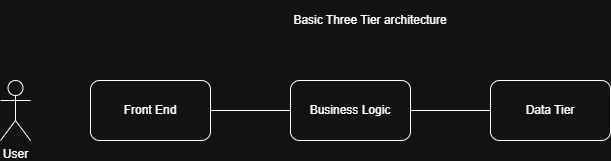
\includegraphics[width=0.8\textwidth]{basic-architecture} % Change to your filename
        \caption{Three tier architecture}
        \label{fig:drawio-diagram}
    \end{figure}


    \chapter{Architecture examples}


\end{document}
